\chapter{Die Arten} \label{ch:die_arten}

\tcbset{fonttitle=\bfseries\large,fontupper=\normalsize\sffamily,colback=myred,colframe=black,colbacktitle=mytopblue,coltitle=black,center title}

Obwohl die spielbaren Arten nur eine handvoll der vielen Lebensformen in den heimlichen Landen sind, sind gerade sie es die das meiste Gebiet ihr eigen nennen können. Sie sind es, die am innovativsten, überlegensten und kooperativsten sind. Auch wenn die Drachen mächtiger, die Vampiere schneller und die Dämonen geschickter sind, sind es nicht diese Arten die die großen Flächen des Kontinents besiedelten. In diesem Kapitel werden die spielbaren Arten vorgestellt, ihre Profilwerte präsentiert und ihre Fähigkeiten niedergelegt.

\section*{Die Genetik}
Die Genetik hängt von den Symbolen der Karten aus der Charaktererstellung ab. Jede der 7 Karten gewährt einen Rang in zur Symbol passenden Genetik.
Dabei ist ein maximaler Rang von 5 zu erreichen. Sollte jemand mehr als 5 Karten eines Symbols haben wird dies als Rang 5 gewertet und die übrigen verfallen. Man erhält auch alle Bonis der Ränge die man überschritten hat. \\
\textbf{Bsp.} \textit{Spieler 1 hat 2 Herz, 3 Pik und 3 Karo Karten bei seiner Charaktererstellung und Spieler 2 hat 1 Pik und 6 Kreuz. Spieler 1 hätte nun Rang 3 sowohl in der Pik, wie auch Karo Genetik, aber nur Rang 2 in der Herz Genetik. Spieler 2 hätte dagegen Rang 5 in der Kreuz Genetik, würde somit alle Kreuz Genetik Bonis erhalten und Rang 1 in der Pik Genetik.}

\section*{Rasse}
In \textit{Ludus Mortis} wird der Begriff der Rasse abweichend von der wissenschaftlich korrekten Weise verwendet. Er entspricht viel ehr einer Einteilung, welche die Draekolin verwenden, um besondere Merkmale an Kreaturen zu gewichten.

\subsection*{Kratzer}
Die klassischen Kreaturen der grünen Natur finden sich zusammen mit allerlei anderen Wesen unter der Kategorie der Kratzer. Diese Tiere leben in einem Umfeld an dass sie sich über Generationen angepasst haben und mit ihrer perfektionierten Lebensart meistern. Auch wenn einige Kratzer in der Lage wären Gegenstände zu verwenden wird der Großteil von ihnen ihre angeborenen Waffen über Objekte präferieren. Kratzer erhalten im \textbf{unbewaffneten Kampf} ein \textbf{Waffenbonus} von +1. Dieser Bonus erhöht sich mit dem Erreichen jeder vollen Zehnergefahrenstufe (Also 10 und 20) um eins.

\subsection*{Mechanismen} \label{mechanismus}
Mechanismen bestehen in der Regel aus Metall, Holz und anderen Baustoffen. Sie werden durch das Spiritfeld \textit{am Leben} gehalten und sind selten in der Lage emotionale Regungen zu spüren. Die mechanische Spielerart nennt sich \textit{\nameref{art:mrots}} und wurde von den Ghulen erbaut. Aufgrund ihrer Bestandteile sind Mechanismen in der Regel \textbf{nicht} in der Lage zu \textbf{ertrinken} oder Giftwunden zu sammeln. Jeder Effekt der ein Mechanismus \textbf{Giftwunden} hinzufügen würde fügt ihm im Zuge von Verätzungen \textbf{Wunden} zu. Da dieser Schaden jedoch eher geringer ausfallen wird, wird der Wert an Wunde \textbf{halbiert}. Würde einem Mechanismus eine Vergiftung zu geteilt werden, so erleidet er lediglich 5 Wunden. Eine weiter Auswirkung der mangelnden biologischen Bestandteile ist, dass der Mechanismus \textbf{nicht} durch Heileffekt, wie z.B. Heilkräuter o.Ä., \textbf{geheilt} werden kann. Die einzige Möglichkeit stellen \textit{Reperaturen} da, die teilweise durch den Mrot selber oder durch z.B. Orks oder ansässige Mechaniker durchgeführt werden können.

\subsection*{Mischlinge}
Die Draekolin warfen unter die Kategorie des Mischling all diese Kreaturen die in der Lage waren ihre Umwelt so stark anzupassen, dass sie diese gefügig machen lassen konnten. Neben dem Menschen sind z.B. die Ghule ein hervorragendes Beispiel für diese Kategorie. Beide Arten nutzen Werkzeuge, Ressourcen und andere Lebewesen aus um ihre Zivilisationen zu errichten und ihr Leben nach und nach zu verfeinern. Den Mischlingen fällt es viel einfacher sich zivilisiert zu verhalten, Gegenstände zu verwenden und zu erschaffen, so dass Spielleiter dazu angehalten sind, derartige Proben und Rollenspiele Mischlingskreaturen zu vereinfachen. Im Gegenzug hierzu sind sie allerdings draußen in der Wildnis schnell aufgeschmissen und verlieren leicht die Überhand wenn ihre wertvollen Entwicklungen nicht mehr funktionieren.

\subsection*{Spirit}
Kreaturen deren Existenz mit dem Wohlbehalten des Spiritfeldes zusammenhängt werden Spiritkreaturen genannt. Auch wenn die Draekolin sich selbst nicht als Teil dieser Kategorie ansehen, sind sie das Sinnbild dieser. Mit jedem sterbenden Engelsstein zerbröckelte ihre eigene Kraft bis, sie eines Tages zusammen mit dem letzten dieser Zugrunde gehen wird. Spiritkreaturen sind mächtige Manesfestatoren die in der Lage sind unglaubliche \textit{Wunder} zu verbringen.

% = = = = = = = = = = = = = = = = %
\clearpage
% = = = = = = = = = = = = = = = = %

\section{Draekolin} \label{art:draekolin}

		\begin{figure}[htbp]
		        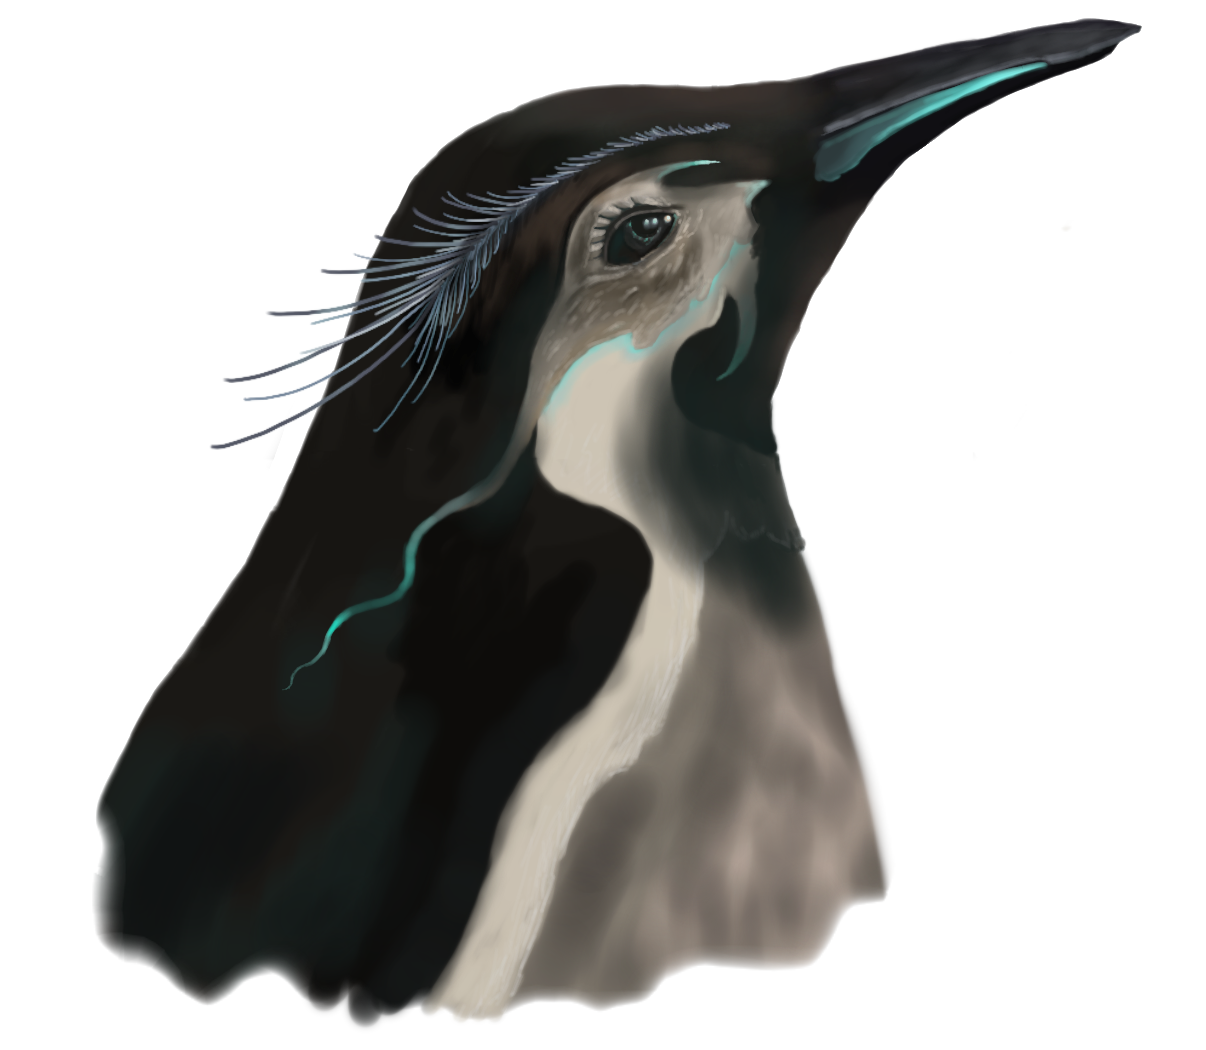
\includegraphics[width=8cm]{Pictures/Draekolin.png}
		        %\caption{Draekolin}
             \label{fig:Draekolin}
        \end{figure}
        
Sie werden die Boten des Frosts genannt, die Speere des Meeres, die Beschützer der Unruhe. Sie sind nicht bloß Krieger auf dem Land und Könige der Meere sondern auch mächtige Wachen des Wissens. Auch wenn ihre geringe Körpergröße und ihr langsame Geschwindigkeit auf dem Land ein großes Hindernis für die Frackträger darstellen, können sie die ihnen feindliche Umgebung anpassen und mit Hilfe von Manifestationen zu ihren Gunsten drehen. 
Die Draekolin leben in Ansammlung in der Nähe der lebenswichtigen Küsten. Ihre ranglose Gesellschaft verzichtet auf Kategorisierungen und sieht sich als überlegenende Schutzmacht ihrer Umgebung. Sie schützen aussterbende Rassen, jagen überbevölkernde und teilen ihren Rat mit niederen Zivilisationen. Als eine der wissenschaftlich führenden und spirituell mächtigsten Arten haben die verwandten der Pinguine eine große Anerkennung unter wissensgierigen Arten sicher.

\section*{Artenmerkmale}

\begin{tcolorbox}[title=Artenwerte,tabulars={@{\extracolsep{\fill}\hspace{5mm}}cccc@{\hspace{5mm}}},boxrule=0.5pt]
    \textbf{Wunden} & \textbf{Gift} & \textbf{Psyche} & \textbf{Bewegung} \\\hline
    40 & 10 & 15 & 5\\ \hlineB{3}
    \multicolumn{2}{ r| }{\textbf{Rasse:}} & \multicolumn{2}{ c }{Spirit} \\
    \multicolumn{2}{ r| }{\textbf{Größe:}} & \multicolumn{2}{ c }{Mittel, ca. 1.6 m} \\
    \multicolumn{2}{ r| }{\textbf{Gewicht:}} & \multicolumn{2}{ c }{ca. 30 kg} 
\end{tcolorbox}

\subsection*{Genetik der Draekolin}
\vspace*{0.75 cm}

\begin{tcolorbox}[title= Herz Genetik, colbacktitle=red, tabulars={@{\extracolsep{\fill}\hspace{5mm}}lc@{\hspace{1mm}}}, boxrule=0.5pt]
    \textbf{Rang 1:} & +2 auf Gewandtheit \\
    \textbf{Rang 2:} & Aktion \verweis{sk:eiskalter_hauch}\\
    \textbf{Rang 3:} & +2 auf Charisma\\
    \textbf{Rang 4:} & Aktion \verweis{sk:blendender_glanz}\\
    \textbf{Rang 5:} & +1 auf deine Bewegung\\
\end{tcolorbox}
\vspace*{0.4 cm}

\begin{tcolorbox}[title= Pik Genetik,colbacktitle=gray, tabulars={@{\extracolsep{\fill}\hspace{5mm}}lc@{\hspace{1mm}}}, boxrule=0.5pt]
    \textbf{Rang 1:} & +5 auf Wundenmaximum \\
    \textbf{Rang 2:} & +2 auf Robustheit \\
    \textbf{Rang 3:} & Aktion \verweis{sk:eismantel} \\
    \textbf{Rang 4:} & Aktion \verweis{sk:ruf_der_ahnen} \\
    \textbf{Rang 5:} & Passive \verweis{sk:eishart} \\
\end{tcolorbox}
\vspace*{0.4 cm}

\begin{tcolorbox}[title= Karo Genetik,colbacktitle=red, tabulars={@{\extracolsep{\fill}\hspace{5mm}}lc@{\hspace{1mm}}}, boxrule=0.5pt]
    \textbf{Rang 1:} & +2 auf Spirit \\
    \textbf{Rang 2:} & +2 im Element Frost \\
    \textbf{Rang 3:} & Aktion \verweis{sk:sternenstaub} \\
    \textbf{Rang 4:} & Passive \verweis{sk:kaelte} \\
    \textbf{Rang 5:} & +2 auf Intelligenz und +1 auf Spirit \\
\end{tcolorbox}
\vspace*{0.4 cm}

\begin{tcolorbox}[title= Kreuz Genetik,colbacktitle=gray, tabulars={@{\extracolsep{\fill}\hspace{5mm}}lc@{\hspace{1mm}}}, boxrule=0.5pt]
    \textbf{Rang 1:} & +1 auf Spirit \\
    \textbf{Rang 2:} & Aktion \verweis{sk:eiskalter_blick} \\
    \textbf{Rang 3:} & Aktion \verweis{sk:ins_exil} \\
    \textbf{Rang 4:} & +2 auf Geschicklichkeit \\
    \textbf{Rang 5:} & +2 Waffenbonus auf Speere \\
\end{tcolorbox}

\subsection*{Grundzüge}
Jeder Draekolin hat von Geburt an eine besonders Verbindung mit der Kälte, dies äußert sich auch in ihren Fähigkeiten. \\
Dein Charakter verfügt von Beginn an über die Aktionen: \verweis{sk:abkuehlen} und \verweis{sk:frostschlag}, sowie über die Passive: \verweis{sk:eisbrecher}.       

\subsection*{Abkühlen} \label{sk:abkuehlen}
Flackernd verstummen Fackeln, leise gefrieren Tümpfel und frostig kühl wird die Luft. Mit einem leisen Brausen durchfährt das sanfte Pusten der Kälte den geweihten Zirkel des Weiß. \\
\textbf{Grundwert:} Spirit \\
\textbf{Kenntnisschwelle:} 3 \\
\textbf{Maximale Kenntnis:} 5 \\
\textbf{Anforderung:} Stationär 15+ \\
\textbf{Effekt:} Beende alle \textit{\nameref{ef:brennend} Effekte} im Radius \textbf{FK*2} Meter. Jede Kreatur mit dem Leiden \textit{\nameref{ef:gefroren}} im Reichweite erleitet \textit{\nameref{ef:element} Frost} Wunden. \textbf{Bonus:} \textit{\nameref{ef:element} Frost}

\subsection*{Eisbrecher} \label{sk:eisbrecher}
Die gefrorenen Muskulaturen zerschellen unter den kalten Krallen des wohlhabenden Zorns der Draekolinangriffe. Kein Blut wird fließen keine Körper mehr pulsieren. \\
\textbf{Effekt:} \textit{Passiv.} Alle deine \textit{Angriffe} gegen Kreaturen mit dem Leiden \textit{\nameref{ef:gefroren}} verursachen \textit{\nameref{ef:element} Frost} mehr Schaden.

\subsection*{Frostschlag} \label{sk:frostschlag}
Mit einem flinken Schlag zerpeitscht eine Eiskette aus feinsten Strukturen die oberen Hautschichten des überraschten Opfers. Der schmerzerfüllte Aufschrei des gepeinigte Opfers surrt durch die kalte Luft, bis ein erneuter Aufprall der blutgetränkte Peitsche wieder niederschlägt.\\
\textbf{Grundwert:} Spirit\\
\textbf{Kenntnisschwelle:} 10 \\
\textbf{Anforderung:} $\Karo{}$ \\
\textbf{Reichweite:} 0.5 m \\
\textbf{Effekt:} \textit{Angriff (Physisch))[X]}. Falls das Ziel vor dem Angriff \textit{\nameref{ef:gefroren}} war, bleibt es dies auch. \textbf{Bonus:} \textit{Element Frost}.

\begin{table}[h!]
    \centering
    \begin{tabular}{|>{\columncolor[RGB]{247, 216, 212}}l|}
    \btrule{1pt}
    \arrayrulecolor{black}
    \\
    \textbf{\large Draekolin}\\
    \\
        \begin{tabular}{c|c|c}
           \rowcolor{myred} \begin{tabular}{c}
               \rowcolor{myred}\textbf{Gefahren-}  \\
                \rowcolor{myred} \textbf{wert}\\ 
            \end{tabular} & \textbf{Fähingkeiten} & \textbf{Ausprägung}\\
            \hline
            \rowcolor{myred} 1. & -- & Pfad \\
            \rowcolor{myblue} 2. & 1x Simpel & Eisig \& Pfad \\
            \rowcolor{myred} 3. & 1x Erweitert & Pfad\\
            \rowcolor{myblue} 4. & 1x Komplex &  Charakterentw. \\
            \rowcolor{myred} 5. & -- &  Pfad\\
            \rowcolor{myblue} 6. & -- & Körperentw. \\
            \rowcolor{myred} 7. & 2x Simpel &  Pfad \\
            \rowcolor{myblue} 8. & 1x Erweitert & --\\
            \rowcolor{myred} 9. & 1x Komplex & Pfad\\
            \rowcolor{myblue} 10. & -- & Fährtenleser \\
            \rowcolor{myred} 11. & -- & Charakterentw.\\
            \rowcolor{myblue} 12. & 1x Simpel & Pfad\\
            \rowcolor{myred} 13. & 2x Erweitert & Charakterentw.\\
            \rowcolor{myblue} 14. & 1x Komplex & --\\
            \rowcolor{myred} 15. & -- & Pfad\\
            \rowcolor{myblue} 16. & -- & Körperentw.\\
            \rowcolor{myred} 17. & 1x Simpel & Charakterentw.\\
            \rowcolor{myblue} 18. & 1x Erweitert & Pfad \\
            \rowcolor{myred} 19. & 2x Komplex & --\\
            \rowcolor{myblue} 20. & -- & Körperentw.\\
            \rowcolor{myred} 21. & -- & Charakterentw.\\
            \rowcolor{myblue} 22. & 2x Simpel & Pfad\\
            \rowcolor{myred} 23. & 2x Erweitert & Charakterentw.\\
            \rowcolor{myblue} 24. & 2x Komplex & Körperentw.\\
            \rowcolor{myred} 25. & Wächter des Eises & -- \\
            %\rowcolor{myblue} 26. & -- & Pfad\\
            %\rowcolor{myred} 27. & 2x Simpel & \\
            %\rowcolor{myblue} 28. & 2x Erweitert& \\
            %\rowcolor{myred} 29. & 2x Komplex & \\
            %\rowcolor{myblue} 30. &  (Spezifisch) & Pfad\\
        \end{tabular}\\
        \rowcolor{myred}\\
        \btrule{1pt}
    \end{tabular}
\end{table}

\section*{Die Pfade der Kälte}
Der Draekolinspieler wandert auf einem der vier Pfaden der Kälte. Dem mysteriösen und unergründlichen Pfad des Nebels, dem harten und besonders kühlen Pfad des Eises, dem traditionellen und spirituell geprägten Pfad des Frostes oder doch auf dem erkundenden Pfad des Schnees.


\subsection*{Pfad des Nebels $\Herz{}$}
Mit dem Pfad des Nebels beschreitest du die geheimnisvollsten Wege der Lehre der Draekolin. Nicht jeder ist dieser Herausforderungen gewachsen und kehrt aus dem Nebel zurück. \\
\textbf{Boni:} +1 \textit{\nameref{ef:element} Frost}. \\
\textbf{Anfangsausrüstung:} \textit{Umhängetasche} mit deinen \textit{persönlichen Gegenständen}, einem \textit{\nameref{ar:bundderschritte}} und einer \textit{einfachen Waffe}.\\
\textbf{Startfähigkeit:} \verweis{sk:schleier_des_nebels}. \\

\subsubsection*{\fbox{1} Schleier des Nebels} \label{sk:schleier_des_nebels}
Nach der Wahl dieses Pfades bist du in der Lage dein Auftreten gegenüber anderen zu verschleiern. Dich umgibt eine mysteriöse Präsenz die du dir in Interaktionen mit anderen Kreaturen zunutze machen kannst.\\
\textbf{Effek:} +2 auf Überzeugungs-, Charm- und Täuschungsproben. \\
\textbf{Steigerung [15]:} Überzeugungs- und Charmproben werden um ein Grad erleichtert.\\
\textbf{Steigerung [25]:} Täuschungsproben gelten solange sie nicht unmöglich sind als erfolgreich.\\

\subsubsection*{\fbox{2} Nebelschritt} \label{sk:nebelschritt}
Mit dem erreichen des Gefahrenwerts 2 erhältst du die Aktion Nebelschritt.\\
\\
Auf den schweren Wegen durch das Land ist es nicht selten nützlich, sich den Augen der anderen Völker zu entziehen zu können.\\
\textbf{Grundwert:} Spirit \\
\textbf{Kenntnisschwelle:} 10 \\
\textbf{Anforderung:} $\Herz{}$ 22+ \\
\textbf{Effekt:} Bewege dich bis zu deiner Bewegungsreichweite. Du kannst bis zu deiner nächsten Aktion nicht als Ziel gewählt werden. Setze deinen \textbf{Status} auf \textbf{Bewegend}.

\subsubsection*{\fbox{3} Tänzelnde Schritte} \label{sk:tänzelnde_schritte}
Ab Gefahrenwert 3 erhältst du Zugang zu der Passiven Tänzelnde Schritte.\\
\\
Mit einer eisernen Präzision nimmt der Draekolin seine Umgebung war. Er weiß welcher Stein unruhig liegt und welcher Ast brechen wird. Er kann ohne Probleme mit seinem Schlag sich bewegen und sauber landen.\\
\textbf{Effekt:} \textit{Passiv.} Nach einer Angriffsaktion kannst du dich um die Hälfte deiner Bewegung zusätzlich bewegen. Falls du dich bewegst setze deinen \textbf{Status} auf \textbf{Bewegend}.\\
\textbf{Steigerung [20]}: Die Weite deiner zusätzlichen Bewegung erhöht auch deine Bewegungsreichweite.

\subsubsection*{\fbox{5} Nebelschlag} \label{sk:nebelschlag}
Mit dem Erreichen des Gefahrenwertes 5 erhältst du die Aktion Nebelschlag.\\
\\
Das Skrivapack des Ostens nennt es den Tanzschlag oder Watschelklatsche. Diese niederlassende Worte werden der Wahrheit nicht einmal ansatzweise gerecht. Die präzisen Nebelschläge sind kunstvolle Angriff die ihre Opfer überraschen und in Sekunden schnelle besiegen können.\\
\textbf{Grundwert:} Geschicklichkeit \\
\textbf{Kenntnisschwelle:} 2 \\
\textbf{Anforderung:} 20+ \\
\textbf{Effekt:} \textit{Angriff (Physisch)}. Wurdest du seit deiner letzten Aktionsphase nicht angegriffen, dann werden die zugefügten Wunden dieses Angriffes verdoppelt. War deine letzte Aktion \verweis{sk:in_den_nebel} werden die Wunden verdreifacht.

\subsubsection*{\fbox{7} Nebelkreatur} \label{sk:nebelkreatur}
Ab Gefahrenwert 7 erhältst du die Passive Nebelkreatur.\\
\\
Ein Meister des Nebels kann selber entscheiden wann er gesehen werden möchte und wann er die Aufmerksamkeit lieber meiden möchten. Doch sollte der Zeitpunkt gekommen sein, so seien seine Gegner gewarnt, denn er tritt nicht leichtfüßig aus den Schatten.\\
\textbf{Effekt:} \textit{Passiv.} Solange du in den Kampf noch keine Wunden erlitten oder Angriff ausgeführt hast kannst du nicht als Ziel von Angriffen gewählt werden.\\
\textbf{Steigerung [23]:} Der Effekt gilt für jede Kampfrunde.

\subsubsection*{\fbox{9} In den Nebel} \label{sk:in_den_nebel}
Mit dem Erreichen des Gefahrenwertes 9 erhältst du Zugang zu der Macht der Aktion In den Nebel.\\
\\
Der Nebel birgt ein gutes Versteck, in das du dich zu Not mit deinen Verbündeten zurückziehen kannst.  \\
\textbf{Grundwert:} Gewandtheit \\
\textbf{Kenntnisschwelle:} 2 \\
\textbf{Reichweite:} 10 m
\textbf{Anforderung:} $\Kreuz{}$ 20+ \\
\textbf{Effekt:} Du und eine andere befreundete Kreatur in Reichweite können bis zu der jeweils nächsten Aktionsphase nicht als Ziel gewählt werden, außer sie haben erneut Wunden erlitten.\\
\textbf{Steigerung [15]:} Wähle bis zu zwei andere befreundete Kreaturen.\\
\textbf{Steigerung [25]:} Wähle eine befreundete Kreatur, alle anderen befreundeten Kreaturen in Reichweite können nicht als Ziel gewählt werden.

\subsubsection*{\fbox{12} Flüchtige Gestalt} \label{sk:verschwindende_gestalt}
Ab Gefahrenwert 12 erhältst du die Passive Flüchtige Gestalt.\\
\\
Das Wabern des Nebels kann ein mächtiges Schild in den Händen des rechten Nutzers sein. Ohne große körperliche Mühen ist es dem Draekolin möglich seinen Gegner aus zu manövrieren.  \\
\textbf{Effekt:} \textit{Passiv.} Wenn du Wunden erleidest, kannst du ein Zeichen für die oberste Karte deines Decks ansagen. Lege die oberste Karte ab. Falls das Zeichen übereinstimmt erleidest du nur die Hälfte der Wunden.\\

\subsubsection*{\fbox{15} Nebelschauder} \label{sk:nebelschaueder}
Mit dem erreichen des Gefahrenwertes 15 erhältst du die Aktion Nebelschauder.\\
\\
Manchen Kreaturen schaudert der Anblick des Nebels, dies auch nicht zu unrecht. Den die Krieger des Nebels machen ihn sich zu nutze um ihre Feinden psychischen Schaden zuzufügen.\\
\textbf{Grundwert:} Charisma \\
\textbf{Kenntnisschwelle:} 2 \\
\textbf{Anforderung:} 20+ \\
\textbf{Effekt:} \textit{Angriff (Psyche)}. Wurdest du seit deiner letzten Aktionsphase nicht angegriffen, dann werden die zugefügten Psychewunden dieses Angriffes verdoppelt. War deine letzte Aktion \verweis{sk:in_den_nebel} und gelingt diese Aktion, dann wird automatisch eine geistige Umnachtung beim Ziel erzeugt.

\subsubsection*{\fbox{18} Klang des Meeres} \label{sk:klang_des_meeres}
Mit dem erreichen des Gefahrenwertes 18 erhältst du die Aktion Klang des Meere.\\
\\
Die unnatürlich reine, harmonische Stimme der feuchten Luft schwingt in einem Rhythmus der Eleganz und Fremdnis. Er lockt die Neugierigen und Gierigen genau da hin wo ihr Ende auf sie wartet.\\
\textbf{Grundwert:} Intelligenz \\
\textbf{Kenntnisschwelle:} 2 \\
\textbf{Anforderung:} 20+ \\
\textbf{Effekt:} Senke den Schaden aller ausgeführten Aktionen im Radius von 5 m bis zu deiner nächste Aktion um \textbf{FK}.


\subsubsection*{\fbox{22} Ritter des Nebels} \label{sk:ritter_des_nebels}
Ab Gefahrenwert 22 erhältst du die Passive Ritter des Nebels.\\
\\
Die Bezeichnung Ritter des Nebels gaben die Norks den Hohepriestern des frierenden Nebels. Sie, die niemand finden wird der sie zynisch sucht, sind die erfahrensten Schatten im Ungewissen. Sie sind die Bringer der Botschaft. Sie sind die Ankömmlinge am Ende des Pfades.\\
\textbf{Effekt:} Du ziehst einen Schleier aus Nebel hinter dir her. Dieser Dunst verbessert dein Ausweichen im Kampf um +6. Außerdem kannst du jederzeit ein Reittier des Nebels rufen, welches dir sofort erscheint.   


\subsection*{Pfad des Eises $\Pik{}$} 
Um die Klarheit des Eises zu erlangen muss der Draekolin sich auf die Lehre des logischen Wissens begeben. Er befreit sein Denken von emotionalen Missleitungen und öffnet sich der striken, optimalen Vorgehensweise. \\
\textbf{Boni:} +2 \textit{\nameref{ef:element} Frost}. \\
\textbf{Anfangsausrüstung:} \textit{Umhängetasche} mit deinen \textit{persönlichen Gegenständen}, einem \textit{\nameref{ar:feldflaschetrinkschlauch}} und einer \textit{einfachen Waffe}.\\
\textbf{Startfähigkeit:} \verweis{sk:eisiges_blut}\\

\subsubsection*{\fbox{1} Eisiges Blut} \label{sk:eisiges_blut}
Dein Blut ist viel Kälter als das der anderen Arten, was dir auch bei wärmeren Temperaturen einen regenerativen Vorteil verschafft.\\
\textbf{Effekt:} Heile am Anfang einer Kampfrunde bis zu 2 deiner Wunden. Außerhalb des Kampfes regenerierst du 2-fach so viele Wunden\\
\textbf{Steigerung [15]:} Regeneration erhöht sich auf 5 Wunden (bzw. 5-fach Regeneration) \\
\textbf{Steigerung [25]:} Regeneration erhöht sich auf 10 Wunden (bzw. 10-fach Regeneration).

\subsubsection*{\fbox{2} Frostpanzer} \label{sk:frostpanzer}
Mit dem Erreichen des Gefahrenwertes 2 erhältst du die Aktion Frostpanzer.\\
\\
Ein krustige Schicht an eisigen Strukturen spinnt sich über den Körper des verharrenden Draekolins und bildet eine stabile glitzernde Rüstung.\\
\textbf{Grundwert:} Spirit \\
\textbf{Kenntnisschwelle:} 10 \\
\textbf{Anforderung:} Stationär 20+ \\
\textbf{Effekt:} Bis zu deiner nächsten Aktionsphase steigt deine Robustheit um 2 + \textbf{FK} und kannst wählen ob du ein 5 + \textbf{FK} großen Schild bekommst und dafür das Leiden \verweis{ef:gefroren} erhältst.

\subsubsection*{\fbox{3} Eisige Bedrohung} \label{sk:eisige_bedrohung}
Ab Gefahrenwert 3 erhältst du die Passive Eisige Bedrohung.\\
\\
Deine pure Präsenz im spiritnahen Feld deiner Feinde schlägt sich vehement auf sie nieder. Ihr Atem wird schwerer und ihrer Körper beginnt zu zittern.\\
\textbf{Effekt:} \textit{Passiv.} Für Bewegung von Feinden mit dem Leiden \verweis{ef:gefroren} im 5 m Radius zählen jeder Meter wie zwei.\\
\textbf{Steigerung [15]:} Der Radius ist nun 10 m.

\subsubsection*{\fbox{5} Frostwall} \label{sk:frostwall}
Gefahrenwert 5 gewährt dir die Aktion Frostwall.\\
\\
Wie die Umrisse der Sonnen kristallisieren sich die feinen Eisstrukturen um den stolzen Frackträger. Versuche von törichten Angreifern den Forstschutz zu durchdringen werden mit scharfen Eissplittern empfangen. \\
\textbf{Grundwert:} Spirit\\
\textbf{Kenntnisschwelle:} 10 \\
\textbf{Anforderung:} $\Karo{}$ 18+ \\
\textbf{Effekt:} Kreiere bis zu deiner 1 + FK Aktionsphase ein Frostschild um dich. Für die Dauer des Frostschildes kannst du selber keine Nahkampfangriffe ansagen und keine normalen Reaktionsangriffe ausführen. Wann immer eine Kreatur dich im Nahkampf angreift führst du einen Nahkampfangriff mit der obersten Deckkarte gegen sie aus bevor sie ihren Angriff durchführt. Du kannst das Frostschild als kostenfrei Bonusaktion abbrechen.

\subsubsection*{\fbox{7} Wohltuende Kälte} \label{sk:wohltuende_kaelte}
Durch das Erreichen des 7ten Gefahrenwertes wird die Passive Wohltuende Kalte dein Eigen.\\
\\
Die Anwesenheit von Kälte tut dir gut. Es durch fährt deine Venen und gibt dir ein angenehmes Gefühl von Heimat.\\
\textbf{Effekt:} \textit{Passiv.} Für jede gegnerische Kreatur mit dem Leiden \verweis{ef:gefroren} in unmittelbarer Nähe (10 m) erhältst du einen Grad an Besserung.

\subsubsection*{\fbox{9} Befreiung} \label{sk:befreiung}
Mit dem Erreichen des Gefahrenwertes 9 erhältst du die Aktion Frostpanzer.\\
\\
Die glänzenden Strukturen um den Draekolin schießen schlagartig von ihm weg und durchschlagen mit Leichtigkeit ihre Umgebung. Wie feine Dartpfeils flattern sie durch die Luft bis sie in ihr Ziel einschlagen. \\
\textbf{Grundwert:} Spirit \\
\textbf{Kenntnisschwelle:} 10 \\
\textbf{Anforderung:} aktiver \textit{\nameref{sk:frostwall}}\\
\textbf{Effekt:} \textit{Angriff (Physisch)}. \textit{Alle} Kreaturen innerhalb von 4 + FK m werden von dem Angriff getroffen und verteidigen gegen diesen. Alle Kreaturen die Wunden erleiden erleiden \verweis{ef:gefroren}. Dein \textit{\nameref{sk:frostwall}} gilt als beendet.\\
\textbf{Steigerung [20]:} \verweis{sk:frostwall} beilbt erhalten.

\subsubsection*{\fbox{12} Frostbote} \label{sk:forstbote}
Durch das Erreichen des 12ten Gefahrenwertes wird die Passive Frostbote dein eigen.\\
\\
War der Frost eins der Feind der Draekolin, so haben die Gelehrten des Eises daraus ihre größte stärke gemacht. \\
\textbf{Effekt:} \textit{Passiv.} Du kannst Karten deines Gegenzeichens gegen \verweis{ef:gefroren} Kreaturen wie Karten deines eigenen Zeichens behandeln.

\subsubsection*{\fbox{15} Die Klarheit des Eises} \label{sk:dieklarheitdeseises}
Gefahrenwert 15 gewährt dir die Aktion Die Klarheit des Eises.\\
\\
Die Mythen besagen, dass die Draekolin durch das Eis klar, also in die Zukunft, sehen könnten. So sagt man sich zumindest. Überraschend wie nah das Gemunkel an die Wahrheit heranrückt. \\
\textbf{Grundwert:} Spirit \\
\textbf{Kenntnisschwelle:} 5 \\
\textbf{Anforderung:} $\Herz{}$ 18+ \\
\textbf{Effekt:} Wähle eine Menge an Kartenstapeln aus, die deiner Fähigkeitskenntnis plus eins entsprechen. Decke jeweils die oberste Karte auf dem Stapel auf, so dass du und deine Mitspieler wissen welche die nächste Karte sein wird, die gezogen/aufgedeckt wird. Lassen sie offen liegen bis sie gezogen/abgelegt wird.

\subsubsection*{\fbox{18} Klirrende Kälte} \label{sk:klirrende_kälte}
Gefahrenwert 18 gewährt dir die Passive Klirrende Kälte.\\
\\
Deine Kälte lässt selbst die Tapfersten Krieger bis in ihr Mark erzittern.\\
\textbf{Effekt:} \textit{Passiv.} Falls du oder dein Angreifer das Leiden \verweis{ef:gefroren} haben, erleidest du bei dem Angriff \textbf{FK} + 3 weniger Schaden.

\subsubsection*{\fbox{22} Frostfürst} \label{sk:Frostfürst}
Gefahrenwert 22 gewährt dir die Passive Frostfluch.\\
\\
Du ziehst die Kälte quasi \textit{magisch} an. Selbst die Kreaturen, die schmerzhaft deiner Kälte ausgesetzt sind,  können deinem Ruf nicht widerstehen.\\
\textbf{Effekt:} \textit{Passiv.} Gegnerische Kreaturen in Nahkampfreichweite zu dir mit dem Leiden \verweis{ef:gefroren} müssen dich als Ziel ihrer Aktion wählen.




\subsection*{Pfad des Frost $\Karo{}$}
Die Schritte auf dem Pfad des Frosts sind geprägt von Planung und Taktiken. Um Erfolge zu feiern müssen Strategien aufgehen und Schritte im Vorhinein durchdacht werden. \\
\textbf{Boni:} +3 \textit{\nameref{ef:element} Frost}. \\
\textbf{Anfangsausrüstung:} \textit{Umhängetasche} mit deinen \textit{persönlichen Gegenständen} und einem \textit{\nameref{ar:bundderschritte}}.\\
\textbf{Startfähigkeit:} \verweis{sk:frostmantel}\\

\subsubsection*{\fbox{1} Frostmantel} \label{sk:frostmantel}
Die Umarmung des Frostes ist ein wunderbares Geschenk das einen unglaublichen Wert mit sich bringt. Ganze Heerscharen an Feinde werden auf einmal zu nutzlose Widersacher.\\
\textbf{Effekt:} Du bist immun gegenüber \verweis{ef:gefroren} und kannst nicht als Ziel von Aktionen des Elements Frost gewählt werden.

\subsubsection*{\fbox{2} Frostwinde} \label{sk:frostwinde}
Gefahrenwert 2 gewährt dir die Aktion Frostwinde.\\
\\
Mit dem Frost geht auch das Wetter einher. So war eine der ersten Errungenschaften der Draekolin die Wettermanipulation in Form von unkontrollierten frostigen Winden. \\
\textbf{Grundwert:} Spirit \\
\textbf{Kenntnisschwelle:} 2 \\
\textbf{Anforderung:} 18+ \\
\textbf{Effekt:} Belege alle Kreaturen in einem Radius von 10 m um dich mit dem Leiden \verweis{ef:gefroren}.

\subsubsection*{\fbox{3} Geburt des Frost} \label{sk:geburt_des_frost}
Gefahrenwert 3 gewährt dir die Passive Geburt des Frost.\\
\\
Mit der Geburt im stärksten Frost des Landes geht eine starke Verbindung einher, die sich nach und nach zeigt.\\
\textbf{Effekt:} \textit{Passiv}. +2 \textit{\nameref{ef:element} Frost}.\\
\textbf{Steigerung [15]:} Weitere +3 \textit{\nameref{ef:element} Frost}.\\
\textbf{Steigerung [25]:} Weitere +5 \textit{\nameref{ef:element} Frost}.

\subsubsection*{\fbox{5} Eissturm} \label{sk:eissturm}
Gefahrenwert 5 gewährt dir die Aktion Eissturm.\\
\\
Einigen Draekolin haben die Frostwinde nicht genügt. Sie begaben sich auf die zerstörerischen Wege der Eisstürme. Die Einforderung dieser kostete viele Opfer, doch sind sie als Schutz vor Eindringlingen aus der heutigen Gesellschaft der Draekolin nicht mehr wegzudenken. \\
\textbf{Grundwert:} Spirit \\
\textbf{Kenntnisschwelle:} 2 \\
\textbf{Anforderung:} $\Karo{}$ 18+ \\
\textbf{Effekt:} Lege eine Karte ab. \textit{Angriff (Physisch)}, trifft alle anderen Kreaturen im 5 m Radius um dich herum. Alle durch diese Aktion verwundeten Kreaturen erleiden das Leiden \verweis{ef:gefroren}.
\textbf{Bonus:} \textit{\nameref{ef:element} Frost}.\\
\textbf{Steigerung [15]:} Der Radius ist nun 10 m.\\
\textbf{Steigerung [20]:} Der Radius ist nun 15 m.

\subsubsection*{\fbox{7} Permafrost} \label{sk:permafrost}
Gefahrenwert 7 gewährt dir die Passive Permafrost.\\
\\
Die Schneide des Frostes fährt sachte durch die Geläuterten ohne ihrer Reinheit Schaden zu zufügen. So werden auch die erfahrenen Diener des Forstes wissen die, die sie befreit haben in den Kunst der erfrischenden Wahrheit zu belassen. \\
\textbf{Effekt:} \textit{Passiv}. Alle deine Angriffe entfernen das Leiden \verweis{ef:gefroren} nicht.


\subsubsection*{\fbox{9} Wärmender Frost} \label{sk:waermender_frost}
Gefahrenwert 9 gewährt dir die Aktion Wärmender Frost.\\
\\
Wie Worte die mit Geschichten vergangener Zeiten deine Seelen erhellen, kann auch der Frost dem Körper von Individuen Wärme und Geborgenheit spenden. Das ungewohnte Frieren driftet dann langsam ab in ein wohl wollendes inneres Glühen. \\
\textbf{Grundwert:} Spirit \\
\textbf{Kenntnisschwelle:} 2 \\
\textbf{Anforderung:} Stationär 25+ \\
\textbf{Effekt:} Wähle eine Kreatur, diese Kreatur verliert das Leiden \verweis{ef:gefroren} und erhält die Begünstigung \verweis{ef:besserung} mit dem gleichen Grad.

\subsubsection*{\fbox{12} Absoluter Nullpunkt} \label{sk:absoluter_nullpunkt}
Gefahrenwert 12 gewährt dir die Passive Absoluter Nullpunkt.\\
\\
Auch wenn der Frost nicht im wahren Sinne endlich oder gar messbar wäre, so sind die Thermometer der Menschen begrenzt. Auch wenn das Erreichen dieses untersten Punktes für die Menschheit auf ewig verwert sein wird, so werden die Krieger des Frostes mit ein wenig Hoffnung diesen über ihre Umgebung bringen können. \\
\textbf{Effekt:} \textit{Passiv}. Wenn du jemanden mit dem Leiden \verweis{ef:gefroren} belegst, kannst du einmal pro Kampfrunde den folgenden Zusatzeffekt zum Leiden hinzufügen: Du kannst dich die nächste Aktionsphase nicht Bewegen und nicht angreifen.\\
\textbf{Steigerung [20]:} Nun kann der Effekt zweimal pro Kampfrunde genutzt werden.

\subsubsection*{\fbox{15} Zerbrechen} \label{sk:zerbrechen}
Gefahrenwert 15 gewährt dir die Aktion Zerbrechen.\\
\\
Die Kälte des Frosts durchdringt den Körper. Er bindet die Organe und verfestigt ihn. Ein einziger Weiterer Schlag könnte diesen Körper brechen und zerreißen. \\
\textbf{Grundwert:} Spirit \\
\textbf{Kenntnisschwelle:} 2 \\
\textbf{Anforderung:} $\Karo{}$ 25+ \\
\textbf{Effekt:} \textit{Angriff (Physisch)}. Wenn eine Kreatur, die das Leiden \verweis{ef:gefroren} von dir erhalten hat, als Ziel eines Angriffes gewählt wird, wird der Effekt von \verweis{ef:gefroren} verdoppelt. \textbf{Bonus:} \textit{\nameref{ef:element} Frost}.\\
\textbf{Steigerung [18]:} Der \verweis{ef:gefroren} Effekt wird verdreifacht.\\
\textbf{Steigerung [25]:} Der \verweis{ef:gefroren} Effekt wird vervierfacht.\\

\subsubsection*{\fbox{18} Frostgefängnis} \label{sk:frostphantom}
Gefahrenwert 18 gewährt dir die Passive Frostphantom.\\
\\
Wenn der Frost sich in deinen Gliedern einmal fest gesetzt hat wird es ein schwieriger Akt ihm wieder zu entkommen. Die verringerte Präzision macht es einem Kämpfer der dies bereits gesehen hat leichter, deinen Angriffen auszuweichen. \\
\textbf{Effekt:} \textit{Passiv}. Deine \textit{Blocken}- oder \textit{Ausweichen}- Aktionen gegen ein Angriff einer Kreatur mit dem Leiden \verweis{ef:gefroren} werden um den Grad des Leidens verbessert.

\subsubsection*{\fbox{22} Wille des Frost} \label{sk:wille_des_frost}
Gefahrenwert 22 gewährt dir die Passive Wille des Frost.\\
\\
Die Präsenz deiner Frostgestallt ist all durchdringend. Mit einem leichten Signal schon kannst du die Kräfte des Spiritfeldes fassen und um ein Gegner binden als wäre es bloß ein Spiel. \\
\textbf{Effekt:} \textit{Passiv}. Belege zu beginn deiner Aktionsphase eine Kreatur in 15 m mit dem Leiden \verweis{ef:gefroren}.



\subsection*{Pfad des Schnee $\Kreuz{}$}
....................\\
\textbf{Boni:} +2 \textit{\nameref{ef:element} Frost}. \\
\textbf{Anfangsausrüstung:} \textit{Umhängetasche} mit deinen \textit{persönlichen Gegenständen} und einer \textit{fortgeschrittenen Waffe}.\\
\textbf{Startfähigkeit:} \verweis{sk:bund_des_schnees} \\

\subsubsection*{\fbox{1} Bund des Schnees} \label{sk:bund_des_schnees}
\textbf{Effekt:} Du wählst bei der Wahl des Pfad einen Charakter als Gefährten. Wenn du oder dein Gefährte geheilt wird kannst du die Heilung halbieren um den anderen um die Hälfte des Wertes heilen.\\
\textbf{Steigerung [15]:} Du kannst die Hälfte der Wunden die dein Gefährte erleiden würde anstelle von ihm erleiden.



\subsubsection*{\fbox{2} Schneefall} \label{sk:schneefall}
Ab Gefahrenwert 2 erhältst du die Aktion Schneefall.\\
\\
Das feine Rieseln des fallenden Schnees wirbelt eine lockere Freude in das Herz der Vertreter der Kälte. Es ist wie eine Hoffnung in den Zeiten der Verzweiflung.\\
\textbf{Grundwert:} Spirit \\
\textbf{Kenntnisschwelle:} 3 \\
\textbf{Anforderung:} Stationär $\Kreuz{}$ \\
\textbf{Effekt:} Du und dein Gefährte erhalten Besserung in Höhe deines \textit{\nameref{ef:element} Frost} \\
\textbf{Steigerung [15]:} Alle anderen befreundeten Kreaturen erhalten die Hälfte an Besserung.

\subsubsection*{\fbox{3} Eisarsenal} \label{sk:eisarsenal}
Ab Gefahrenwert 3 erhältst du die Passive Eisarsenal.\\
\\
Der Frost, der von dir ausgeht, ist so kalt, dass es bei jeden, den du berührt, ein schmerzliches Brennen zurück lässt.\\
\textbf{Effekt:} \textit{Passiv.} Du kannst Axte, Schwerter, Speere aus Eis auf magische Weise erschaffen. Diese Waffe hat die normale Reichweite, aber als Bonus dein Element Frost. Es ist jedoch nur möglich eine dieser Waffen zeitgleich zu haben, so eine neue Waffe kreiert werden brauchst du dazu eine Aktion.\\
\textbf{Steigerung [15]:} Du kannst bis zu drei Waffen zeitgleich besitzen.

\subsubsection*{\fbox{5} Schneeball} \label{sk:schneeball}
Ab Gefahrenwert 5 erhältst du die Aktion Schneeball.\\
\\
Du erzeugst einen Schneeball, den du wie einen Wuftspeere auf dein Ziel wirfst.\\
\textbf{Grundwert:} Geschicklichkeit \\
\textbf{Kenntnisschwelle:} 2 \\
\textbf{Anforderung:} $\Kreuz{}$ \\
\textbf{Reichweite:} Kraft/2 in m \\
\textbf{Effekt:} \textit{Angriff (Physisch)}. Der Schneeball wird wie eine Waffe des \verweis{sk:eisarsenal} behandelt.

\subsubsection*{\fbox{7} Frostigewaffen} \label{sk:frostigewaffen}
Ab Gefahrenwert 7 erhältst du die Passive Frostigewaffen.\\
\\
Der Frost, der von dir ausgeht, ist so kalt, dass es bei jeden, den du berührt, ein schmerzliches Brennen zurück lässt.\\
\textbf{Effekt:} \textit{Passiv.} Du kannst deine Waffe mit einer Schicht Eis überziehen, sodass diese bei einem erfolgreichen Angriff dem Ziel das Leiden \verweis{ef:gefroren} Zufügt in Höhe des halben wertes von deinem \textit{\nameref{ef:element} Frost}. Waffen des Eisarsenals sind direkt von dem Effekt betroffen und fügen \verweis{ef:gefroren} in Höhe deines \textit{\nameref{ef:element} Frost} zu (additiv mit der Passiven \verweis{sk:kaelte}).

\subsubsection*{\fbox{9} Unterkühlen} \label{sk:unterkühlen}
Ab Gefahrenwert 9 erhältst du die Aktion Unterkühlen.\\
\\
Leichter Schnee fällt in dem Zielbereich und unterkühlt alle Kreaturen in dem Bereich.\\
\textbf{Grundwert:} Spirit \\
\textbf{Kenntnisschwelle:} 2 \\
\textbf{Anforderung:} $\Kreuz{}$ \\
\textbf{Reichweite:} 20 m \\
\textbf{Effekt:} Jede Kreatur im Zielbereich erleidet das Leiden \verweis{ef:gefroren}, die Höhe der Grades entspricht der obersten Karte.

\subsubsection*{\fbox{12} Schockfrost} \label{sk:schockfrost}
Ab Gefahrenwert 12 erhältst du die Passive Schockfrost.\\
\\
Deine Waffen haben unter deiner Kälte eine schockierende Persönlichkeit entwickelt\\
\textbf{Effekt:} \textit{Passiv.} Anstelle dass das Leiden \verweis{ef:gefroren} Wunden verursacht bei einem deiner Angriffe mit einer Frostigenwaffe, kannst du dich entscheiden ob die Kreatur stattdessen die geistige Umnachtung \textit{Unter Schock} erhält.

\subsubsection*{\fbox{15} Neuschnee} \label{sk:neuschnee}
Ab Gefahrenwert 15 erhältst du die Aktion Neuschnee.\\
\\
Schnee stellt für dich kein Hindernis da, vielmehr hilft er dir dich zu konzentrieren besonders wenn er frisch gefallen ist.\\
\textbf{Grundwert:} Intelligenz \\
\textbf{Kenntnisschwelle:} 2 \\
\textbf{Anforderung:} 25+ \\
\textbf{Effekt:} Lege Karten von deinem Deck ab bis die oberste Karte eine Bildkarte ist (oder As). Dann lass diese Karte offen auf deinem Deck liegen oder nimm sie auf die Hand und lege dafür eine Karte ab.

\subsubsection*{\fbox{18} Frostbrand} \label{sk:frostbrand}
Ab Gefahrenwert 18 erhältst du die Passive Frostbrand.\\
\\
Der Frost, der von dir ausgeht, ist so kalt, dass es bei jeden, den du berührt, ein schmerzliches Brennen zurück lässt.\\
\textbf{Effekt:} \textit{Passiv.} Wenn du jemanden das Leiden \verweis{ef:gefroren} zufügst erleidet er ebenfalls Brennend (Frost) in Höhe des halben wertes. Dieser brennend Effekt ist nicht durch Feuer verursacht und wird, falls das Ziel Brennend erleidet aufgehoben.

\subsubsection*{\fbox{22} Lord des Schnees} \label{sk:lord_des_schnees}
Ab Gefahrenwert 22 erhältst du die Passive Frostbrand.\\
\\
Deine Waffe funkelt und glitzert durch die Eiskristalle die um sie schwirren. Gerät die Waffe in Kontakt mit einem Gegenstand prasseln kleine Eiskristalle wie Schnee auf auf die Umgebung nieder  \\
\textbf{Effekt:} \textit{Passiv.} Sobald du einen Angriff mit einer Waffe oder deinen Klauen machst prasseln Eiskristalle auf Kreaturen in 2 m nähe des Ziels und erhalten das Leiden \verweis{ef:gefroren}.


\subsection*{Wächter des Eis} \label{sk:waechterdeseis}
Ein Draekolin der sein volles Potential ausschöpft, wird zum Wächter des Eis.  \\
\textbf{Effekt:} \textit{Passiv.} Bis zu  \textit{\nameref{ef:element} Frost} Kreaturen die du am Start der Aktionsrunde bestimmst erhalten das Leiden \textit{\nameref{ef:gefroren}}.
Du bist nun in der Lage Seen und größere Mengen Wasser zu gefrieren.


%####################################%
%####################################%
%####################################%

\clearpage

\section{Ghul} \label{art:ghul}

\begin{figure}[htbp]
		        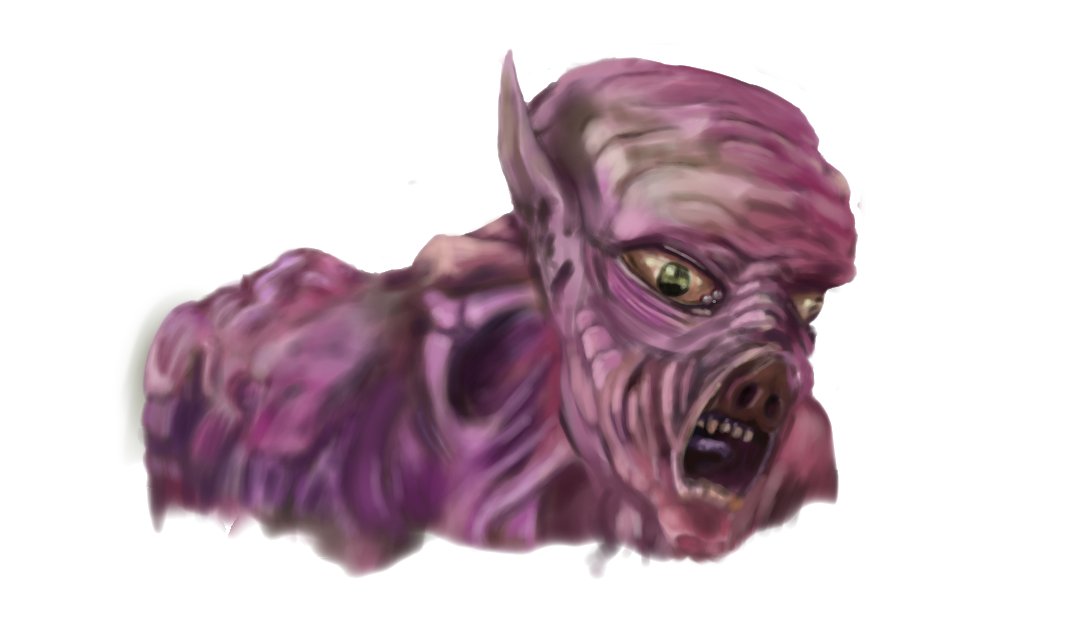
\includegraphics[width=8cm]{Pictures/witchghul.png}
		        %\caption{Witchghul}
             \label{fig:Witchghul}
        \end{figure}

Es ist wohl falsch von dem Ghul als eine stereotypischen Art zu sprechen. Die vielen Unterarten unterscheiden sich massivst in jeder Richtung und Form. Das einzige was sie Teilen ist der Drang zur Tat und dem Verlangen der Macht. Die Ghule werden in der Regel von dem Wohlhabensten angeführt. Meistens sind diese Kreaturen die mächtigen, scshlauen Witchghule. Ihre nekromantischen Fähigkeiten und ihre listigen Vorgehensweisen bringen sie immer wieder aus den Schatten ihrer größeren Brüder in das Rampenlicht und zu ihrer geliebten Beute. Die Kriegshorden der Ghule bestehen meist aus den großen Dork. Mit mindestens 2 Meter Höhe, riesigen Muskeln und ihrem grausam schlechten Musikgeschmack, sind die gröllenden Grauhäute mächtige Kriegswerkzeuge. Ihr Absolutes Gegenbild sind die chaotischen, werkelnden Orks. Sie basteln an riesigen Kriegsmaschinen und tragen die wundersamsten Maschinerien auf das Kampffeld. Wo der Dork mit Muskelkraft den Gegener niederschlägt, bezwingt der Ork seinen Gegenüber mit waghalsigen Ideen und der mangelnden Idee von Angst. Doch die Darstellung eines rein Kriegerischen Volks wäre ungerecht, da die vierte große Unterart, der Nork, eine sehr friedliche Gruppierung darstellt. Berühmt für ihren Eifer ihr fettiges sprödes Haar in den wildestens Formen zu präsentieren und zu pflegen, sind die Nord die Landwirte der Ghule. Sie pflanzen die berühmten Wimmerblüten, fertigen Kleidung und schreinern für den brutalen Rest.

\section*{Artenmerkmale}

\begin{tcolorbox}[title=Artenwerte,colbacktitle=myviolet,tabulars={@{\extracolsep{\fill}\hspace{5mm}}cccc@{\hspace{5mm}}},boxrule=0.5pt]
\textbf{Wunden} & \textbf{Gift} & \textbf{Psyche} & \textbf{Bewegung} \\\hline
        45 & 12 & 11 & 5 \\ \hlineB{3}
    \multicolumn{2}{ r| }{\textbf{Rasse:}} & \multicolumn{2}{ c }{Mischling} \\
    \multicolumn{2}{ r| }{\textbf{Größe:}} & \multicolumn{2}{ c }{Mittel, 1.5 - 2 m} \\
    \multicolumn{2}{ r| }{\textbf{Gewicht:}} & \multicolumn{2}{ c }{ 50 - 100 kg} 
\end{tcolorbox}

\subsection*{Genetik der Ghule}
\vspace*{0.75 cm}

\begin{tcolorbox}[title= Herz Genetik,colbacktitle=red, tabulars={@{\extracolsep{\fill}\hspace{5mm}}lc@{\hspace{1mm}}}, boxrule=0.5pt]
    \textbf{Rang 1:} & +2 auf Geschicklichkeit \\
    \textbf{Rang 2:} & +2 auf Sinne \\
    \textbf{Rang 3:} & +2 auf Gewandtheit \\
    \textbf{Rang 4:} & Aktion \verweis{sk:schlachtruf} \\
    \textbf{Rang 5:} & +4 auf Kreativität \\
\end{tcolorbox}
\vspace*{0.4 cm}

\begin{tcolorbox}[title= Pik Genetik,colbacktitle=gray, tabulars={@{\extracolsep{\fill}\hspace{5mm}}lc@{\hspace{1mm}}}, boxrule=0.5pt]
    \textbf{Rang 1:} & +2 auf Kraft \\
    \textbf{Rang 2:} & Aktion \verweis{sk:ueberwaeltigen} \\
    \textbf{Rang 3:} & +6 auf Wunden \\
    \textbf{Rang 4:} & +2 auf Gifte \\
    \textbf{Rang 5:} & +3 Robustheit \\
\end{tcolorbox}
\vspace*{0.4 cm}

\begin{tcolorbox}[title= Karo Genetik,colbacktitle=red, tabulars={@{\extracolsep{\fill}\hspace{5mm}}lc@{\hspace{1mm}}}, boxrule=0.5pt]
    \textbf{Rang 1:} & +1 im Element Tod \\
    \textbf{Rang 2:} & Aktion \verweis{sk:leichensucher} \\
    \textbf{Rang 3:} & +2 im Element Tod \\
    \textbf{Rang 4:} & +2 auf Spirit \\
    \textbf{Rang 5:} & Aktion \verweis{sk:beschwoerer} \\
\end{tcolorbox}
\vspace*{0.4 cm}

\begin{tcolorbox}[title= Kreuz Genetik,colbacktitle=gray, tabulars={@{\extracolsep{\fill}\hspace{5mm}}lc@{\hspace{1mm}}}, boxrule=0.5pt]
    \textbf{Rang 1:} & Aktion \verweis{sk:erstschlag} \\
    \textbf{Rang 2:} & +2 auf Initiative \\
    \textbf{Rang 3:} & +2 Waffenbonus auf Nahkampfwaffen \\
    \textbf{Rang 4:} & +3 Psyche \\
    \textbf{Rang 5:} & +1 Bewegung \\
\end{tcolorbox}

\subsection*{Grundzüge}
Auch wenn die Ghule sehr verschieden sind vereint sie doch ihre ursprüngliche Abstammung. Diese Abstammung gewärt ihnen immernoch primitive, aber dennoch sehr nützliche Vorteile.\\
Dein Charakter verfügt von beginn an über die Aktionen: \verweis{sk:wutanfall} und \verweis{sk:schmetterschlag}.

\subsection*{Schmetterschlag} \label{sk:schmetterschlag}
Mit einer mächtigen Bewegung nimmt der Ghul jegliche ihm zur Verfügung stehende Kraft zusammen und zwing seine rohe Waffe nieder gen Boden. Einem Regen aus Stahl, Blut und Stückchen zerschellt sie an dem triefende Aufprall am Gegner. \\
\textbf{Grundwert:} Kraft \\
\textbf{Kenntnisschwelle:} 2 \\
\textbf{Anforderungen:} $\Kreuz{}$ \\
\textbf{Reichweite:} 0.5 m \\
\textbf{Effekt:}  Lege eine Karte ab. \textit{Angriff (Physisch)}. Ignoriere die Rüstungs/Schild Bonis der Kreatur. Falls eine Waffe für diese Aktion verwendet wird Zerbricht diese (nur Nahkampfwaffen können genutzt werden), falls die oberste Karte ein Kreuz ist richtet dabei Wunden in Höhe des Bonuses an.

\subsection*{Wutanfall} \label{sk:wutanfall}
Emotionen spielen eine zentralle Rolle im Leben der Ghule. Sie lieben das Gefühl von Dominanz, sie hassen die Hilflosigkeit und sie können echt wütend werden. Eine solch wütende Kreatur in den Feindreihen zu sehen, bringt einen schnell dazu seine Pläne um zu ändern. \\
\textbf{Grundwert:} Emotionen \\
\textbf{Kenntnisschwelle:} 5 \\
\textbf{Anforderungen:} $\Herz{}$ 16+ \\
\textbf{Effekt:} \textit{Angriff (Psyche)}: Falls die Kreatur diese Aktionsrunde noch nicht dran war, kannst du dich entscheiden keinen Schaden zu machen, dafür muss die Kreatur in seiner nächsten Aktionsphase eine Vorausplannen Aktion durchführen. 


\begin{table}[h!]
    \centering
    \scalebox{0.95}{
    \begin{tabular}{|>{\columncolor[RGB]{247, 216, 212}}l|}
    \btrule{1pt}
    \arrayrulecolor{black}
    \\
    \textbf{\large Ghule}\\
    \\
        \begin{tabular}{c|c|c}
           \rowcolor{myred} \begin{tabular}{c}
               \rowcolor{myred}\textbf{Gefahren-}  \\
                \rowcolor{myred} \textbf{wert}\\ 
            \end{tabular} & \textbf{Fähingkeiten} & \textbf{Ausprägung}\\
            \hline
            \rowcolor{myred} 1. & -- & Herausforderung \\
            \rowcolor{myviolet} 2. & 1x Simpel & Herausforderung \\
            \rowcolor{myred} 3. & 1x Erweiter & Herausforderung\\
            \rowcolor{myviolet} 4. & 1x Komplex &  Körperentw. \\
            \rowcolor{myred} 5. & -- &  Herausforderung\\
            \rowcolor{myviolet} 6. & -- & Körperentw. \\
            \rowcolor{myred} 7. & 2x Simpel &  Herausforderung \\
            \rowcolor{myviolet} 8. & 2x Erweitert & Waffenbastler\\
            \rowcolor{myred} 9. & 1x Komplex & Herausforderung\\
            \rowcolor{myviolet} 10. & -- & Fährtenleser \\
            \rowcolor{myred} 11. & 1x Simpel & Charakterentw.\\
            \rowcolor{myviolet} 12. & 1x Simpel & Herausforderung\\
            \rowcolor{myred} 13. & 1x Erweitert & Körperentw.\\
            \rowcolor{myviolet} 14. & 1x Komplex & Waffenbastler\\
            \rowcolor{myred} 15. & -- & Herausforderung\\
            \rowcolor{myviolet} 16. & 1x Simpel & Charakterentw.\\
            \rowcolor{myred} 17. & 1x Erweitert  & Körperentw.\\
            \rowcolor{myviolet} 18. & 1x Erweitert & Herausforderung \\
            \rowcolor{myred} 19. & 1x Komplex & Waffenbastler\\
            \rowcolor{myviolet} 20. & -- & Körperentw.\\
            \rowcolor{myred} 21. & 2x Simpel & Körperentw.\\
            \rowcolor{myviolet} 22. & 1x Erweitert & Herausforderung\\
            \rowcolor{myred} 23. & 1x Komplex & Charakterentw.\\
            \rowcolor{myviolet} 24. & 1x Komplex & Körperentw.\\
            \rowcolor{myred} 25. & Gemeisterte Waffe & Waffenbastler \\
            %\rowcolor{myviolet} 26. & -- & Herausforderung\\
            %\rowcolor{myred} 27. & 2x Simpel & \\
            %\rowcolor{myviolet} 28. & 2x Erweitert& \\
            %\rowcolor{myred} 29. & 2x Komplex & \\
            %\rowcolor{myviolet} 30. &  (Spezifisch) & Herausforderung\\
        \end{tabular}\\
        \rowcolor{myred}\\
        \btrule{1pt}
    \end{tabular}}
\end{table}


\subsection*{Der Beginn des Ruhms}
Mit der Bestimmung der Körperattribute kommt für den Ghulspieler eine weiter Wahl: Seine Unterart. Besonders interessant kann für ihn hierbei die Anzahl der vor ihm liegenden Symbolen sein. Denn je nach den Anzahl der Symbole kann der Spieler Boni bekommen, siehe Genetik. Zur Wahl stehen die vier Völker der Norks, Dorks, Witchghule und Orks.

\section*{Herausforderungen der Völker}
Jedes der Ghulvölker hat seine eigenen Vorzüge und Kultur, damit gehen aber auch andere Herausforderungen einher, auf die sich die einzelnen Völker über Generationen spezialisiert haben.   

\subsection*{Waffenbastler} \label{sk:waffenbastler}
Mit ihrer ausgeprägten Kreativität, wie ihrem Talent im Handwerk ist es Ghulen meist ein leichtes Waffen zu erfinden oder zu verbessern. Wähle mit dem Erreichen der Gefahrenstuffe 8./14./19. \& 25. jeweils eine Verbesserung.\\
\begin{itemize}
    \item \textbf{Durchschlagen [I]:} \\
    Geschosse, wie auch Klingen durchschlagen besser Rüstung. Deine Waffe ignoriert Rüstung in Höhe ihres Waffenbonus.
    
    \item \textbf{Meisterhafte Waffe [I-IV]:}\\
    Auch wenn eine Waffe schon perfekt wirkt lässt sich immer noch etwas finden um die Waffe zu verbessern. Dein Waffenbonus erhöht sich um +3. Diese Verbesserung kann bis zu 4 mal gewählt werden.
    
    \item \textbf{Gift!! [I-III]} \\
    Vergiftet deine Waffe und fügt pro Rang zusätzlich Giftwunden in Höhe des Waffenbonus zu. 
    Diese Verbesserung kann bis zu 3mal gewählt werden.
    
    \item \textbf{Spiritmodul [I]} \\
    Ein Spiritmodul hilft dir mit der Waffe deine Spiritkrafte zu bündeln. Deine Waffenbonus kann nun auf jede Aktion mit Grundwert Spirit angerechnet werden. 
    
    \item \textbf{Lebensessenz [I-III]} \\
    Deine Waffen saugt das Leben deiner Feinde aus um dich zu heilen. Bei Angriffen mit deiner Waffe heile dich um 1/10 der verursachten Wunden. Erhöht sich auf 1/5 auf Rang II bis zu 1/2 auf Rang III. Diese Verbesserung kann bis zu 3 mal gewählt werden.  
\end{itemize}

\subsection*{Herausforderung der Norks $\Herz{}$}
\textbf{Boni:} Dein Gewandtheits- und Geschicklichkeitswert steigern sich mit +3, jedoch verringert sich dein Wundenwert um 3 \\
\textbf{Anfangsausrüstung:} Du startest mit \textit{einfacher Kleidung}, Zähnen im Wert von 80 + 2*Intelligenz EW, einem selbstgefertigten \verweis{ar:stichhaender}, welches in Absprache mit dem Spielmeister ein spezielles Merkmal haben kann und einem möglichen weiteren \textit{persönlichen Gegenständen}. \\
\textbf{Startfertigkeit:} \verweis{sk:rudelstärke}

\subsubsection*{\fbox{1} Gruppenstärke} \label{sk:gruppenstärke}
Ab Gefahrenwert 1 erhältst du die Passive Gruppenstärke.\\
\\
Der geschickteste Gruppenjäger der Welt weiß genau wie man als Gruppe zuzuschlagen hat. Die Jäger des Nordens kennen die effektivsten Strategien in jeder Situation um aus den Positionen ihrer Kameraden Vorteile zu ziehen. \\
\textbf{Effekt:} \textit{Passiv.} Bekomme für jede befreundete Kreatur die sich am Kampf beteiligt +1 auf Kraft oder Geschicklichkeit. \\
\textbf{Steigerung [15]:} Der Bonus Steigert sich auf +2.\\
\textbf{Steigerung [25]:} Der Bonus gilt nun für Kraft und Robustheit oder Geschicklichkeit und Gewandtheit.

\subsubsection*{\fbox{2} Waffenspezialist} \label{sk:waffenspezialist}
Ab Gefahrenwert 2 erhältst du die Passive Waffenspezialist.\\
\\
Nirgendwo in den Heimlichen Landen gibt es so perfektionistische Künstler des Klingentanzes wie es die Nord sind. Selbst mit den plumpen Waffen der Menschen können sie ihre Gegner alt aussehen lassen. \\
\textbf{Effekt:} \textit{Passiv.} Waffenbonis von deinen Waffen sind verdoppelt.\\
\textbf{Steigerung [15]:} Waffenbonis von deinen Waffen sind verdreifacht.

\subsubsection*{\fbox{3} Kultiviertes Töten} \label{sk:kultiviertes_töten}
Ab Gefahrenwert 3 erhältst du die Passive Kultiviertes Töten.\\
\\
Die Ehre der Nord verbietet es ihnen würdige Gegner bloß durch glückliche Treffer um zu bringen - schließlich wollen sie ja selber nicht im Duell gegen einen schwächeren Gegner fallen.\\
\textbf{Effekt:} \textit{Passiv.} Wann immer der Schaden, den du einer Kreatur zufügst, dem Gegner weniger als 5 Wunden übrig lässt, so muss sie ein Charismatest ablegen. Sollte sie sich stolz genug präsentiert (Test bestehen) stribt sie, ansonsten verbleibt sie mit übrigen 5 Wunden und \textit{blutet}(2).

\subsubsection*{\fbox{5} Athledisch} \label{sk:athledisch}
Ab Gefahrenwert 5 erhältst du die Passive Athledisch.\\
\\
Nach einer Weile der offensiven Urlaubsreisen entwickelt der Nork mit Stufe 5 einen athledischen Körpa.\\
\textbf{Boni:} Wann immer der Nork versucht sich gewaltsam durch seine Umgebung zu bewegen und hier für eine Probe notwendig ist, darf der Nork die aufgedeckte Karte ablegen und stattdessen ein zwei Karte ziehen, die er verwenden muss.

\subsubsection*{\fbox{7} Große Träume} \label{sk:große_Träume}
Ab Gefahrenwert 7 erhältst du die Passive Große Träume.\\
\\
Mit der Zeit beginnt ein jeder Nork seine geliebte Heimat zu vermissen. Wenn sich zwischen ihn und seine Rückkehr stellt wird das nicht gut ausgehen...\\
\textbf{Effekt:} \textit{passiv.} In Kämpfen (die dir unfreiwillig aufgezwungen wurden,) darfst du eine zusätzliche Karte auf die Hand ziehen. Lege wen du nur noch eine Karte auf der Hand hast diese sofort ab.

\subsubsection*{\fbox{9} Unbäugsam} \label{sk:unbäugsam}
Ab Gefahrenwert 9 erhältst du die Passive Unbäugsam.\\
\\
Die Willensstarken Nork sind in der Lage selbst in den gefährlichsten Situationen noch aufrecht zusammen zu stehen und nicht aufzugeben.\\
\textbf{Effekt:} \textit{passiv.} Reduziere psychischen Schaden pro kampfbereiten \textit{Freund} in deiner unmittelbaren Nähe (ca. 5 m) um 1.\\
\textbf{Steigerung [20]:} Pro kampfbereiten \textit{Freund} erhöht sich die Reduktion auf 2.

\subsubsection*{\fbox{12} Riposte} \label{sk:riposte}
Ab Gefahrenwert 12 erhältst du die Aktion Riposte.\\
\\
Gut trainiert mit deiner Waffe kannst du deine Verteidigung auch zu deinem Angriff machen. \\
\textbf{Grundwert:} Geschicklichkeit \\
\textbf{Kenntnisschwelle:} 2 \\
\textbf{Anforderungen:} $\Kreuz{}$ \\
\textbf{Reichweite:} Waffenreichweite \\
\textbf{Effekt:} \textit{Angriff (Physisch)}. Deine letzte Verteidigungskarte als Bonus. Kann nur gegen die Kreatur genutzt werden die dich zuletzt Angegriffen hat (innerhalb der Aktionsrunde). 

\subsubsection*{\fbox{15} Akt der Rache} \label{sk:aktderrache}
Ab Gefahrenwert 15 erhältst du die Passive Akt der Rache.\\
\\
Deine Instinkte verlangen von dir den Schutz deiner Familie und Freunde. So dürstet es dir instinktiv nach Rache falls einer von ihnen verletzt wird. \\
\textbf{Effekt:} \textit{passiv.} Wenn dein Ziel mit seiner letzten Aktion eine freundiche Kreatur Schaden zugefügt hat, erhältst du auf einen Angriff gegen diese Kreatur einen Bonus in Höhe der Wunden die sie verursacht hat.\\

\subsubsection*{\fbox{18} Furiose Angriffe} \label{sk:furioseangriffe}
Ab Gefahrenwert 18 erhältst du die Aktion Furiose Angriffe.\\
\\
Manchmal gerät auch ein Norks ausser Kontrolle und will alles was ihm nicht passt kleinhauen. \\
\textbf{Grundwert:} Geschicklichkeit \\
\textbf{Kenntnisschwelle:} 2 \\
\textbf{Anforderungen:} 22+ \\
\textbf{Reichweite:} Waffenreichweite \\
\textbf{Effekt:} \textit{Angriff (Physisch)}. Füge bis zu 4 verschiedenen Kreaturen Schaden zu, für jede Kreatur bekommst du auf deine nächste Verteidigung einen Malus von 5 (der Malus ist Aktions- wie auch Kampfrunden übergreifend).

\subsubsection*{\fbox{22} Feine Technik} \label{sk:feinetechnik}
Ab Gefahrenwert 22 erhältst du die Passive Feine Technik.\\
\\
Norks können auch noch mit stumpfen Waffen mithilfe ihrer jahrelangen perfektionierten Technik größen Schaden anrichten.\\
\textbf{Effekt:} \textit{passiv.} Anstelle des Waffenbonus der Waffe kannst du auch $\frac{Kraft+Geschick}{10}$ als Waffenbonus nutzen.\\

%####################################%

\subsection*{Herausforderung der Dorks $\Pik{}$}
\textbf{Boni:} Als Dorkspieler werden dein Kraftwert um 2 und dein Wundenwert um 10 erhöht. Zudem gehörst du der Größenortnung groß an. \\
\textbf{Anfangsausrüstung:} Du startest mit \textit{Schuppenpanzer}, \textit{einfacher Kleidung}, Zähnen im Wert von 80 + 2*Kraft EW, einer \verweis{ar:hiebwaffe} (+1) \textit{oder} einem \verweis{ar:bogen} (+1) und einem möglichen \textit{persönlichen Gegenständen}. \\
\textbf{Startfertigkeit:} \verweis{sk:fels_in_der_brandung}

\subsubsection*{\fbox{1} Fels in der Brandung} \label{sk:fels_in_der_brandung}
Ab Gefahrenwert 1 erhältst du die Aktion Fels in der Brandung.\\
\\
Mit einer triefenden Entschlossenheit stellt sich der riesige Dork seinen Widersachern. An ihm werden sie heute nicht vorbeikommen. \\
\textbf{Grundwert:} Willenskraft \\
\textbf{Kenntnisschwelle:} 5 \\
\textbf{Anforderungen:} Stationär \& $\Pik{}$ \\
\textbf{Reichweite:} 2 m \\
\textbf{Effekt:} Bis zu deiner nächsten Aktionsphase müssen Kreaturen die sich in Reichweite befinden eine vergleichende Probe gegen deinen Gesammtwert gewinnen um eine mit dir befreundete Kreatur als Ziel einer \textit{Angriffsaktion} wählen zu dürfen. Für die Dauer des Effekts steigt deine Robustheit um 1. 

\subsubsection*{\fbox{2} Überlaufen} \label{sk:überlaufen}
Ab Gefahrenwert 2 erhältst du die Passive Überlaufen.\\
\\
Mit Gefahrenstufe 2 weißt du wie du am besten Gegner über den Haufen rennst.\\ \\
Wie ein wildest Biest stürmt den Dork einfach durch den Pöbel hindurch. Die über bleibenden Reste bleiben den Orks zum auseinander nehmen übrig. \\
\textbf{Effekt:} \textit{Passiv}. In deiner Bewegung darfst du dich durch kleine Kreaturen durch bewegen. Solltest du am Ende der Bewegung mit ihnen Überlappen so werden sie hinreichend von dir wegbewegt um ein Wegrempeln widerzuspiegeln.\\
\textbf{Steigerung [15]:} Du kannst dich auch durch mittlere Kreaturen bewegen.

\subsubsection*{\fbox{3} Lauf'or Strib!} \label{sk:lauforstrib}
Ab Gefahrenwert 3 erhältst du die Passive Lauf'or Strib!\\
\\
Der reine Anblick eines Dorks kann sehr erschreckend sein. Die Vorstellung ihm zu missfallen noch viel mehr.\\
\textbf{Effekt:} \textit{passiv.} Kreaturen die kleiner sind als du und unter deinem Kommando stehen können deinen Kraftwert zum Verteidigen von psychischen Angriffen nutzen.

\subsubsection*{\fbox{5}Raserei} \label{sk:raserei}
Ab Gefahrenwert 5 erhältst du die Aktion Raserei.\\
\\
Die Wut die in den Herzen der Dorks brennen kann, ist die wohl bekannteste Emotionsregung dieser Muskelpakete. Wenn sie einmal in Rage fallen sind ihre Angriffe unglaublich brutal und tödlich. \\
\textbf{Grundwert:} Emotionen \\
\textbf{Kenntnisschwelle:} 8 \\
\textbf{Anforderungen:} $\Pik{}$ \\
\textbf{Effekt:} Für deine nächsten 1 + FK Aktionsphasen darfst du kostenfrei unterschiedliche Angriffsaktionen verketten.

\subsubsection*{\fbox{7} Vertraun} \label{sk:vertraun}
Ab Gefahrenwert 7 erhältst du die Passive Vertraun.\\
\\
Selbst der größte Knochen dieser Erde, kann nicht ewig stehen, wenn die Flut an Gegner an ihm nagt. Zwei Knochen können sich hingegen gegenseitig stützen.\\
\textbf{Effekt:} \textit{passiv.} Sind mehr Feinde als Freunde in deiner unmittelbaren Umgebung, erhalten deine Freunde +2 auf ihrer Körperattribute.

\subsubsection*{\fbox{9} Stahlbad} \label{sk:stahlbad}
Ab Gefahrenwert 8 erhältst du die Passive Stahlbad.\\
\\
Der feine Geruch und Kreischen von rostigen Stahl erfreut das Herz eines jeden Dorks. Bewegt man die Schulter einwenig rückwerts, dann kratzt da sogar etwas... Der Dork weiß wie er sich selbst motivieren kann um Vorteile zu kreieren.\\
\textbf{Effekt:} Du kannst deine metallische Ausrüstung so bewegen, dass du so richtig Lust bekommst weiter drauf rumzuhauen.

%####################################%

\subsection*{Herausforderung der Witchghule $\Karo{}$}
\textbf{Boni:} Du startest mit dem Merkmal \verweis{ef:element} Tod. Der Wert dieser Eigenschaft entspricht +2 \\
\textbf{Anfangsausrüstung:} Du startest mit \textit{einfacher Kleidung}, einem \verweis{ar:nekromantenstab} und deinen \textit{persönlichen Gegenständen}. \\
\textbf{Startfertigkeit:} \verweis{sk:organzerfall}

\subsubsection*{\fbox{1} Organzerfall} \label{sk:organzerfall}
Ab Gefahrenwert 1 erhältst du die Aktion Organzerfall.\\
\\
Opfer berichten von einem schmerzhaften Stechen in ihren Mägen, gefolgt von Blasenbildungen. Also bevor sie starben. Schmerzhaft. \\
\textbf{Grundwert:} Spirit \\
\textbf{Kenntnisschwelle:} 3 \\
\textbf{Maximale Kenntnis:} 10 \\
\textbf{Anforderungen:} $\Karo{}$ 15+ \\
\textbf{Reichweite:} 15 + FK m \\
\textbf{Effekt:} \textit{Angriff (Gift)}. \textbf{Bonus:} \textit{Element Tod} mal 2.

\subsubsection*{\fbox{2} Diener der Willkür} \label{sk:dienerderwillkür}
Ab Gefahrenwert 2 erhältst du die Passive Diener der Willkür.\\
\\
Kleine wilde Tiere, wie das gefräßige Knochhörnchen, begleiten gerne Witchghule da sie so leicht an eine Menge von toten Fleisch kommen und zu dem jemanden haben, der auf sie aufpasst.
\textbf{Kenntnisschwelle:} 1 \\
\textbf{Maximale Kenntnis:} 10 \\
\textbf{Effekt:} Du hast Besitz über ein kleines Wesen, welches dir als kleiner Begleiter fungiert. Es wird jedoch panisch vor Kämpfen. \\
\textbf{Steigerung [5]:} Das Wesen ist in der Lage kleinere Gegenstände zu dir zu bringen und Spuren auf zu nehmen. Es versteht simple Befehle.(Sollte jetzt auch Kämpfen können) \\
\textbf{Steigerung [10]:} Du kennst das Wesen mittlerweile so gut, dass du sein Verhalten deuten kannst und du es z.B. als Späher nutzt kannst.

\subsubsection*{\fbox{3} Leichenexplosion} \label{sk:leichenexplosion}
Ab Gefahrenwert 3 erhältst du die Aktion Leichenexplosion.\\
\\
Einer der vielen Gründen warum Witchghule von verschiedensten Lebensformen gehasst werden, ist ihr mangelnder Respekt vor Toten. Besonders abartig sind die blutgetränkten Explosionen ihrer toten Feinde und Freunde, deren Knochensplittern umstehende Opfer durchbohren. \\
\textbf{Grundwert:} Spirit \\
\textbf{Kenntnisschwelle:} 2 \\
\textbf{Maximale Kenntnis:} 5 \\
\textbf{Anforderungen:} 25+ \\
\textbf{Reichweite:} 6 + FK m \\
\textbf{Effekt:} Wähle eine Leiche in Reichweite. Im Radius von \textbf{FK} m um die Leiche erleiden alle Kreaturen \textbf{GW} Schaden. Sollte die Leiche noch nicht tot sein, so erleidet sie ernst zu nehmenden Schaden. Dieser beträgt die Hälfte ihrer maximalen Wunden.

\subsubsection*{\fbox{5} Beschwörer} \label{sk:beschwoerer}
Ab Gefahrenwert 5 erhältst du die Passive Beschwörer.\\
\\
Eine erfolgreiche Witchghulekarriere hängt mit vielerlei Faktoren zusammen. Eine wichtige Schlüsselstelle markiert jedoch defenitiv der Umgang mit minderen Kreaturen. Ist man zu streng muss man sie zuhäufig wiederbeleben, ist man zu lasch so entwickeln sie positive Emotionen. \\
\textbf{Effekt:} \textit{Passiv.} Untergebene Kreaturen haben +7 Wunden und +2 auf alle Körpereigenschaften.

\subsubsection*{\fbox{7} Leichensucher} \label{sk:leichensucher}
Ab Gefahrenwert 7 erhältst du die Aktion Leichensucher.\\
\\
Um ihre nekromantischen Fähigkeiten zu erproben, lernt der Witchghule bereits in früh, wie er möglichst effektiv seinen Sinn auf der Suche nach Leichen einsetzen kann. \\
\textbf{Kenntnisschwelle:} 2 \\
\textbf{Maximale Kenntnis:} 15 \\
\textbf{Reichweite:} 5 + FK m \\
\textbf{Effekt:} Du kannst Tote innerhalb der Reichweite aufspüren, selbst wenn sie schon lange begrabene, verwesende Geschöpfe sind. Du kannst sie vereinfacht ausgraben (+2) und sie wenn möglich gut identifizieren (+2).\\
\textbf{Steigerung [15]:}Du kannst sie noch vereinfachter ausgraben +5 und sie besser identifizieren +5.

\subsubsection*{\fbox{9} Rituale der Witchghule} \label{sk:ritualederwitchghule}
Ab Gefahrenwert 9 erhältst du die Aktion Rituale der Witchghule.\\
\\
Die Rituale der Witchghule sind hohe Kunst der Nekromantie und lassen manch eine Seele wieder in die Welt zurückkehren. \\
\textbf{Grundwert:} Spirit \\
\textbf{Kenntnisschwelle:} 2 \\
\textbf{Maximale Kenntnis:} 7 \\
\textbf{Anforderungen:} $\Karo{}$ \& 20+ \\
\textbf{Reichweite:} Berührung \\
\textbf{Effekt:} Du kannst noch relativ frische Leichen zu einer einfachen Ghulbrut (Zombie) wiederbeleben. Das Talent gewährt dir die Kontrolle über einen Untoten gleichzeitig zu haben.\\
\textbf{Steigerung [15]:} Du kannst altere Leichen und Skelette zurück in lebende Welt holen als Ghulsöldner.

\subsubsection*{\fbox{12} Nekrosis} \label{sk:nekrosis}
Ab Gefahrenwert 12 erhältst du die Aktion Nekrosis.\\
\\
Du regst den Körper des Ziels zum zerfall an. \\
\textbf{Grundwert:} Spirit \\
\textbf{Kenntnisschwelle:} 2 \\
\textbf{Maximale Kenntnis:} 5 \\
\textbf{Anforderungen:} $\Karo{}$ 20+ \\
\textbf{Reichweite:} 15 + FK m \\
\textbf{Effekt:} \textit{Angriff (Gift)}. \textbf{Bonus:} \textit{Element Tod}. Das Ziel kann diese Runde kein Gift abbauen.

\subsubsection*{\fbox{15} Giftgabe} \label{sk:giftgabe}
Ab Gefahrenwert 15 erhältst du die Passive Giftgabe.\\
\\
Neben der Nekromantie kennen sich die Witchghule auch bessonders gut mit Giften aus man könnte sagen sie hätten eine Gabe des Gifts. \\
\textbf{Effekt:} \textit{Passiv.} Wähle ein Gift als deine Gabe aus. Wann immer du jemanden Vergiftest kannst du anstelle eines Zufälligen Giftes das Gift auf ihn wirken. Die stärke der Vergiftungen die du wirkst ist verdoppelt.

\subsubsection*{\fbox{18} Das vergessene Rituale der Witchghule} \label{sk:leichensucher}
Ab Gefahrenwert 18 erhältst du die Aktion Das vergessene Rituale der Witchghule.\\
\\
Das vergessene Rituale der Witchghule ist die Spitze des Eisberges der Nekromantie. Es hat nichts mehr mit der Bindung einer Seele an einen Körper zu tun, sonder ist die Beschwörung einer leeren, willenlosen Abscheulichkeit. \\
\textbf{Grundwert:} Spirit \\
\textbf{Kenntnisschwelle:} 2 \\
\textbf{Maximale Kenntnis:} 5 \\
\textbf{Anforderungen:} $\Karo{}$ \& 25+ \\
\textbf{Reichweite:} In der nähe \\
\textbf{Effekt:} Aus einem Haufen aus Leichen ist es dir mit etwas Zeit möglich eine Abscheuslichkeit  zu beschwören.

\subsubsection*{\fbox{22} Flickwerk} \label{sk:flickwerk}
Ab Gefahrenwert 22 erhältst du die Passive Flickwerk.\\
\\
........... \\
\textbf{Effekt:} \textit{Passiv.} Du kannst dich mit deinen untoten Kreaturen verstärken, so dass du. Die Hälfte des Wundenlimits als temporer zunzubekommst, wie auch den höheren der jeweiligen Körperlichen Eigenschaften. So ballt die Zusatzwunden überschritten wurden verlierst du den Effekt.

%####################################%

\subsection*{Herausforderung der Orks $\Kreuz{}$}
\textbf{Boni:} Deine Initiative steigt um 5 und bei Gleichstand im Initiativzug erhälst du den Vorrang, jedoch verringert sich deinen Psyche um 2. Waffenbastler gilt auch für Granaten.\\
\textbf{Anfangsausrüstung:} Du startest mit \textit{einfacher Kleidung}, \textit{einfacher Kleidung} einer \verweis{ar:hiebwaffe} oder \textit{Werkzeug} und deinen \textit{persönlichen Gegenständen}. \\
\textbf{Startfertigkeit:} \verweis{sk:werkeln}.

\subsubsection*{\fbox{1} Werkeln} \label{sk:werkeln}
Nicht einmal der Mensch ist so innovativ wie der Ork. Seine Lust aufs Rumbasteln, schrauben und stanzen ist unaufhaltsam. Er kann in jeder Situation ein Gegenstand nehmen und wild mit ihm herum werkeln, bis er etwas aufregend Neues kann.\\
\textbf{Grundwert:} Kreativität oder Intelligenz \\
\textbf{Kenntnisschwelle:} 2 \\
\textbf{Anforderung:} Stationär \& 17+ \\
\textbf{Reichweite:} 1 m \\
\textbf{Effekt:} Bastel aus einer improvisierten Waffe eine \verweis{ar:hiebwaffe}\textit{[+1]} oder stelle bei Mrots FK Wunden wieder her. Es werden \textit{Werkzeuge} und ggf. Ersatzteile benötigt.

\subsubsection*{\fbox{2} Cnacka herstellen} \label{sk:cnacka_herstellen}
Ab Gefahrenwert 2 realisiert der Ork wie gefährlich das Herstellen von Cnackas doch sein kann.\\
\\
Schon im Kleinalter beginnen die Orks mit explosiven Pulvern und Behältern zu spielen. Im Laufe ihres Erwachsen werdens, verstehen sie die \verweis{ar:cnacka} richtig böse herzustellen.\\
\textbf{Effekt:} \textit{Passiv.} Du bist in der Lage aus \textit{explosiven Pulver}, einem \textit{Zundstein} und einem passenden Behälter \verweis{ar:cnacka} herzustellen. Führe hierzu eine Kreativitäsprobe durch. Solltest du dein Gegenzeichen als Bild aufdecken explodiert der \verweis{ar:cnacka} in deiner Hand. Dies ist auch im Kampf möglich.

\subsubsection*{\fbox{3} Schnotzenbratzer} \label{sk:schnotzenbratzer}
Mit Gefahrenwert 3 darfst du dein Ork ein Schnotzenbratzer nennen.\\
\\
Unter den Ghule kursiert die Bezeichnung des Schnotzenbratzer. Mit dieser werden die bekannte Orkschützen bezeichnet. Statt nur ihre Mrots in Stand zu halten tragen sie ihre gebastelten Gebärte (Gewehre) in den Kampf um ihre Feinde hinterrücks zu erschießen.\\
\textbf{Effekt:} \textit{Passiv.} Du bist in der Lage aus eines \textit{Stahlfeder} und einem Haufen Schrott dir dein eigenes \verweis{ar:gebärt} herzustellen. Da nur du weißt wie es funktioniert, kannst auch nur du es nutzen und bedienen. 

\subsubsection*{\fbox{5} Takdisha Kumpan} \label{sk:Takdisha_Kumpan}
Ab dem Gefahrenwert 5 begleitet den Ork ein Takdisha Kumpan.\\
\\
Orks basteln während ihrer Kariere sich gerne Begleiter. Die simpelste Form ist ein Takdisha Kumpan. Eine zweibeinige Blechbüxe der man in der Regel ein Geschütz oder eine Truhe einbaut.\\
\textbf{Effekt:} \textit{Passiv.} Dich begleitet ein \textit{Takdisha Kumpan} mit einer austauschbaren Truhe.
 
\subsubsection*{\fbox{7} Kabuuuum!} \label{sk:kabuuuum!}
Ab dem Gefahrenwert 7 kannst du die Aktion Kabuuuum! \\
\\
Mit Hilfe eines kleinen selbst geschraubten Geräts, kannst du mechanische Kreaturen zum Überladen bringen und somit explodieren lassen.\\
\textbf{Grundwert:} Kreativität \\
\textbf{Kenntnisschwelle:} 5 \\
\textbf{Anforderungen:} Stationär \& $\Kreuz{}$ \\
\textbf{Reichweite:} 8 m \\
\textbf{Effekt:} Wähle eine mechanische Kreatur, sollte die Kreatur noch leben, so kann sie sich mit mentalem Widerstand Verteidigen. Die gewählte Kreatur erleidet doppelte Wunden. Kreaturen iin einem 5 m Radius um die Kreatur erleiden durch die Explosion ebenfalls Schaden.  

\subsubsection*{\fbox{9} Megarbum} \label{sk:megarbum}
Ab dem Gefahrenwert 9 kannst du die Passive Megarbum \\
\\
Nach dem treuen Motto je stärker die Bombe desto besser, sind nur die Explosionen, für die du natürlich "nicht" verantwortlich bist etwas stärker. \\
\textbf{Effekt:} \textit{Passiv.} Schaden durch Explosionen ist um +10 erhöht.\\
\textbf{Steigerung [9]:} Explosionsschaden um weitere +10 erhöht.

\subsubsection*{\fbox{12} Taschen Granate} \label{sk:taschengranate!}
Ab dem Gefahrenwert 12 kannst du die Aktion Taschen Granate. \\
\\
Es hilf immer eine Granate im Ärmel zu haben oder was es doch As.\\
\textbf{Grundwert:} Kreativität \\
\textbf{Kenntnisschwelle:} 2 \\
\textbf{Anforderungen:} $\Kreuz{}$ \\
\textbf{Reichweite:} 10 m \\
\textbf{Effekt:} \textit{Angriff (Physisch)}. Trifft alle im Radius von 3m um das getroffene Ziel.

\subsubsection*{\fbox{15} Großes BUM-BUM} \label{sk:GrosesBUMBUM}
Ab dem Gefahrenwert 15 kannst du die Passive Großes BUM-BUM. \\
\\
Du lässt es nun so richtig krachen und lädst gerne mehr Teilnehmer zum Experiment ein.\\
\textbf{Effekt:} \textit{Passiv.} Der Radius deiner Explosionen ist verdoppelt.

\subsubsection*{\fbox{18} Artillerie} \label{sk:artillerie!}
Ab dem Gefahrenwert 18 kannst du die Aktion Atillerie. \\
\\
Granaten zu werfen ist gut, weiter zu werfen ist besser.\\
\textbf{Grundwert:} Kreativität \\
\textbf{Kenntnisschwelle:} 2 \\
\textbf{Anforderungen:} $\Pik{}$ \\
\textbf{Reichweite:} ST +20 m \\
\textbf{Effekt:} \textit{Angriff (Physisch)}. Lege eine Karte ab. Trifft alle im Radius von 3m um das getroffene Ziel.

\subsubsection*{\fbox{22} Grenadier} \label{sk:Grenafier}
Ab dem Gefahrenwert 22 kannst du die Passive Grenadier. \\
\\
Du lässt die Granaten nur so fliegen.\\
\textbf{Effekt:} \textit{Passiv.} Du kannst zwei Granaten gleichzeitig Werfen, die Ziele dürfen nur 5m auseinander Stehen. Aktion in denen du Granaten wirfst, wirst du nun Automatisch 2.  

\subsection*{Für Reichtum und Wohlstand}
Um mehr Spannung ins Spiel zu bringen kann der Spielmeister sich in Absprache mit dem/den Guhlspieler/n dazu entscheiden, die Herausforderungen der einzelnen Völker auch wirklich als Herausforderung zu gestallten. Dabei bekommt der Spieler nicht direkt den Bonus des Volkes nach dem Erreichen eines neuen Gefahrenwertes, sondern erst eine Nebenquest mit dem Bonus und vielleicht etwas Loot als Belohnung.
Die Nebenquest sollte passend zum Bonus gewählt werden und gut/schnell machbar sein um Frust zu vermeiden. Sollte die alte Herausforderung noch nicht gemeistert worden sein, wenn er einen Gefahrenwert aufsteigt, so ist es möglich beliebig viel Herausforderungen parallel zu verfolgen.

\subsection*{Gemeisterte Waffe} \label{sk:gemeistertewaffe}
Als Waffenmeister gelangen Ghule irgendwann dazu ihre Waffe in und auswendig zu kennen.  \\
\textbf{Effekt:} \textit{Passiv.} Wahle einen Waffentypen. Du kannst Sonderbedingungen zu Nutzung von Waffen dessen Typs ignorieren (Zweihandwaffen benötigen jedoch immer noch zwei Hände). Du erhältst ebenso einen extra Waffenbonus von +5 auf Waffen des Typs.  

\subsection*{Ghulnamen:}

\subsubsection*{männlich:}
Graklas, Murkat der Steinschmeisser

% = = = = = = = = = = = = = = = = %

\clearpage

\section{Krograg} \label{art:krograg}

\begin{figure}[htbp]
        \centering
		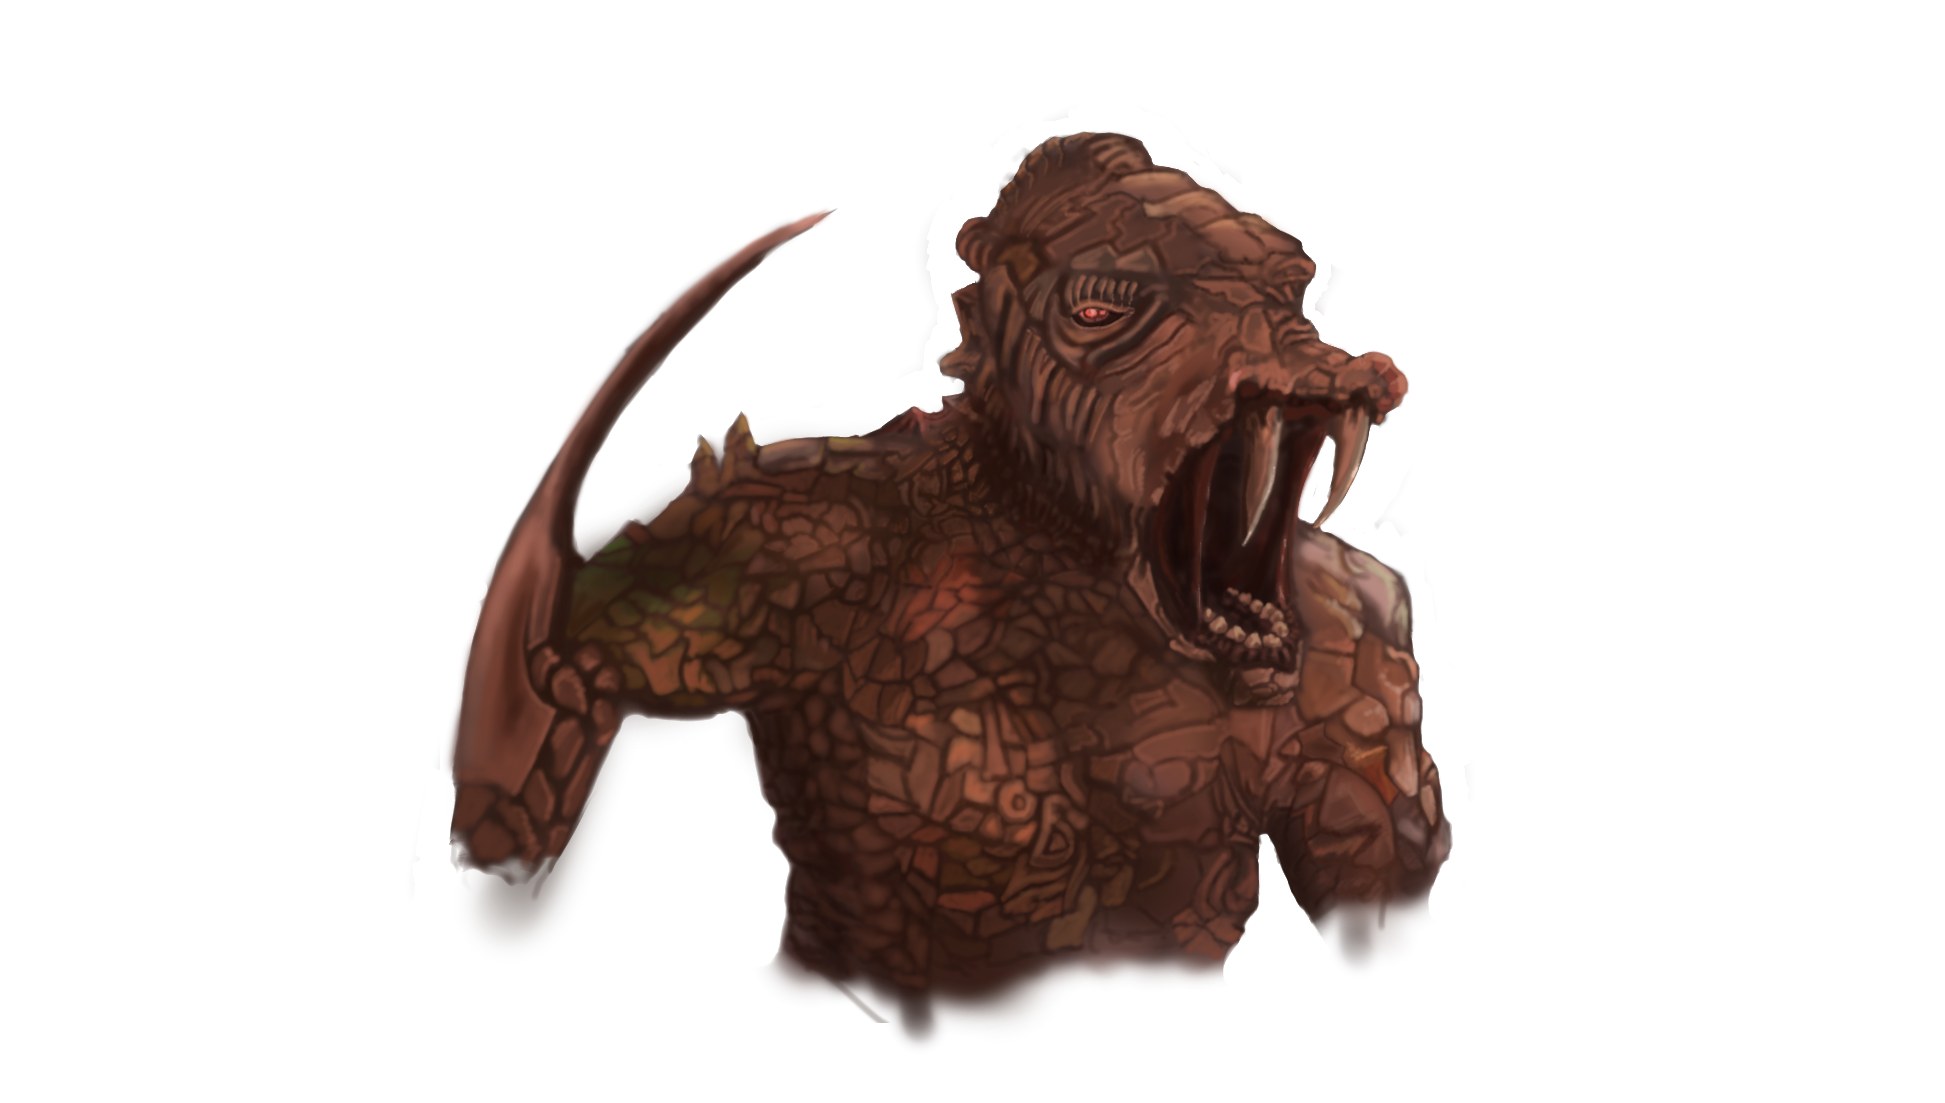
\includegraphics[width=8cm]{Pictures/Krograd.png}
        \label{fig:Krograg}
\end{figure}

Die Diener der 9 Schöpfer erlangen ihre Kraft aus ihrem Glauben. Die meisten Gebete der Schuppenhäutigen gehen an Varki (\textit{Schwester der Wüstel}), Moarln (\textit{Knüpfer der Netze}), Keark (\textit{Anwälter der Stränge}) und seine Schwester Kearkii (\textit{Mutter der Zeichen}). Einem jeden wurden unzählige kleinere Tempel und eine Hand voll Meaen (\textit{Hallen}) errichtet um ihre Zulassung zur Fortexistenz zu erhalten. Doch das Leben bietet einem guten Gläubigen auch die Möglichkeit einem zweiten Schöpfer seine Gedanken zu schenken. So bietet die Tochter der Feuchtigkeit Serkji, der Gefährte der Bewegung Nierld, die Läuterer der Heimat Aivir und die Gräfin der Ruhe Vand eine Möglichkeit sich dem Glauben zu beweisen. Dem letzten Schöpfer Prjalvad, Verführer der Ungewissheit verschreibt sich keine klar keine Denkende Kreatur. Ein jeder kennt die Geschichten um Hubert dem Hirnlosen und wird es ihm nicht gleich tun wollen.

\section*{Artenmerkmale}

\begin{tcolorbox}[title=Artenwerte,colbacktitle=mybrown,tabulars={@{\extracolsep{\fill}\hspace{5mm}}cccc@{\hspace{5mm}}},boxrule=0.5pt]
\textbf{Wunden} & \textbf{Gift} & \textbf{Psyche} & \textbf{Bewegung} \\\hline
        47 & 13 & 16 & 5 \\ \hlineB{3}
    \multicolumn{2}{ r| }{\textbf{Rasse:}} & \multicolumn{2}{ c }{Kratzer} \\
    \multicolumn{2}{ r| }{\textbf{Größe:}} & \multicolumn{2}{ c }{Mittel, 1.7 - 1.9 m} \\
    \multicolumn{2}{ r| }{\textbf{Gewicht:}} & \multicolumn{2}{ c }{ 65 - 120 kg} 
        \end{tcolorbox}
\subsection*{Genetik der Krograg}
\vspace*{0.75 cm}

\begin{tcolorbox}[title= Herz Genetik, colbacktitle=red, tabulars={@{\extracolsep{\fill}\hspace{5mm}}lc@{\hspace{1mm}}}, boxrule=0.5pt]
    \textbf{Rang 1:} & +2 auf Geschicklichkeit \\
    \textbf{Rang 2:} & +2 auf Willenskraft \\
    \textbf{Rang 3:} & Aktion \verweis{sk:rage} \\
    \textbf{Rang 4:} & +3 Emotion \\
    \textbf{Rang 5:} & +4 Gewandtheit \\
\end{tcolorbox}
\vspace*{0.4 cm}

\begin{tcolorbox}[title= Pik Genetik,colbacktitle=gray, tabulars={@{\extracolsep{\fill}\hspace{5mm}}lc@{\hspace{1mm}}}, boxrule=0.5pt]
    \textbf{Rang 1:} & +2 auf Robustheit \\
    \textbf{Rang 2:} & Aktion \verweis{sk:wasserbinden} \\
    \textbf{Rang 3:} & +2 auf Kraft\\
    \textbf{Rang 4:} & Aktion \verweis{sk:durchdringender_biss}\\
    \textbf{Rang 5:} & +3 auf Bissangriffe \\
\end{tcolorbox}
\vspace*{0.4 cm}

\begin{tcolorbox}[title= Karo Genetik,colbacktitle=red, tabulars={@{\extracolsep{\fill}\hspace{5mm}}lc@{\hspace{1mm}}}, boxrule=0.5pt]
    \textbf{Rang 1:} & +2 auf Spirit \\
    \textbf{Rang 2:} & Aktion \verweis{sk:sandsturm} \\
    \textbf{Rang 3:} & +2 auf Willenskraft \\
    \textbf{Rang 4:} & +3 Kreativität \\
    \textbf{Rang 5:} & Passive \verweis{sk:spiritfluss} \\
\end{tcolorbox}
\vspace*{0.4 cm}

\begin{tcolorbox}[title= Kreuz Genetik,colbacktitle=gray, tabulars={@{\extracolsep{\fill}\hspace{5mm}}lc@{\hspace{1mm}}}, boxrule=0.5pt]
    \textbf{Rang 1:} & +2 auf Wundenmaximum \\
    \textbf{Rang 2:} & +2  Toxin \\
    \textbf{Rang 3:} & Aktion \verweis{sk:duesterer_schlag} \\
    \textbf{Rang 4:} & +2 Waffenbonus \\
    \textbf{Rang 5:} & +5 Psyche \\
\end{tcolorbox}

\subsection*{Grundzüge}
Durch ihre Abstammung von Reptilien erhalten Krogrags nicht bloß das Merkmal \verweis{ef:schwimmer}, sondern sind auch in der Lage für bis zu einer halben Stunde unter Wasser zu bleiben.\\
Dein Charakter verfügt von beginn an über die Aktionen: \verweis{sk:kratzer} und \verweis{sk:spiritox_biss} , sowie die Passive: \verweis{sk:glaeubiger}.      


\subsection*{Gläubiger} \label{sk:glaeubiger}
Dein Leben ist eine Reise unter dem Schutz deines Schöpfers. Du kannst im Kampf jeder Zeit eine Karte opfern um ein \textit{Glaubenspunkt} zu kreieren. Deine Glaubenspunkte verfallen am Ende des Kampfes. Geistige Beeinträchtigungen lassen dich an deinen Glauben zweifeln und führen zu einer kurzzeitigen Schwächung deiner Kräfte. \\
\textbf{Effekt:} \textit{Passiv.} Solange du geistig umnachtet bist erhältst du je nach deiner Hauptgottheit einen Malus. \textbf{Keark:} du kannst die Aktion Ausweichen nicht nutzen, \textbf{Kearkii:} deine Rüstung wird halbiert, \textbf{Varkis:} deine Heilungseffekte heilen nur noch die Hälfte, \textbf{Moarln:} du verlierst deinen Waffenbonus und erhältst -5 auf Angriffe.

\subsection*{Kratzen} \label{sk:kratzer}
Mit einem flinken Bewegung fahren die Krallen der Krograg in das ungeschützte Fleisch ihrer Ziele. Mit agilen Bewegung setzt sie der saftigen Nahrung nach und lässt nicht nach bis sie das Fleisch im Munde spürt.\\
\textbf{Grundwert:} Geschicklichkeit \\
\textbf{Kenntnisschwelle:} 1 \\
\textbf{Maximale Kenntnis:} 15 \\
\textbf{Anforderungen:} Bewegend $\Herz{}$ \\
\textbf{Reichweite:} 1 m \\
\textbf{Effekt:} \textit{Angriff (Physisch)[X]}. Du kannst diese Aktion ohne Kosten mit sich selbst verketten. (Verkettung erfordert kein Herz)

\subsection*{Spiritox Biss} \label{sk:spiritox_biss}
Mit einer klebrigen Giftmischung in dem Zahninneren, kann der Krograt diese aggressive Flüssigkeit in dem Körper seines Gegners freisetzen.\\
\textbf{Grundwert:} Spirit \\
\textbf{Kenntnisschwelle:} 2 \\
\textbf{Anforderungen:} $\Karo{}$ 18+ \\
\textbf{Reichweite:} 0.5 m \\
\textbf{Effekt:} \textit{Angriff (Gift)}. Falls das Ziel durch diesen Angriff vergiftet wurde erleidet es zusätzlich \textbf{FK} Wunden.


\begin{table}[h!]
    \centering
    \begin{tabular}{|>{\columncolor[RGB]{247, 216, 212}}l|}
    \btrule{1pt}
    \arrayrulecolor{black}
    \\
    \textbf{\large Krograg}\\
    \\
        \begin{tabular}{c|c|c}
           \rowcolor{myred} \begin{tabular}{c}
               \rowcolor{myred}\textbf{Gefahren-}  \\
                \rowcolor{myred} \textbf{wert}\\ 
            \end{tabular} & \textbf{Fähingkeiten} & \textbf{Ausprägung}\\
            \hline
            \rowcolor{myred} 1. & -- & Glauben \\
            \rowcolor{mybrown} 2. & 1x Simpelt & Glauben \\
            \rowcolor{myred} 3. & 1x Erweiter & Glauben\\
            \rowcolor{mybrown} 4. & 1x Komplex &  Körperentw. \\
            \rowcolor{myred} 5. & (Spezifisch) &  Glauben\\
            \rowcolor{mybrown} 6. & -- & Charakterentw. \\
            \rowcolor{myred} 7. & 2x Simpel &  Glauben \\
            \rowcolor{mybrown} 8. & 1x Erweitert & (Spezifisch)\\
            \rowcolor{myred} 9. & 1x Komplex & Glauben\\
            \rowcolor{mybrown} 10. & (Spezifisch) & (Speuifisch) \\
            \rowcolor{myred} 11. & -- & Körperentw.\\
            \rowcolor{mybrown} 12. & 1x Simpel & Glauben\\
            \rowcolor{myred} 13. & 2x Erweitert & Körperentw.\\
            \rowcolor{mybrown} 14. & 1x Komplex & (Spezifisch)\\
            \rowcolor{myred} 15. & (Spezifisch) & Glauben\\
            \rowcolor{mybrown} 16. & -- & Charakterentw.\\
            \rowcolor{myred} 17. & 1x Simpel & Körperentw.\\
            \rowcolor{mybrown} 18. & 1x Erweitert & Glauben \\
            \rowcolor{myred} 19. & 2x Komplex & (Spezifisch)\\
            \rowcolor{mybrown} 20. & (Spezifisch) & Charakterentw.\\
            \rowcolor{myred} 21. & -- & Körperentw.\\
            \rowcolor{mybrown} 22. & 2x Simpel & Glauben\\
            \rowcolor{myred} 23. & 2x Erweitert & Körperentw.\\
            \rowcolor{mybrown} 24. & 2x Komplex & Charakterentw.\\
            \rowcolor{myred} 25. & (Spezifisch) & (Spezifisch) \\
            %\rowcolor{myblue} 26. & -- & Pfad\\
            %\rowcolor{myred} 27. & 2x Simpel & \\
            %\rowcolor{myblue} 28. & 2x Erweitert& \\
            %\rowcolor{myred} 29. & 2x Komplex & \\
            %\rowcolor{myblue} 30. &  (Spezifisch) & Pfad\\
        \end{tabular}\\
        \rowcolor{myred}\\
        \btrule{1pt}
    \end{tabular}
\end{table}

 

\section*{Glaubensrichtungen}
Ein jeder Krograg verschreibt sich einem der vier Götter Keark, Kearkii, Varkis oder Moarln zu dienen. Die Dienste bereiten nicht nur ein erfülltes Leben, sondern gewähren auch erstaunliche Fähigkeiten von denen andere Arten zu Träumen vermögen.    

\subsection*{Die Dienste Keark $\Herz{}$}
Diener von Keark halten sich im Verborgenen und wahren die Strukturen ihres Glauben auch wenn es nie jemand wissen wird. Häufig besteht ihre Aufgabe darin Informationen Gefangenen zu entlocken und sie anschließend ihrem Schöpfer näher zu bringen. Manchen wird die Aufgabe eines Dranraks zuteil. Dranraks sind elitäre Attentäter, die nach ihrem ermessen in Namen von Keark töten dürfen. Ihre Ziele finden in der Regel ihr Ende an einem frei schwingenden Strick. \\
\textbf{Boni:} \\
\textbf{Anfangsausrüstung:} \textit{Einfache Kleidung}, Strick, \textit{\nameref{ar:hiebwaffe}} [0.25 m, +1], Symbol des Kearks und deine \textit{persönliche Ausrüstung}  \\
\textbf{Startfähigkeit:} \verweis{sk:quaeler} \\

\subsubsection*{Quäler} \label{sk:quaeler}
Als Meister der Furcht sind Diener von Keark wahre Beherrscher der Unterdrückung und Psychologischenkriegsführung.\\
\textbf{Effekt:} Psychewunden, die du zugefügt hast, bekommen einen Bonus von +5.\\
\textbf{Steigerung [15]:} Der Bonus Steigert sich auf +10. \\
\textbf{Steigerung [25]:} Psychewunden, die du zufügst verdoppeln sich, der vorherige Bonus gilt nicht mehr.
\\
\\
Die nächsten Glaubensausprägungen dürfen frei aus den folgenden gewählt werden:

\subsubsection*{Schattenschlinge} \label{sk:schattenklinge}
Der Abend war ruhig, die Temperaturen kühl und die Sonne wenige Dolche vorm Untergehen. Alles war gut. Naja, bis auf die Schlinge die ihn überraschend in die Höhe zog. Die war gar nicht gut.\\
\textbf{Grundwert:} Geschicklichkeit + Kraft - gegn. Sinne \\
\textbf{Kenntnisschwelle:} 3 \\
\textbf{Anforderungen:} $\Karo{}$ \\
\textbf{Reichweite:} 0.5 m \\
\textbf{Effekt:} \textit{Angriff (Physisch)}. Wähle ein Ziel das sich bis zu 5 Meter unter dir befindet und maximal mittel groß ist. Es darf dich noch nicht wahrgenommen haben. Solltest du ihm Schaden machen, kannst du die schlinge weiterhin festhalten oder irgendwo befestigen. Wenn sich dein Opfer in der seiner nächsten Aktionsphase nicht befreit hat, verliert es die Hälfte seines verbleibenden Lebens. Dies gilt auch für die folgende Phase. In der dritten Leidensphase stirbt es.

\subsection*{Lauern} \label{sk:lauern}
Eine beliebte Jagdtaktik der Jäger des großen Kearks ist das überraschende Angreifen aus verborgenen Höhlen, Gruben oder Gestrüpp. Um einen Gegner derartig überrumpeln zu können benötigt es eine gutes Zeitgefühl und ein wenig Zeit zur Vorbereitung.\\
\textbf{Grundwert:} Geschicklichkeit \\
\textbf{Kenntnisschwelle:} 2 \\
\textbf{Anforderungen:} Stationär \\
\textbf{Reichweite:} 1 m \\
\textbf{Effekt:} \textit{Angriff (Physisch)}. Um diesen Angriff durchzuführen darfst du dich in der vorherigen Runde nicht Bewegt haben und momentan nicht im Nahkampf sein. Decke nachdem du deine Angriffskarte gespielt hast zwei Karten deines Decks auf und wähle von den drei Karten eine aus mit der du den Angriff ausführen möchtest.


Dranrak?


\subsection*{Die Dienste Varki $\Pik{}$}
Varkis Diener sind als Tapfere und angesehene Krieger in den heimlichen Landen bekannt. Sie nutzen gebaute Waffen, wie auch ihre natürlichen Waffen, um ihre Freunde zu schützen und Feinde zu verdrängen.\\
\textbf{Boni:} \\
\textbf{Anfangsausrüstung:} \\
\textbf{Startfähigkeit:} \verweis{sk:ruestungsbrecher} \\

\subsubsection*{Rüstungsbrecher} \label{sk:ruestungsbrecher}
Eine Verteidigung kann beliebig gut sein, doch sie wird nie ausreichen um den Zähnen des Krogrags Stand zu halten.\\
\textbf{Effekt:} Senke nach jedem erfolgreichen (Wunden verursacht) Biss Angriff die Rüstung des Ziels um 1 bis zum Ende des Kampfes.\\
\textbf{Steigerung [15]:} Senke nun nach jedem erfolgreichen (Wunden verursacht) Biss Angriff die Rüstung des Ziels um 2. \\
\textbf{Steigerung [25]:} Senke nun nach jedem erfolgreichen (Wunden verursacht) Biss Angriff die Rüstung des Ziels um 5.


\subsection*{Die Dienste Moarln $\Karo{}$}
Auch meist Lichtbringer genannt setzen Diener von Moarlns ihre gaben zu Hilfe der Schwachen und Verwundeten ein. Sie tragen das Licht Moarlns in alle Ecken der heimlichen Lande und helfen allen schwachen den sie auf ihren Wegen begegnen, sie scheuen aber auch nicht ihren Segen gegen die Dunkelheit zu nutzen.\\
\textbf{Boni:} \\
\textbf{Anfangsausrüstung:} \\
\textbf{Startfähigkeit:} \verweis{sk:inneres_licht}

\subsubsection{Inneres Licht} \label{sk:inneres_licht}
Das Licht von Moarlns strahlt in deinem Inneren.
\textbf{Kenntnisschwelle:} 1\\
\textbf{Effekt:} Nach einem erfolgreichen Angriff oder einer erfolgreichen Heilung kannst du das Licht aus dir lassen. Das Licht heilt dich, dein Ziel oder eine Kreatur im Radius von 3 m um dich, du bestimmst, um den halben Kartenwert der obersten Karte (Karte wird danach abgelegt). Du kannst das Licht bis zu \textbf{FK} mal entlassen. Nach einer langen Pause kannst du es wieder nutzen.\\
\textbf{Steigerung [10]:} Nun heilst du um den vollen Kartenwert.\\
\textbf{Steigerung [20]:} Die Heilung steigert sich auf 2 Karten.

\subsubsection*{Weitere}
1. Stoßgebet läd Inneres Licht auf
2. Brennendes Licht, inneres Licht kann schaden verursachen.


\subsection*{Die Dienste Kearkii $\Kreuz{}$}
Wenn von einem göttlichen Schwert gesprochen wird sind die Diener von Kearkii meist nicht weit entfernt. Anstelle von ihren natürlichen Waffen nutzen sie lieber ein Schwert oder ein Speer, welches sie durch die Macht von Kearkii führen lassen.\\\textbf{Boni:} \\
\textbf{Anfangsausrüstung:} \\
\textbf{Startfähigkeit:} \verweis{sk:moraln_bund} \\

\subsubsection*{Kearkii Bund} \label{sk:moraln_bund}
Der Kearkii Bund verbindet seinen Anwender in einem tiefen Bund mit seiner Waffe. Der Bund zu einer Waffe kann nur mit einem speziellen  Ritual gebrochen werden. Man sagt sich das Waffen unter dem Kearkii Bund eine eigene Persönlichkeit entwickeln und unzerstörbar werden.\\
\textbf{Effekt:} Du kannst dich immer nur zu einer Waffe binden. Verdoppelt die Waffenbonis der gebundenen Waffe. Der Bundträger spürt die Präsenz seiner Waffe in 100 m Umkreis.\\
\textbf{Steigerung [10]:} Du kannst dich zu bis zu 2 Waffen binden.\\
\textbf{Steigerung [25]:} Du kannst dich mit belibig vielen Waffen binden.\\

\subsubsection*{Weitere}
1. Elementarwaffe. 2.


% = = = = = = = = = = = = = = = = %
\clearpage

\section{Mensch} \label{art:mensch}

		\begin{figure}[htbp]
		        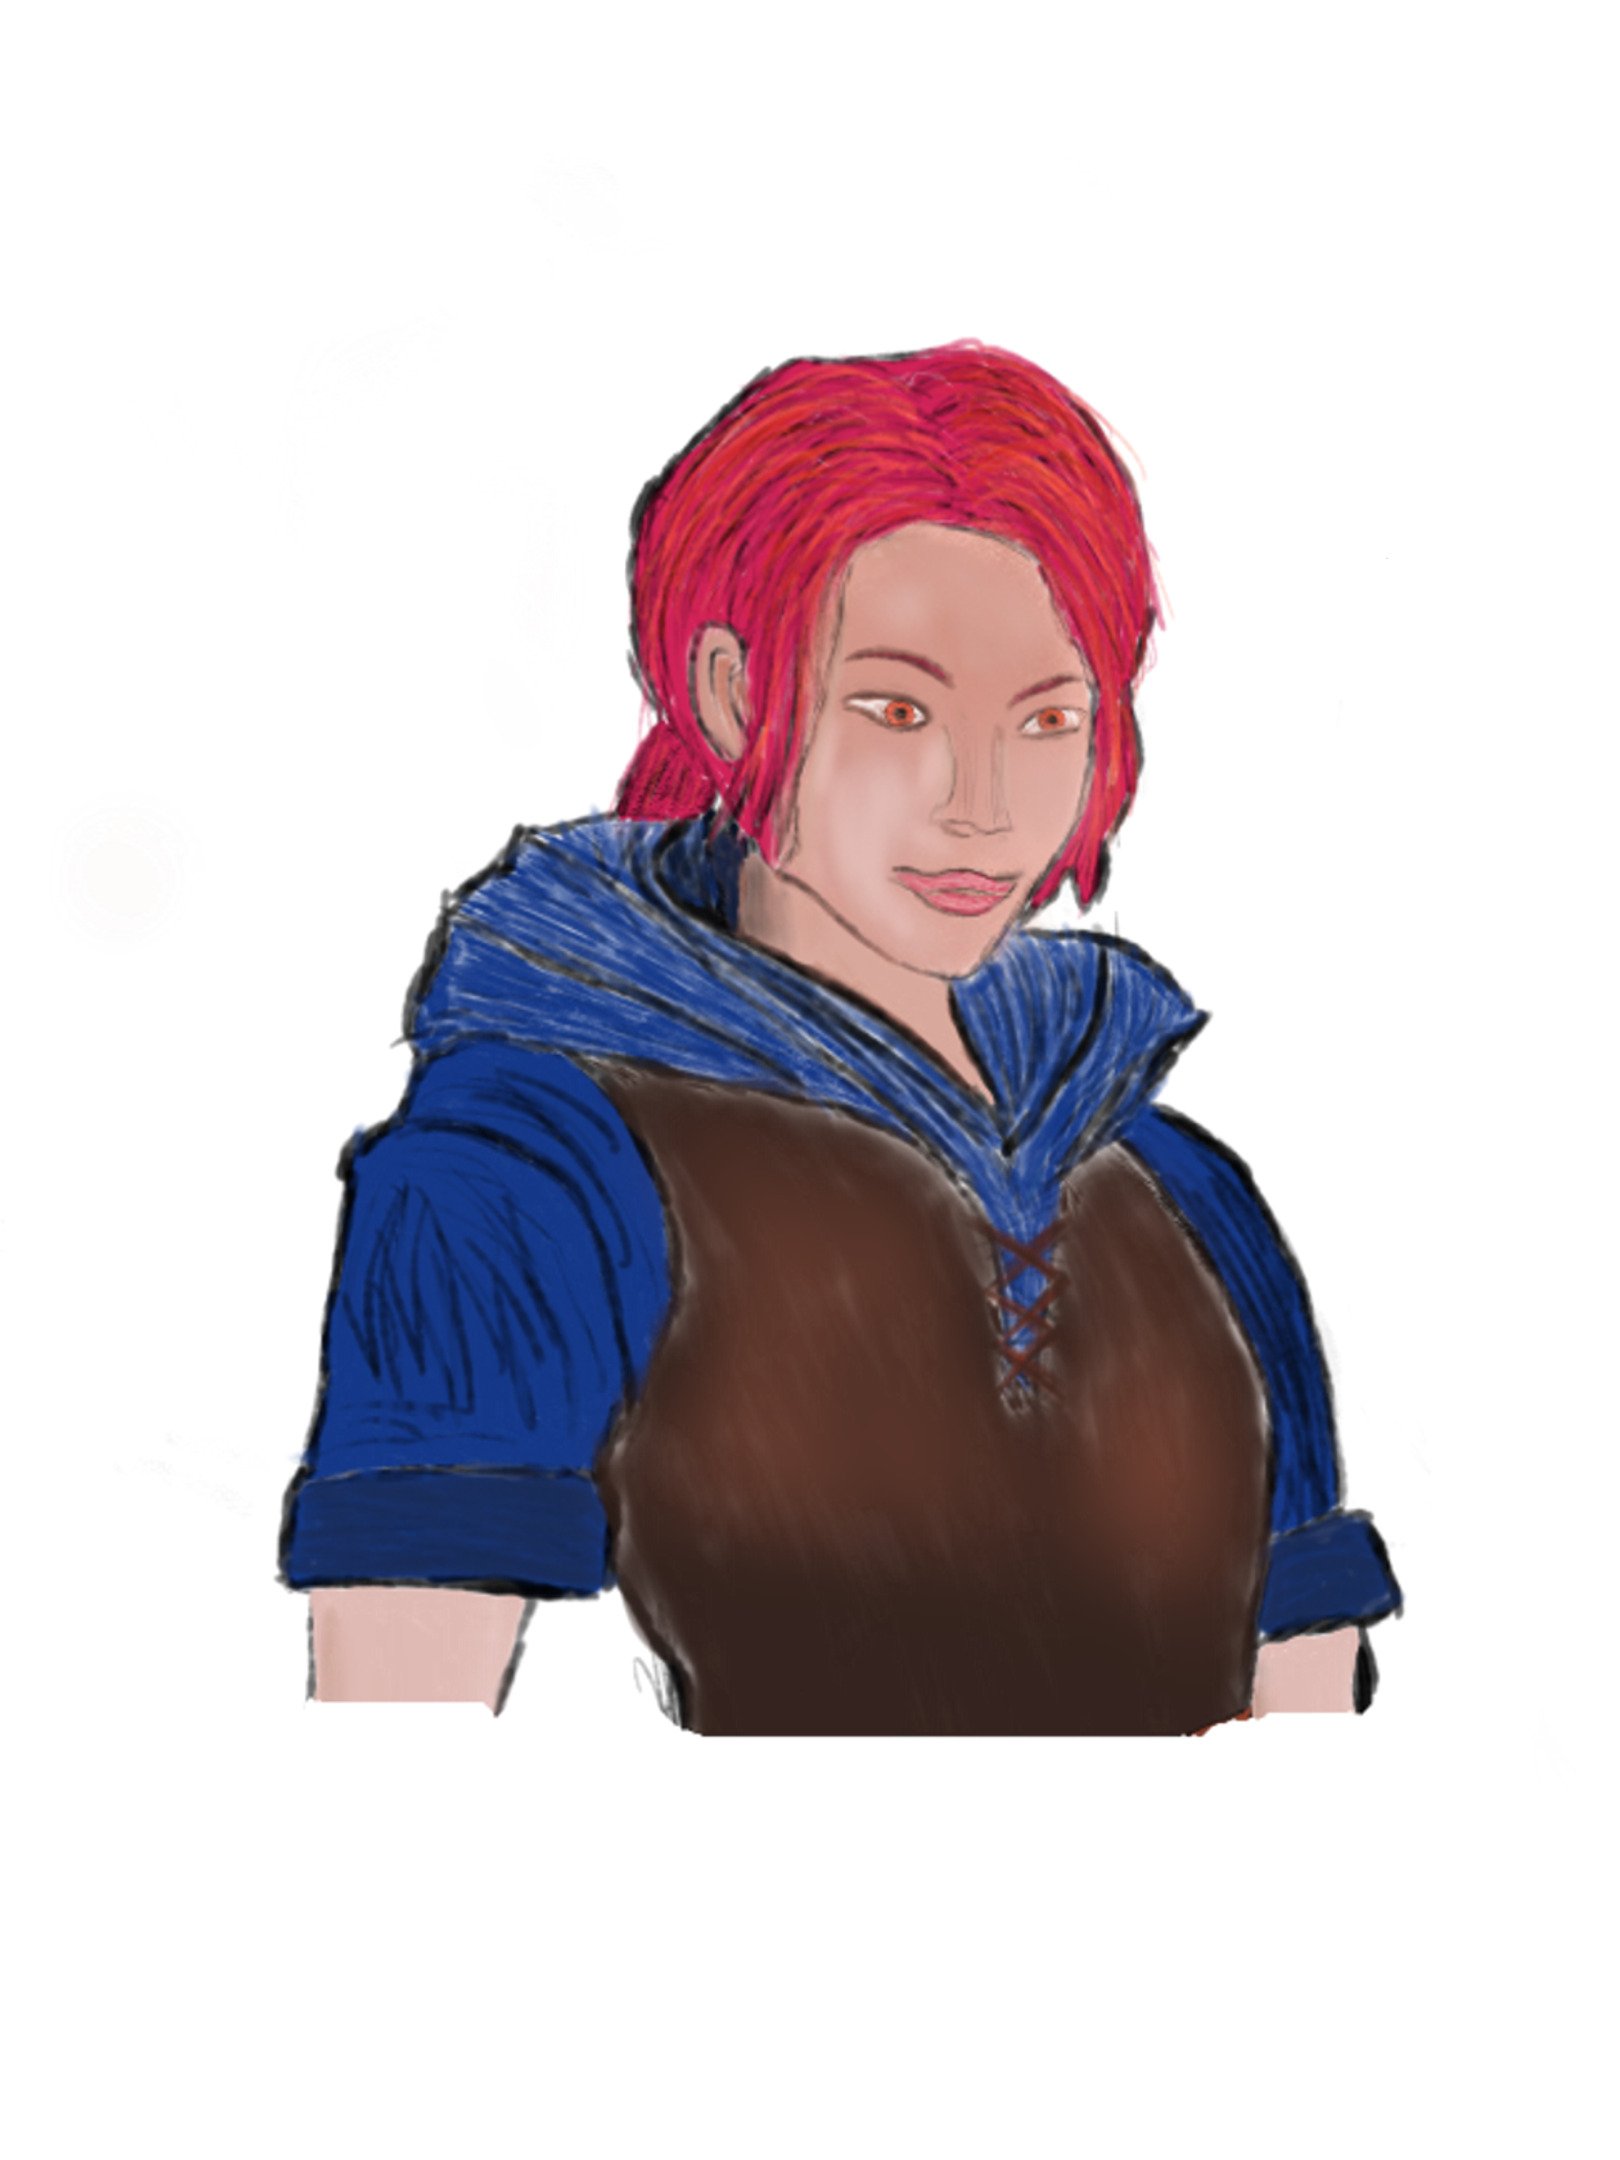
\includegraphics[width=7cm]{Pictures/mensch.png}
		        %\caption{Draekolin}
             \label{fig:Mensch}
        \end{figure}
        

\section*{Artenmerkmale}

\begin{tcolorbox}[title=Artenwerte,colbacktitle=myskin,tabulars={@{\extracolsep{\fill}\hspace{5mm}}cccc@{\hspace{5mm}}},boxrule=0.5pt]
    \textbf{Wunden} & \textbf{Gift} & \textbf{Psyche} & \textbf{Bewegung} \\\hline
    42 & 10 & 10 & 5 \\ \hlineB{3}
    \multicolumn{2}{ r| }{\textbf{Rasse:}} & \multicolumn{2}{ c }{Mischling} \\
    \multicolumn{2}{ r| }{\textbf{Größe:}} & \multicolumn{2}{ c }{Mittel, 1.55 - 1.85 m} \\
    \multicolumn{2}{ r| }{\textbf{Gewicht:}} & \multicolumn{2}{ c }{ 50 - 90 kg} 
\end{tcolorbox}

\subsection*{Genetik der Menschen}
\vspace*{0.75 cm}

\begin{tcolorbox}[title= Herz Genetik,colbacktitle=red, tabulars={@{\extracolsep{\fill}\hspace{5mm}}lc@{\hspace{1mm}}}, boxrule=0.5pt]
    \textbf{Rang 1:} & +2 auf Initiative \\
    \textbf{Rang 2:} & +2 auf Charisma\\
    \textbf{Rang 3:} & +3 auf Psychemaxium\\
    \textbf{Rang 4:} & +2 auf Willenskraft\\
    \textbf{Rang 5:} & Aktion \verweis{sk:wachendes_auge}\\
\end{tcolorbox}
\vspace*{0.4 cm}

\begin{tcolorbox}[title= Pik Genetik,colbacktitle=gray, tabulars={@{\extracolsep{\fill}\hspace{5mm}}lc@{\hspace{1mm}}}, boxrule=0.5pt]
    \textbf{Rang 1:} & +1 auf Robustheit \\
    \textbf{Rang 2:} & +2 auf Kraft \\
    \textbf{Rang 3:} & +7 auf Wundenmaximum \\
    \textbf{Rang 4:} & +1 auf Bewegung \\
    \textbf{Rang 5:} & +5 auf Initiative \\
\end{tcolorbox}
\vspace*{0.4 cm}

\begin{tcolorbox}[title= Karo Genetik,colbacktitle=red, tabulars={@{\extracolsep{\fill}\hspace{5mm}}lc@{\hspace{1mm}}}, boxrule=0.5pt]
    \textbf{Rang 1:} & +2 auf Intelligenz \\
    \textbf{Rang 2:} & +2 auf Giftmaximum \\
    \textbf{Rang 3:} & +3 auf Spirit \\
    \textbf{Rang 4:} & +1 im Element Tod \\
    \textbf{Rang 5:} & Aktion \verweis{sk:lebensraub} \\
\end{tcolorbox}
\vspace*{0.4 cm}

\begin{tcolorbox}[title= Kreuz Genetik, colbacktitle=gray, tabulars={@{\extracolsep{\fill}\hspace{5mm}}lc@{\hspace{1mm}}}, boxrule=0.5pt]
    \textbf{Rang 1:} & Aktion \verweis{sk:freiheitsruf} \\
    \textbf{Rang 2:} & +2 auf Geschicklichkeit \\
    \textbf{Rang 3:} & +2 auf Kreativität\\
    \textbf{Rang 4:} & +2 auf Gifte (benutzten) \\
    \textbf{Rang 5:} & +1 auf Bewegung \\
\end{tcolorbox}

\subsection*{Grundzüge}
Eine der wichtigsten Eigenschaften der Menschen ist ihre Möglichkeit ihr Vertrauen zum Überleben anderen abzugeben und gemeinsam ein Ziel anzugehen, bei dem jeder einzelne für sich nutzlos wäre. Die so mit der Zeit entwickelten Fähigkeiten und Taktiken haben den Menschen bis heute zusammen mit seiner hervorragenden Entwicklungs- und Handarbeit vor dem Aussterben beschützen können. \\
Dein Charakter verfügt von beginn an über die Aktionen: und \verweis{sk:taktieren}, sowie über die Passive: \verweis{sk:Koordinator} 

\subsection*{Koordinator} \label{sk:Koordinator}
Mit schnellen, präzisen Angriffen kann selbst ein übermächtiger Feind in die Knie gezwungen werden.\\
\textbf{Effekt:} \textit{Passiv}. Du darfst in deiner Aktionsphase zwei Karten ablegen, um ein Ziel in 6 m zu nennen. Jede befreundete Kreatur in Reichweite zur gewählten Kreatur (du auch) darf eine Schlagen (Werfen oder Schießen) Probe durchführen.

\subsection*{Taktieren} \label{sk:taktieren}
Mit seinen vorsichtigen Vorgehensweisen ist der Mensch häufig zurückhaltend und schätzt sein Leben über dem Tod seines Feindes.\\
\textbf{Grundwert:} Intelligenz \\
\textbf{Kenntnisschwelle:} 4 \\
\textbf{Anforderung:} Stationär 15+ \\
\textbf{Effekt:} Befreundete Kreaturen im 10 m Radius haben die nächsten \textbf{FK} Aktionsphasen kostenlos Verketten bei ihren Aktionen.

\begin{table}[h!]
    \centering
    \begin{tabular}{|>{\columncolor[RGB]{247, 216, 212}}l|}
    \btrule{1pt}
    \arrayrulecolor{black}
    \\
    \textbf{\large Mensch}\\
    \\
        \begin{tabular}{c|c|c}
           \rowcolor{myred} \begin{tabular}{c}
               \rowcolor{myred}\textbf{Gefahren-}  \\
                \rowcolor{myred} \textbf{wert}\\ 
            \end{tabular} & \textbf{Fähingkeiten} & \textbf{Ausprägung}\\
            \hline
            \rowcolor{myred} 1. & -- & Beruf \\
            \rowcolor{myskin} 2. & 1x Simpel &  Beruf \\
            \rowcolor{myred} 3. & 1x Erweiter & Beruf\\
            \rowcolor{myskin} 4. & 1x Komplex &  Charakterentw. \\
            \rowcolor{myred} 5. & (Spezifisch) &  Beruf\\
            \rowcolor{myskin} 6. & -- & Körperentw. \\
            \rowcolor{myred} 7. & 2x Simpel &  Beruf \\
            \rowcolor{myskin} 8. & 1x Erweitert & Ausbildung\\
            \rowcolor{myred} 9. & 1x Komplex & Beruf\\
            \rowcolor{myskin} 10. & (Spezifisch) & (Spezifisch) \\
            \rowcolor{myred} 11. & -- & Charakterentw.\\
            \rowcolor{myskin} 12. & 1x Simpel & Beruf\\
            \rowcolor{myred} 13. & 2x Erweitert & Körperentw.\\
            \rowcolor{myskin} 14. & 1x Komplex & Ausbildung\\
            \rowcolor{myred} 15. & (Spezifisch) & Beruf\\
            \rowcolor{myskin} 16. & -- & Charakterentw.\\
            \rowcolor{myred} 17. & 1x Simpel & Körperentw.\\
            \rowcolor{myskin} 18. & 1x Erweitert & Beruf \\
            \rowcolor{myred} 19. & 2x Komplex & Ausbildung\\
            \rowcolor{myskin} 20. & (Spezifisch) & Charakterentw.\\
            \rowcolor{myred} 21. & -- & Körperentw.\\
            \rowcolor{myskin} 22. & 2x Simpel & Beruf\\
            \rowcolor{myred} 23. & 2x Erweitert & Charakterentw.\\
            \rowcolor{myskin} 24. & 2x Komplex & Körperentw.\\
            \rowcolor{myred} 25. & (Spezifisch) & Ausbildung \\
            %\rowcolor{myblue} 26. & -- & Pfad\\
            %\rowcolor{myred} 27. & 2x Simpel & \\
            %\rowcolor{myblue} 28. & 2x Erweitert& \\
            %\rowcolor{myred} 29. & 2x Komplex & \\
            %\rowcolor{myblue} 30. &  (Spezifisch) & Pfad\\
        \end{tabular}\\
        \rowcolor{myred}\\
        \btrule{1pt}
    \end{tabular}
\end{table}

\section*{Die Berufungen und Ausbildungen}
Die Fähigkeiten die ein Mensch erlernen kann, hängen nicht nur davon ab zu welchem Berufzweig sie zählen, sondern auch von ihrem Ausbilungsgrad.
Jeder Beruf hat auch eine passende Ausbildung, dies heißt jedoch nicht das man die gleiche Ausbildung wie den Beruf wählen muss. 
Die Ausbildungen haben vier Unterstufen: Anwerter, Novize, Geselle und Meister.

Mit jeder Ausprägung Ausbildung steigst du ein Rang in einer Ausbildung auf. Man kann auch mehrere Ausbildungen als Anwerter aufnehmen, jedoch ist zu beachten das dann die Ausbildung nicht vollendet werden kann.

\subsection*{Schattengestallt $\Herz{}$}
In den dunklen Gossen der Städte lungern die niederen Gestallten der Zivilistationen. Die Schattengestallten haben Zugang zu ruchlosen Mordwerkzeugen, mysteriösen Geheimnissen und unauffälligen Schleichhandlungen. \\
\textbf{Boni:} + 2 Sinne \\
\textbf{Anfangsausrüstung:} Du darfst dir eine Anfangsausrüstung entsprechend eines EWs von Sinne*20 auswählen und erhälst \textit{einfache Kleidung}.\\
\textbf{Startfähigkeit:} \verweis{sk:geisterbund} \\

\subsubsection*{Geisterbund} \label{sk:geisterbund}
Als Gestalt der Schatten hast du ab und zu Kontakt zu Geistern. Auf unergründliche Weise fühlst du dich mit ihnen mehr verbunden, als mit anderen Menschen.
\textbf{Effek:} Du kannst Geister sehen und dich mental mit ihnen unterhalten. Falls dich der Tot ersucht, wanderst du nicht in das Reich der Toten, sondern verlässt deinen vergehenden Körper und verweilst als Geist in den heimlichen Landen. Dieser nicht physische Anteil der Lebenden ist weder mit dem normalen Augen sichtbar, noch anders wahrnehmbar. Anders herum kannst auch du nicht mit der physischen Welt interagieren und lediglich die Geister der Lebenden, die Schatten der festen Objekte und Flüsse des Spiritfeldes sehen.  Flüssigkeiten und Gase sind für dich ebenso wenig vorhanden wie Gravitation. Du hast keine Möglichkeit dich gegen physische Angriffe zu wehren außer du nutzt Ausweichen. Jeder Schaden bringt dich sofort endgültig um. Alleine schon fallender Schnee reicht aus um dich zu durchschlagen und sofort umzubringen. Du kannst dich nur mit Spirit Kreaturen und Personen die über passende Fähigkeiten verfügen unterhalten. Du kannst nur noch Aktionen nutzen die dich selber betreffen oder ausschließlich das Spiritfeld nutzen. Du brauchst weder Schlaf, noch Nahrung, kannst nicht brennen oder durch Temperaturen beeinflusst werden.

\subsubsection*{Weitere}
1. dem Tod entrinnen: Bonus bei vielen Wunden.

\subsubsection*{Ausbildung zum Ruchlosen}
Als frischer \textbf{Anwerter} in der Wildnis der Dunkelheit kannst du \textit{\nameref{sk:freundderschatten}} erlernen.\\

\subsubsection*{Freund der Schatten} \label{sk:freundderschatten}
Der Schatten von Gebäuden, Steinen und Bäumen kann einer unauffälligen Kreatur immense Vorteile gegenüber seines Verfolgers bieten. Gerade mit genug Erfahrung ist es für ein Gegner unglaublich schwer einen geschickt Verstekten zu finden.\\
\textbf{Grundwert:} Gewandheit \\
\textbf{Kenntnisschwelle:} 6 \\
\textbf{Anforderung:} 18+\\
\textbf{Effekt:} Du musst dich innerhalb von einem Meter Entfernung von einem Objekt befinden das min. eine Größenortnung größer als du ist. Du tarnst dich und erhälst somit einen Bonus von 8 auf deine Verteidigung. Sobald du Wunden erleidest, eine Aktion außerhalb eines Schatten bzw. im Nahkampf mit einer Kreatur beendest oder selber angreifst, verblasst die Tarnung. Erhalte ein Vorteil.

\subsubsection*{Todesschütze} \label{sk:todesschütze}
Eine ruhige Atmung, ein freies Schussfeld und die Nerven stählender als die Rüstung des Feinds. Mit einer leisen Bewegung lösen sich die Finger und das Projektil macht sich auf den Weg in sein Ziel.\\
\textbf{Effekt:} \textit{Passiv}. Der Waffenbonus deiner Fernkampfangriffe ist verdoppelt solange du ein Vorteil hast.


Mit erreichen des Grades des \textbf{Novizen} erlernst du....\\
Mit erreichen des Grades des \textbf{Gesellen} erlernst du....\\
Mit erreichen des Grades des \textbf{Meisters} erlernst du....\\


\subsection*{Krieger $\Pik{}$}
Der Aggressor der menschlichen stürmt mit dem Ziel seinen Gegner zu besiegen in die Schlacht. Er kämpft mit jeder Taktik die ihn zum Sieg führt und wird alles geben siegreich zu sein. Als Krieger hat der Spieler eine Auswahl an Angriffen, Taktiken und Kombiantationen zur Verfügung um mit einer Menge Schaden seinen Gegner nieder zu reißen. \\
\textbf{Boni:} \\
\textbf{Anfangsausrüstung:} Du darfst dir eine Anfangsausrüstung entsprechend deines Emotionenwertes*20 auswählen.\\
\textbf{Startfähigkeit:} \verweis{sk:laeufer} \\

\subsubsection*{Läufer} \label{sk:laeufer}
Der Krieger ist es gewohnt in seiner Bewegung inne zu halten und trotz seiner Geschwindigkeit schwerer Angriffe gegen seine Feinde auszuteilen.
\textbf{Effekt:} Wenn du dich nur um die Hälfte der max Bewegungsrate bewegst bist du Stationär.\\
\textbf{Steigerung [15]:}  Du hast den Status ST auch wenn du dich bewegt hast.

\subsubsection*{Ausbildung zum Kriegsmeister}
Als frischer \textbf{Anwerter} kann du .. erlernen.\\
Mit erreichen des Grades des \textbf{Novizen} erlernst du....\\
Mit erreichen des Grades des \textbf{Gesellen} erlernst du....\\
Mit erreichen des Grades des \textbf{Meisters} erlernst du....\\


\subsection*{Gelehrter $\Karo{}$}
Als Antrieb des Fortschritts liegt es an den Gelehrten das Wissen in die Heimliche Welt zu tragen, zu forschen und den Niederen unterstützen. Der Gelehrte sammelt Informationen über Gegner, heilt Verbündete und kann Versuchen die hohen Künsten des Manifestationen zu beherschen.\\
\textbf{Boni:} \\
\textbf{Anfangsausrüstung:} Du darfst dir eine Anfangsausrüstung entsprechend deines Intelligenzwertes*25 auswählen.\\
\textbf{Startfähigkeit:} \verweis{sk:Vertrauen_in_das_höhere_Wohl} \\

\subsubsection*{Vertrauen in das höhere Wohl} \label{sk:Vertrauen_in_das_höhere_Wohl}
Das Vertrauen in einen größeren Sinn hat den Menschen schon zu vielen großartigen Handlungen angetrieben. Mit diesem Gedankenkonzept im Hinterkopf traut sich der Philosoph viel mehr zu als was man von ihm erwartet hätte. \\
\textbf{Effekt:} Du darfst in deiner Ausweichen-Aktion statt Gewandtheit deinen Spiritwert nutzen.\\
\textbf{Steigerung [15]:} Du darfst auch in deiner Blocken-Aktion deinen Spiritwert nutzen.

\subsubsection*{Mysteriöse Kriegsführung} \label{sk:Mysteriöse Kriegsführung}
............................ \\
\textbf{Effekt:} Du darfst für deine Schlagen-Aktion deinen Spiritwert nutzen.\\

\subsubsection*{Ausbildung zum Wissenshüter}
Der angehende \textbf{Anwerter} hat Zugang zu \textit{\nameref{sk:beobachten}}.\\
Als \textbf{Novize} des Wissens stehen dir neue Tore offen. So kannst du \textit{\nameref{sk:wissenistmacht}}, \verweis{sk:inspirierend} erlernen.\\

\subsubsection*{Inspirierend} \label{sk:inspirierend}
Allein deine Präsenz lässt Mensch und Kreatur zu großem fähig werden.
\textbf{Effekt:} Du darfst jede Kampfrunde einmal den Mindestwert einer Aktion einer befreundeten Kreatur in Sichtfeld um 3 senken.\\
\textbf{Steigerung [15]:} Der Wert steigt auf 5 und kann zweimal genutzt werden.\\
\textbf{Steigerung [25]:} Kann 5 mal pro Kampfrunde genutzt werden.

Mit erreichen des Grades des \textbf{Gesellen} erlernst du....\\


Mit erreichen des Grades des \textbf{Meisters} erlernst du....\\


\subsection*{Arbeiter $\Kreuz{}$}
Der fleißige Arbeiter ist der Schöpfer von neuen Werke und ist die stütze der Menschheit. Er schwitzt und schafft, werkelt und macht weiter. Als Arbeiter erhälst du Zugang zu Fähigkeiten Gegenstände zu erschaffen, Waffen und Rüstungen aufzubessern, zu kochen und wie der Pöbel zu denken.\\
\textbf{Boni:} \\
\textbf{Anfangsausrüstung:} Du darfst dir eine Anfangsausrüstung entsprechend deines Charima*20 auswählen. \\
\textbf{Startfähigkeit:} \verweis{sk:taktisches_gespür} \\

\subsubsection*{Taktisches Gespür} \label{sk:taktisches_gespür}
Mit koordinierten Absprachen und guten Ideen können Kämpfe auf einer ganz anderen Ebene entschieden werden.
\textbf{Effekt:} Du darfst einmal pro Kampf für eine Aktionsphase die Initiativreihenfolge bestimmen.\\
\textbf{Steigerung [15]:} Du kannst den Effekt jetzt zweimal pro Kampf nutzen.

\subsubsection*{Ausbildung zum Berater}
Als motivierter aber unerfahrener \textbf{Anwerter} des Handwerks stehen dir folgende Fähigkeiten zur Verfügung:.\\
Als \textbf{Novize}  kannst du ... erlernen.\\
Mit erreichen des Grades des \textbf{Gesellen} erlernst du....\\
Mit erreichen des Grades des \textbf{Meisters} erlernst du....\\

\subsection*{Menschennamen:}

\subsubsection*{weiblich:}
Larissa Meinla

% = = = = = = = = = = = = = = = = %
\clearpage

\section{Mrots} \label{art:mrots}

\begin{figure}[htbp]
		        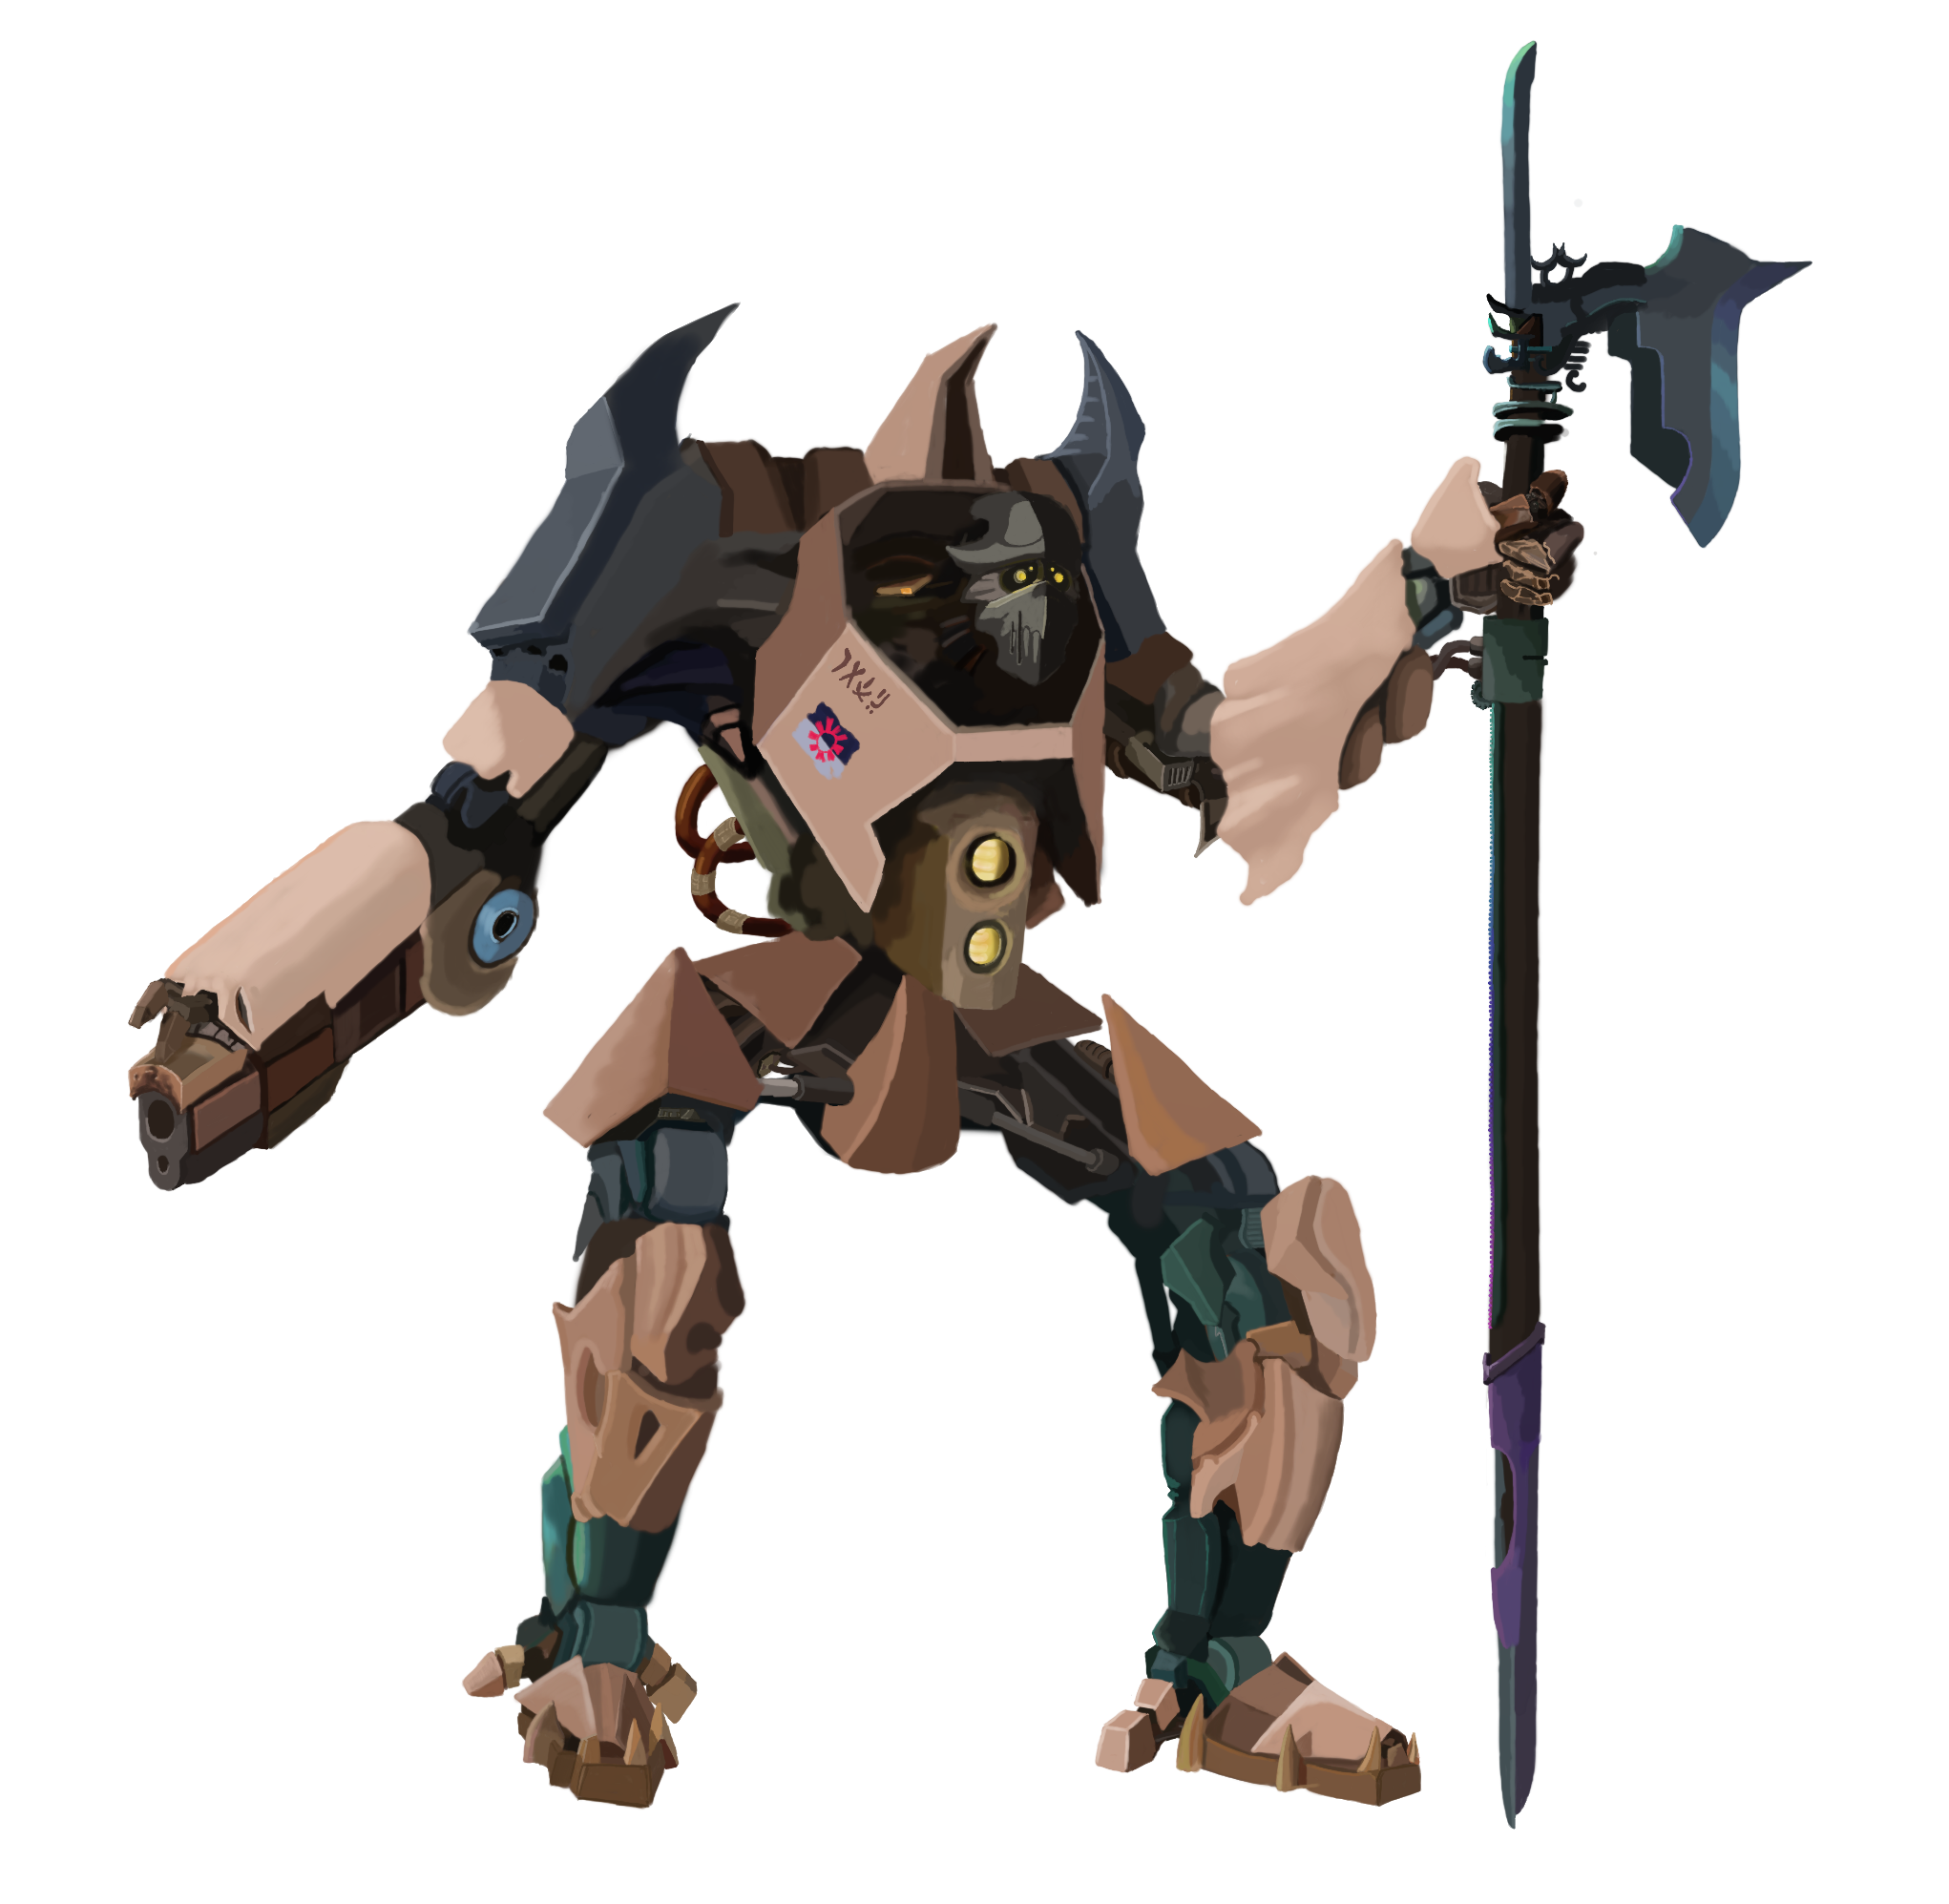
\includegraphics[width=8cm]{Pictures/Mrot.png}
		        %\caption{Mrot}
             \label{fig:Mrot}
        \end{figure}

Als Mrots wird jede Laufende Maschine der Orks bezeichnet. Sei es ein zweibeiniger Arbeiter, ein vierbeiniges Katzenroboter oder eine mächtiger Kampfläufer. Sie lassen sich leicht an Situationen anpassen, können Arbeiten übernehmen zu denen niemand anderes fähig wäre und sind für ihre humorlose Art bekannt.

\section*{Artenmerkmale}

\begin{tcolorbox}[title=Artenwerte,colbacktitle=mysilver,tabulars={@{\extracolsep{\fill}\hspace{5mm}}cccc@{\hspace{5mm}}},boxrule=0.5pt]
    \textbf{Wunden} & \textbf{Gift} & \textbf{Psyche} & \textbf{Bewegung} \\\hline
    38 & 17 & 11 & 5\\ \hlineB{3}
    \multicolumn{2}{ r| }{\textbf{Rasse:}} & \multicolumn{2}{ c }{Mechanismus} \\
    \multicolumn{2}{ r| }{\textbf{Größe:}} & \multicolumn{2}{ c }{Mittel, 1.6 - 1.7 m} \\
    \multicolumn{2}{ r| }{\textbf{Gewicht:}} & \multicolumn{2}{ c }{ 85 - 125 kg} 
\end{tcolorbox}

\subsection*{Schaltkreise der Mrots}
\vspace*{0.75 cm}

\begin{tcolorbox}[title= Herz Schaltkreise,colbacktitle=red, tabulars={@{\extracolsep{\fill}\hspace{5mm}}lc@{\hspace{1mm}}}, boxrule=0.5pt]
    \textbf{Rang 1:} & +2 auf Gewandtheit \\
    \textbf{Rang 2:} & +3 auf Giftmaximum\\
    \textbf{Rang 3:} & +2 auf Kreativität\\
    \textbf{Rang 4:} & +1 auf Ladungsmaximum\\
    \textbf{Rang 5:} & Modul \verweis{entw:infrasicht}\\
\end{tcolorbox}
\vspace*{0.4 cm}

\begin{tcolorbox}[title= Pik Schaltkreise, colbacktitle=gray, tabulars={@{\extracolsep{\fill}\hspace{5mm}}lc@{\hspace{1mm}}}, boxrule=0.5pt]
    \textbf{Rang 1:} & +4 auf Wundenmaximum \\
    \textbf{Rang 2:} & Aktion \verweis{sk:rücksichtsloses_schlagen} \\
    \textbf{Rang 3:} & +2 auf Robustheit \\
    \textbf{Rang 4:} & +1 auf Bewegung \\
    \textbf{Rang 5:} & +3 auf Kraft \\
\end{tcolorbox}
\vspace*{0.4 cm}

\begin{tcolorbox}[title= Karo Schaltkreise, colbacktitle=red, tabulars={@{\extracolsep{\fill}\hspace{5mm}}lc@{\hspace{1mm}}}, boxrule=0.5pt]
    \textbf{Rang 1:} & +1 auf Ladungsmaximum \\
    \textbf{Rang 2:} & +2 auf Spirit \\
    \textbf{Rang 3:} & +2 im Element Sturm  \\
    \textbf{Rang 4:} & +2 auf Energiemaximum  \\
    \textbf{Rang 5:} & +2 auf Psychemaximum \\
\end{tcolorbox}
\vspace*{0.4 cm}

\begin{tcolorbox}[title= Kreuz Schaltkreise, colbacktitle=gray, tabulars={@{\extracolsep{\fill}\hspace{5mm}}lc@{\hspace{1mm}}}, boxrule=0.5pt]
    \textbf{Rang 1:} & +2 auf Geschicklichkeit \\
    \textbf{Rang 2:} & +2 auf Initiative \\
    \textbf{Rang 3:} & Passive \verweis{sk:uebertaktung}\\
    \textbf{Rang 4:} & +2 auf Willenskraft \\
    \textbf{Rang 5:} & +1 auf Modulmaximum \\
\end{tcolorbox}

\subsection*{Grundzüge}
......................... \\
Gifte entfalten wie unter \textit{\nameref{mechanismus}} beschrieben nicht ihre übliche Wirkung. Eine Ausnahme liefern jedoch Mrots die mit dem \verweis{biocore} betrieben werden.
Dein Charakter verfügt von Beginn an über die Aktionen: \verweis{sk:laden}, \verweis{sk:ladungsexplosionsimpulse} und \verweis{sk:ueberladen}, sowie über die Passiven: \verweis{sk:ladungstraeger} und \verweis{sk:ladungswandler}

\subsection*{Laden} \label{sk:laden}
Der Mrot kann seine mechanischen Systeme zurückfahren und so seine Energiespeicher vorspeichern um seine Energie zu einem taktisch besseren Zeitpunkt seine wertvollen Resourcen besser einsetzen zu können.\\
\textbf{Grundwert:} Spirit \\
\textbf{Kenntnisschwelle:} 1 \\
\textbf{Anforderung:} Stationär $\Karo{}$ \\
\textbf{Effekt:} Erhalte bis zu \textbf{FK} Ladungen, kann nicht das Maximum übersteigen.

\subsection*{Ladungsexplosionsimpulse } \label{sk:ladungsexplosionsimpulse}
Mit einer plötzlichen Zellzündung kreiert der Mrot eine mechanischen Unterdruck im Nebenkern und kann Hochenergieimpulse auf seine Gegner loslassen.\\
\textbf{Grundwert:} Spirit \\
\textbf{Kenntnisschwelle:} 3 \\
\textbf{Anforderung:} Stationär 25+ \\
\textbf{Effekt:} \textit{Angriff (Physisch)}. Gebe alle Ladungen aus, um jeder anderen Kreatur im Radius von 3m pro ausgegebener Ladung einen Schaden zuzufügen. \textbf{Bonus:} Element Sturm.

\subsection*{Ladungsträger} \label{sk:ladungstraeger}
Der Mrot besitzt neben seinem Primärenergiespeicher Nebenzellen um überschüssige Energie zu speichern.
\textbf{Effekt:} \textit{Passiv.}Du kannst bis zu 2 Ladungen speichern. Ladungen ermöglichen es dir gewisse Aktionen zu verwenden oder Bonuseffekte bei Aktionen zu erhalten.

\subsection*{Ladungswandler} \label{sk:ladungswandler}
Gespeicherte Energien können genutzt werden um Energie intensive Prozesse zu unterstützen.\\
\textbf{Effekt:} \textit{Passiv.}Du kannst eine Ladung ausgeben um dein Element Sturm zu der Aktion zu addierten die du gerade ausführst. Die Aktion muss Physischer oder Elementarer Natur sein. Wenn immer du das Leiden \verweis{ef:geschockt} erhältst generiere eine Ladung.

\subsection*{Überladen} \label{sk:ueberladen}
Über das Ladungsprotokoll können die Hauptzündungsleistungen überlastet werden um kurzzeitig zusätzliche Energien freizusetzen.\\
\textbf{Grundwert:} Spirit \\
\textbf{Kenntnisschwelle:} 2 \\
\textbf{Anforderung:} 15+ \\
\textbf{Reichweite:} 0.5 m\\
\textbf{Effekt:} \textit{Angriff (Physisch)}.Gebe bis zu \textbf{FK} Ladungen aus, um das Ziel pro ausgegebener Ladung eine Aktionsphase lang zu schocken. \textbf{Bonus:} Element Sturm.
\subsubsection*{Technischer Fortschritt}
Mrots entwickeln sich im Gegensatz zu anderen Arten nicht im biologischen Sinne weiter. Dafür aber können sie nach und nach ihre Bestandteile austauschen und aufwerten. Um Teile auszutauschen benötigt es eine \textbf{mittler Probe (16+)} auf Geschicklichkeit. Zu dem benötigt es Hände um Teile aus und ein zu bauen. Eine ausführliche Liste aller Teile finden sich im Kapitel \textit{\nameref{ent:mrots}}.

\begin{table}[h!]
    \centering
    \begin{tabular}{|>{\columncolor[RGB]{247, 216, 212}}l|}
    \btrule{1pt}
    \arrayrulecolor{black}
    \\
    \textbf{\large Mrots}\\
    \\
        \begin{tabular}{c|c|c}
           \rowcolor{myred} \begin{tabular}{c}
               \rowcolor{myred}\textbf{Gefahren-}  \\
                \rowcolor{myred} \textbf{wert}\\ 
            \end{tabular} & \textbf{Fähingkeiten} & \textbf{Ausprägung}\\
            \hline
            \rowcolor{myred} 1. & -- & Kern \\
            \rowcolor{mysilver} 2. & 1x Simpel &  Kern \\
            \rowcolor{myred} 3. & 1x Erweiter & Kern\\
            \rowcolor{mysilver} 4. & 1x Komplex &  Körperentw. \\
            \rowcolor{myred} 5. & (Spezifisch) &  Kern\\
            \rowcolor{mysilver} 6. & -- & Charakterentw.. \\
            \rowcolor{myred} 7. & 2x Simpel &  Kern \\
            \rowcolor{mysilver} 8. & 1x Erweitert & (Spezifisch)\\
            \rowcolor{myred} 9. & 1x Komplex & Kern\\
            \rowcolor{mysilver} 10. & (Spezifisch) & (Spezifisch) \\
            \rowcolor{myred} 11. & -- & Körperentw.\\
            \rowcolor{mysilver} 12. & 1x Simpel & Kern\\
            \rowcolor{myred} 13. & 2x Erweitert & Charakterentw..\\
            \rowcolor{mysilver} 14. & 1x Komplex & (Spezifisch)\\
            \rowcolor{myred} 15. & (Spezifisch) & Kern\\
            \rowcolor{mysilver} 16. & -- & Körperentw.\\
            \rowcolor{myred} 17. & 1x Simpel & Charakterentw..\\
            \rowcolor{mysilver} 18. & 1x Erweitert & Kern \\
            \rowcolor{myred} 19. & 2x Komplex & (Spezifisch)\\
            \rowcolor{mysilver} 20. & (Spezifisch) & Körperentw.\\
            \rowcolor{myred} 21. & -- & Charakterentw..\\
            \rowcolor{mysilver} 22. & 2x Simpel & Kern\\
            \rowcolor{myred} 23. & 2x Erweitert & Körperentw.\\
            \rowcolor{mysilver} 24. & 2x Komplex & Charakterentw..\\
            \rowcolor{myred} 25. & (Spezifisch) & (Spezifisch) \\
            %\rowcolor{myblue} 26. & -- & Pfad\\
            %\rowcolor{myred} 27. & 2x Simpel & \\
            %\rowcolor{myblue} 28. & 2x Erweitert& \\
            %\rowcolor{myred} 29. & 2x Komplex & \\
            %\rowcolor{myblue} 30. &  (Spezifisch) & Pfad\\
        \end{tabular}\\
        \rowcolor{myred}\\
        \btrule{1pt}
    \end{tabular}
\end{table}


\section*{Die erste Kernzündung}
Das Zusammenbauen eines Mrots ist ein einzigartiges Baukastengefühl. Bevor du jedoch anfängst den Lötzinn raus zu kramen braucht es erst einmal deinen Energie-Core. Die Cores stellen die Energiequelle der Mrots da und verkörpern ihren Geist. Auch wenn sie allesamt einzigartige Wunder aus Orkhänden sind, können sie in Kategorien unterteilt werden. Ein Core darf um 5 zusätzliche Energieeinheiten zu liefern übersteuert werden. Da die Hauptbestandteile darunter jedoch leiden, werden für die Dauer der Übersteuerung alle Körperattribute um eins gesenkt.

\subsection*{Heavycore $\Herz{}$}
Der Heavycore ist ein absolutes Energiebiest. Mit einer einzigartigen Energierate kann er ohne Probleme Superheavy-Kampfsysteme mit Energieversorgen ohne übersteuert werden zu müssen.\\
\textbf{Energiebeitrag:} 17 \\
\textbf{Boni:} \\
\textbf{Anfangsausrüstung:} MK-I Powerbox als Strucktur und Module im Wert von 2000 EW \\

\subsection*{Warcore $\Pik{}$}
Der Warcore wird für besonders schwere Lastarbeiter und schwere Kriegermorts verwendet.\\
\textbf{Energiebeitrag:} 15 \\
\textbf{Boni:} +2 Kraft \& +2 Robustheit \\
\textbf{Anfangsausrüstung:} MK-I Powerbox als Strucktur und Module im Wert von 2000 EW\\

\subsection*{Spiritcore $\Karo{}$}
Über ein besonderes Schwingungsmodul entwickelte die Orkentwicklungsgruppe Ewida diesen besonders feinen spiritnahen freischwingenden Maincore. Diese Freiheit ermöglicht es dem Mrot einfacher Energie zu manesfestieren und so mit mehr Blitze auf seine Opferregnen zu lassen.\\
\textbf{Energiebeitrag:} 12 \\
\textbf{Boni:} +2 Spirit \& +2 Element Sturm \\
\textbf{Anfangsausrüstung:} MK-I Powerbox als Strucktur und Module im Wert von 2000 EW \\

\subsection*{Biocore $\Kreuz{}$} \label{biocore}
Der Biocore wurde entwickelt um Mrots zu schaffen die den lebenden Kreaturen ähneln. \\
\textbf{Energiebeitrag:} 13 \\
\textbf{Boni:} Du kannst Essen und Trinken so wie andere Lebewesen und deine Energie aus der Nahrung beziehen. Desweitern kannst du aus Biomasse Ladungen generieren. \\
\textbf{Anfangsausrüstung:} MK-I Powerbox als Strucktur und Module im Wert von 2000 EW \\
\textbf{Startfertigkeit:}\verweis{sk:ladungsverzer}

\subsubsection*{Ladungsverzehr} \label{sk:ladungsverzer}
Es ist dir möglich Ladungen auch biologisch zu verarbeiten. Durch das biologische Verarbeiten von Ladungen erhältst du einen Metabolismus schub.\\
\textbf{Effekt:} Du kannst eine Ladung verbrauchen um deine Gewandtheit und Bewegung zu verdoppeln. Dies muss am Anfang deiner Aktionsphase angesagt werden und endet mit deiner nächsten Aktionsphase (auch wenn du keine Aktion ausführen kannst).


% = = = = = = = = = = = = = = = = %
\clearpage

\section{Skriva} \label{art:skriva}

\begin{figure}[htbp]
		        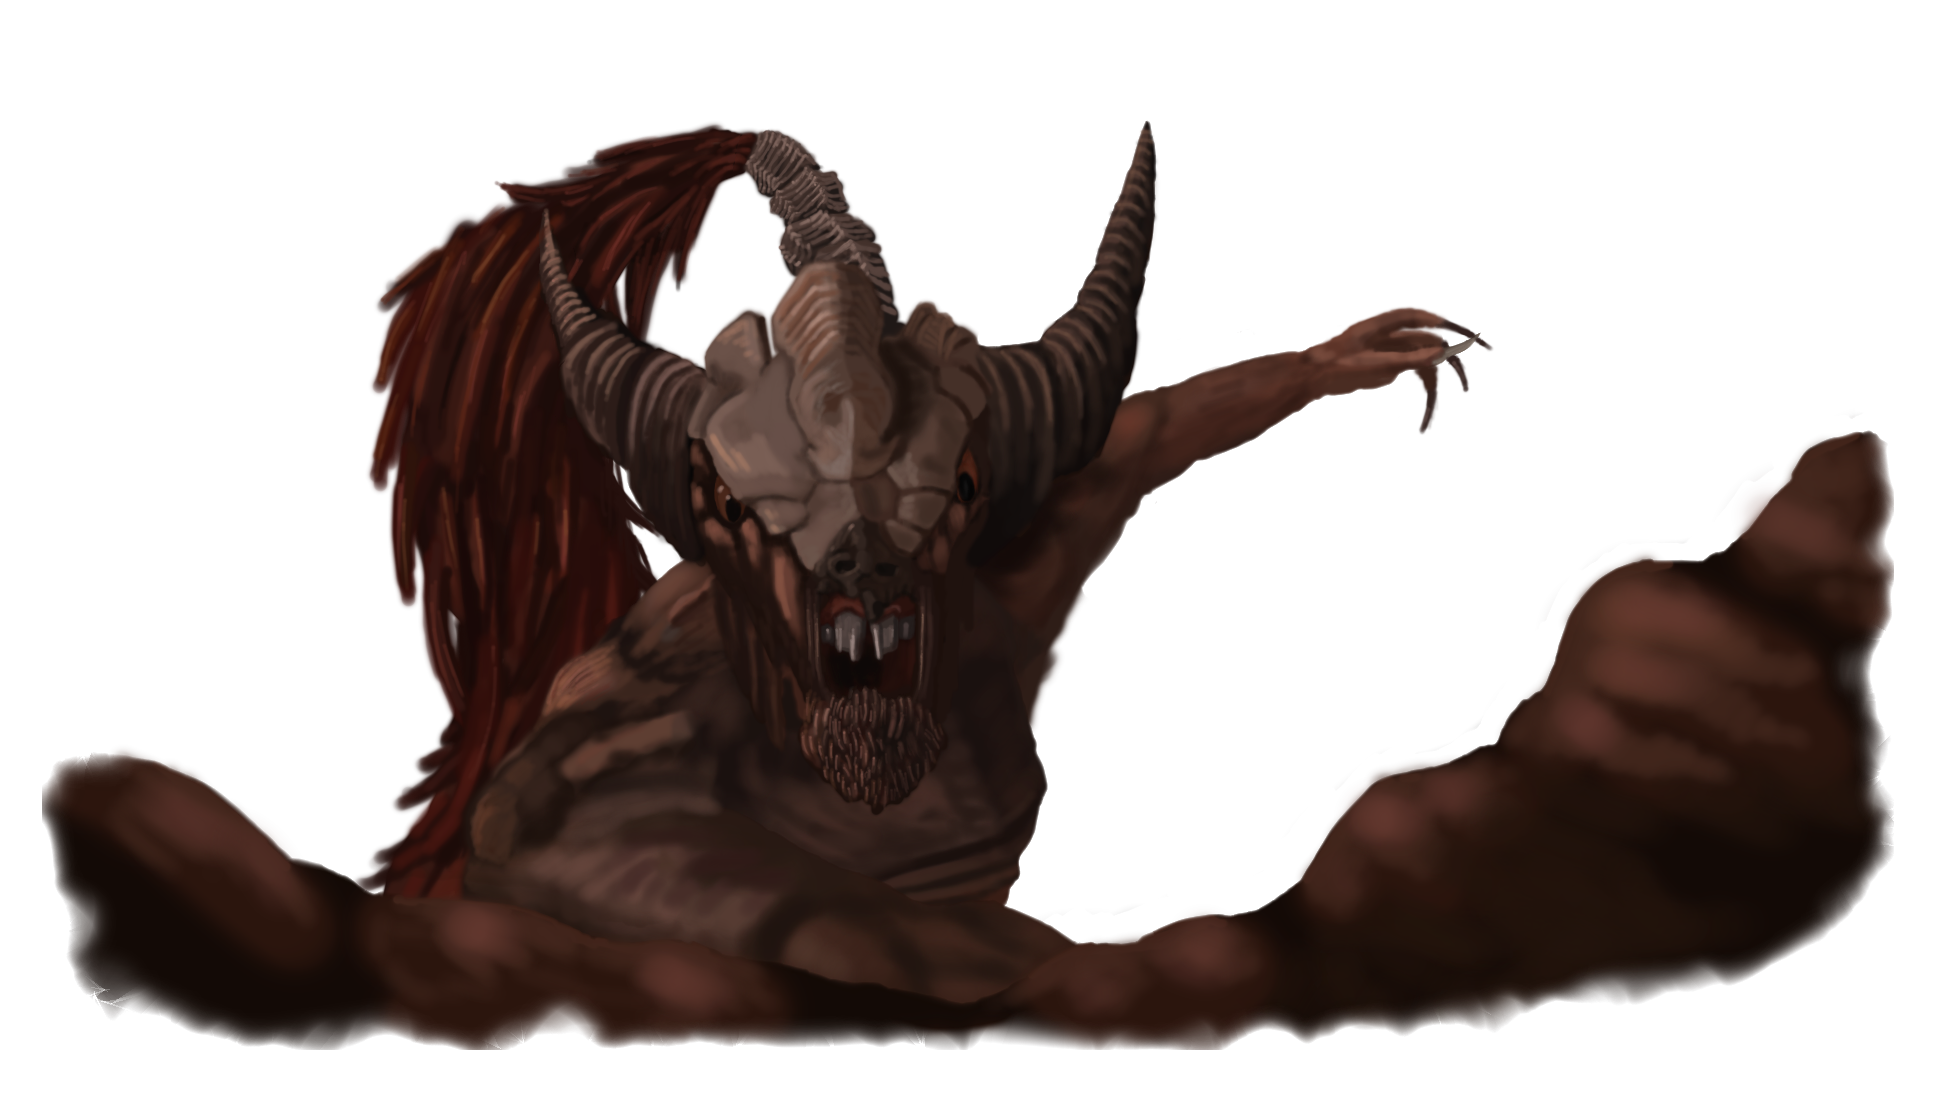
\includegraphics[width=8cm]{Pictures/Razzorrat.png}
		        %\caption{Skriva}
             \label{fig:Skriva}
        \end{figure}
        
Im Gegensatz zu vielen anderen Arten konzentrieren sich die Skirva nicht darauf besonders viele Dinge zu erlernen, sondern darauf ihre eigenen Fähigkeiten optimal zu nutzen. 

\section*{Artenmerkmale}

\begin{tcolorbox}[title=Artenwerte,colbacktitle=mygreen,tabulars={@{\extracolsep{\fill}\hspace{5mm}}cccc@{\hspace{5mm}}},boxrule=0.5pt]
    \textbf{Wunden} & \textbf{Gift} & \textbf{Psyche} & \textbf{Bewegung} \\\hline
    37 & 14 & 9 & 5 \\ \hlineB{3}
    \multicolumn{2}{ r }{\textbf{Rasse:}} & \multicolumn{2}{ c }{Kratzer} \\
    \multicolumn{2}{ r }{\textbf{Größe:}} & \multicolumn{2}{ c }{Mittel} \\
    \multicolumn{2}{ r }{\textbf{Gewicht:}} & \multicolumn{2}{ c }{Mittel} 
\end{tcolorbox}

\subsection*{Genetik der Skriva}
\vspace*{0.75 cm}

\begin{tcolorbox}[title= Herz Genetik, colbacktitle=red, tabulars={@{\extracolsep{\fill}\hspace{5mm}}lc@{\hspace{1mm}}}, boxrule=0.5pt]
    \textbf{Rang 1:} & +2 auf Toxin \\
    \textbf{Rang 2:} & Aktion \verweis{sk:furie} \\
    \textbf{Rang 3:} & +2 auf Gewandtheit  \\
    \textbf{Rang 4:} & +2 auf Geschicklichkeit  \\
    \textbf{Rang 5:} & Aktion \verweis{sk:eingraben} \\
\end{tcolorbox}
\vspace*{0.4 cm}

\begin{tcolorbox}[title= Pik Genetik, colbacktitle=gray, tabulars={@{\extracolsep{\fill}\hspace{5mm}}lc@{\hspace{1mm}}}, boxrule=0.5pt]
    \textbf{Rang 1:} & +2 Robustheit \\
    \textbf{Rang 2:} & +5 auf Wundenmaximum \\
    \textbf{Rang 3:} & Passive \verweis{sk:starkes_gewebe} \\
    \textbf{Rang 4:} & +3 auf Kreativität \\
    \textbf{Rang 5:} & +2 auf Kraft \\
\end{tcolorbox}
\vspace*{0.4 cm}

\begin{tcolorbox}[title= Karo Genetik, colbacktitle=red, tabulars={@{\extracolsep{\fill}\hspace{5mm}}lc@{\hspace{1mm}}}, boxrule=0.5pt]
    \textbf{Rang 1:} & +2 auf Geschicklichkeit \\
    \textbf{Rang 2:} & +2 auf Willenskraft \\
    \textbf{Rang 3:} & +2 auf Spirit \\
    \textbf{Rang 4:} & Aktion \verweis{sk:totstellen}\\
    \textbf{Rang 5:} & +4 auf Toxin \\
\end{tcolorbox}
\vspace*{0.4 cm}

\begin{tcolorbox}[title= Kreuz Genetik,colbacktitle=gray, tabulars={@{\extracolsep{\fill}\hspace{5mm}}lc@{\hspace{1mm}}}, boxrule=0.5pt]
    \textbf{Rang 1:} & +2 auf Giftmaximum \\
    \textbf{Rang 2:} & +2 auf Toxin \\
    \textbf{Rang 3:} & +2 auf Wundenmaximum \\
    \textbf{Rang 4:} & +2 auf Initiative \\
    \textbf{Rang 5:} & +4 auf Psychemaximum \\
\end{tcolorbox}

\subsection*{Grundzüge}
Ihr Leben in der Kanalisation hat die Skriva den Umgang mit Gift gelehrt.
Skriva beginnen ihre Reise mit dem Merkmal \textit{\nameref{ef:toxin} 1} und einem \textit{schwächenden Gift}.\\
Dein Charakter verfügt von beginn an über die Aktionen: \verweis{sk:toxinstich} und \verweis{sk:saeurespeien} , sowie die Passive: \verweis{sk:volk_der_unterwelt}.

\subsection*{Säurespeien} \label{sk:saeurespeien}
Als wahrer Allesfresser benötigen die Skriva besondere Säuren um mit den Fremdkörpern klar zu kommen. Wenn diese Säuren jedoch ausgespuckt werden sind sie umso schrecklicher.\\
\textbf{Grundwert:} Geschicklichkeit \\
\textbf{Kenntnisschwelle:} 3 \\
\textbf{Maximale Kenntnis:} 8 \\
\textbf{Anforderung:} 18+ \\
\textbf{Effekt:} \textit{Angriff (Gift)}. Reduziere die Rüstung des Ziels um \textbf{FK}. \textbf{Bonus:} Toxin.

\subsection*{Toxinstich} \label{sk:toxinstich}
Mit einer flinken Bewegung sticht der wendige Skriva seinen Klauenbesetzen Schwanz in die Organe seines Gegners. Das übertragende Gift kann nun frei im langsam zerfallenden Körper propagieren.\\
\textbf{Grundwert:} Geschicklichkeit \\
\textbf{Kenntnisschwelle:} 2 \\
\textbf{Maximale Kenntnis:} 20 \\
\textbf{Anforderung:} Bewegt \\
\textbf{Reichweite:} 0.75 m \\
\textbf{Effekt:} \textit{Angriff (Gift)}. Sollte eine Kreatur Giftwunden erleiden, so erleidet sie den Effekt deines Giftes. \textbf{Bonus:} Toxin.

\subsection*{Volk der Unterwelt} \label{sk:volk_der_unterwelt}
Durch ihr Leben in der dunklen Unterwelt haben die Skriva ihren Sehsinn optimiert.\\
\textbf{Effekt:} \textit{Passive.} Du kannst in Dämmerung auf 50 m noch normal sehen und in Dunkelheit 30 m. Allerdings bist du leicht zu blenden.

\begin{table}[h!]
    \centering
    \begin{tabular}{|>{\columncolor[RGB]{247, 216, 212}}l|}
    \btrule{1pt}
    \arrayrulecolor{black}
    \\
    \textbf{\large Skriva}\\
    \\
        \begin{tabular}{c|c|c}
           \rowcolor{myred} \begin{tabular}{c}
               \rowcolor{myred}\textbf{Gefahren-}  \\
                \rowcolor{myred} \textbf{wert}\\ 
            \end{tabular} & \textbf{Fähingkeiten} & \textbf{Ausprägung}\\
            \hline
            \rowcolor{myred} 1. & -- & Brut \\
            \rowcolor{mygreen} 2. & 1x Simpel &  Brut \\
            \rowcolor{myred} 3. & 1x Erweiter & Brut\\
            \rowcolor{mygreen} 4. & 1x Komplex &  Körperentw. \\
            \rowcolor{myred} 5. & (Spezifisch) &  Brut\\
            \rowcolor{mygreen} 6. & -- & Charakterentw.. \\
            \rowcolor{myred} 7. & 2x Simpel &  Brut \\
            \rowcolor{mygreen} 8. & 1x Erweitert & (Spezifisch)\\
            \rowcolor{myred} 9. & 1x Komplex & Brut\\
            \rowcolor{mygreen} 10. & (Spezifisch) & (Spezifisch) \\
            \rowcolor{myred} 11. & -- & Körperentw.\\
            \rowcolor{mygreen} 12. & 1x Simpel & Brut\\
            \rowcolor{myred} 13. & 2x Erweitert & Charakterentw..\\
            \rowcolor{mygreen} 14. & 1x Komplex & (Spezifisch)\\
            \rowcolor{myred} 15. & (Spezifisch) & Brut\\
            \rowcolor{mygreen} 16. & -- & Körperentw.\\
            \rowcolor{myred} 17. & 1x Simpel & Charakterentw..\\
            \rowcolor{mygreen} 18. & 1x Erweitert & Brut \\
            \rowcolor{myred} 19. & 2x Komplex & (Spezifisch)\\
            \rowcolor{mygreen} 20. & (Spezifisch) & Körperentw.\\
            \rowcolor{myred} 21. & -- & Charakterentw..\\
            \rowcolor{mygreen} 22. & 2x Simpel & Brut\\
            \rowcolor{myred} 23. & 2x Erweitert & Körperentw.\\
            \rowcolor{mygreen} 24. & 2x Komplex & Charakterentw..\\
            \rowcolor{myred} 25. & (Spezifisch) & (Spezifisch) \\
            %\rowcolor{myblue} 26. & -- & Pfad\\
            %\rowcolor{myred} 27. & 2x Simpel & \\
            %\rowcolor{myblue} 28. & 2x Erweitert& \\
            %\rowcolor{myred} 29. & 2x Komplex & \\
            %\rowcolor{myblue} 30. &  (Spezifisch) & Pfad\\
        \end{tabular}\\
        \rowcolor{myred}\\
        \btrule{1pt}
    \end{tabular}
\end{table}

\section*{Bruten der Skriva}
Das Leben der Skriva ist sehr verschieden zu dem Leben der \textit{Oberländer}. In dem Flackern von glimmenden C'Ahl-Kräutern keifen sie die niederen Kreaturen der Schatten an, graben sich Paläste und zetteln Kriege an von denen niemand der sein Tage am Tageslicht verbringt je mitbekommen wird.

\subsection*{Brut der Schatten $\Herz{}$}
...............\\
\textbf{Boni:} \\
\textbf{Anfangsausrüstung:} Lege ein Probe auf Intelligenz ab. Der Gesammtwert der Probe entspricht einem Fünfzigstel deines Startgeldes in EW.\\
\textbf{Startfähigkeit:} \verweis{sk:nachhieb} \\

\subsubsection*{Nachhieb} \label{sk:nachhieb}
Die flinken Skriva der Schattenbrut sind unglaublich aggressive Kämpfer. Ihre Schläge folgen in einem extrem schnellen Tempo. \\
\textbf{Effekt:} Nach einem Nahkampfangriff, darfst du einen Schlagangriff mit deinem Basisschaden (ohne Karte) gegen das gleiche Ziel durchführen.\\
\textbf{Steigerung [15]:} Nach einem Nahkampfangriff, darfst du einen Schlagangriff mit der obersten Karte gegen das gleiche Ziel durchführen.\\
\textbf{Steigerung [25]:} Nach einem Nahkampfangriff, darfst du einen Schlagangriff mit einer Karte aus deinem Ablagestappel gegen das gleiche Ziel durchführen.


\subsection*{Brut des Krieges $\Pik{}$}
................\\
\textbf{Boni:} \\
\textbf{Anfangsausrüstung:} Lege ein Probe auf Intelligenz ab. Der Gesammtwert der Probe entspricht einem Fünfzigstel deines Startgeld in EW.\\
\textbf{Startfähigkeit:} \verweis{sk:angriff_verteitigungs_haltung} \\

\subsubsection*{Angriffs-, Verteidigungs-haltung} \label{sk:angriff_verteitigungs_haltung}
Der Körper der Skriva der Kriegsbrut ist ein besonderes Exemplar der Vielseitigkeit. Einerseits ermöglicht er ein sehr agile, offensive Kampfhaltung, andererseits jedoch auch eine defensive Haltung, welche dem Gegner sehr viel, sehr harte, gepanzerte Bereiche zeigt. \\
\textbf{Effek:} Wähle eine Haltung: Aggressiv oder Defensiv. Je nach Haltung werden physische Angriffe gegen und von dir beeinflusst. Bist du aggressiv so zieht der Angreifer eine Karte wie beim kritischen Treffer zum Angriff hinzu, solltest du dich defensiv verhalten so legt der Verteidiger eine Karte vom Stapel beim Verteidigen hinzu.\\
\textbf{Zu Beginn des Kampfes muss eine Haltung gewählt werden,
kann nur zu Beginn deiner Aktionsphase gewechselt werden!}


\subsection*{Brut des Giftes $\Karo{}$}
.................\\
\textbf{Boni:} \\
\textbf{Anfangsausrüstung:} Lege ein Probe auf Intelligenz ab. Der Gesammtwert der Probe entspricht einem Fünfzigstel deines Startgeld in EW. \\
\textbf{Startfähigkeit:} \verweis{sk:giftiges_blut} \\

\subsubsection*{Giftiges Blut} \label{sk:giftiges_blut}
Die schwarz-grüne flüssige Masse “Graupguss”, stellt das Blut der Skriva da. Es ist nicht bloß giftig sondern auch unregelmässig zusammengesetzt. \\
\textbf{Effekt:} Giftwunden werden dir nicht abgezogen, sondern heilen deine Wunden. Heileffekte fügen dir hingegen direkt Wunden zu.\\
\textbf{Steigerung [15]:} Heileffekte fügen dir nur noch Giftwunden zu, du erhältst die Nachteile von Vergiftungen falls du das Gift Limit überschreitet.


\subsection*{Brut des Schwarms $\Kreuz{}$}
.....Werbung.....\\
\textbf{Boni:}  -10 auf Wundenmaximum\\
\textbf{Anfangsausrüstung:} Lege ein Probe auf Intelligenz ab. Der Gesammtwert der Probe entspricht deinem Startgeld in EW.\\
\textbf{Startfähigkeit:} \verweis{sk:zweite_chance} \\

\subsubsection*{Zweite Chance} \label{sk:zweite_chance}
Es gibt nicht umsonst das Sprichwort: Töte das Tote lieber zweimal tot, damit das Tote töter bleibt! Es kann nämlich passieren, dass einmal tot nicht ausreicht.\\
\textbf{Effekt:} Einmal pro Kampf, sofort nachdem du über dein Wundenmaximum bist mache eine schwierige Robustheits-Probe. Bei Erfolg stellst du die Hälfte deiner Wunden wieder her und erleidest keine schwere Verletzung. Bei Misserfolg erleide eine schwere Verletzung und setzte dann deine Wundenwert auf eins unter dein Maximum. Du darfst in der nächsten Kampfrunde wieder agieren.

% = = = = = = = = = = = = = = = = %
\clearpage

\section{Wareguard} \label{art:wareguard}
Wareguards wirken auf viele andere Arten eigensinnig. Sie leben häufig alleine und begeben sich nicht gerne in Gesellschaft. Dennoch wachen sie seit Anbeginn der Zeit über die heimlichen Lande.   

\begin{figure}[htbp]
		        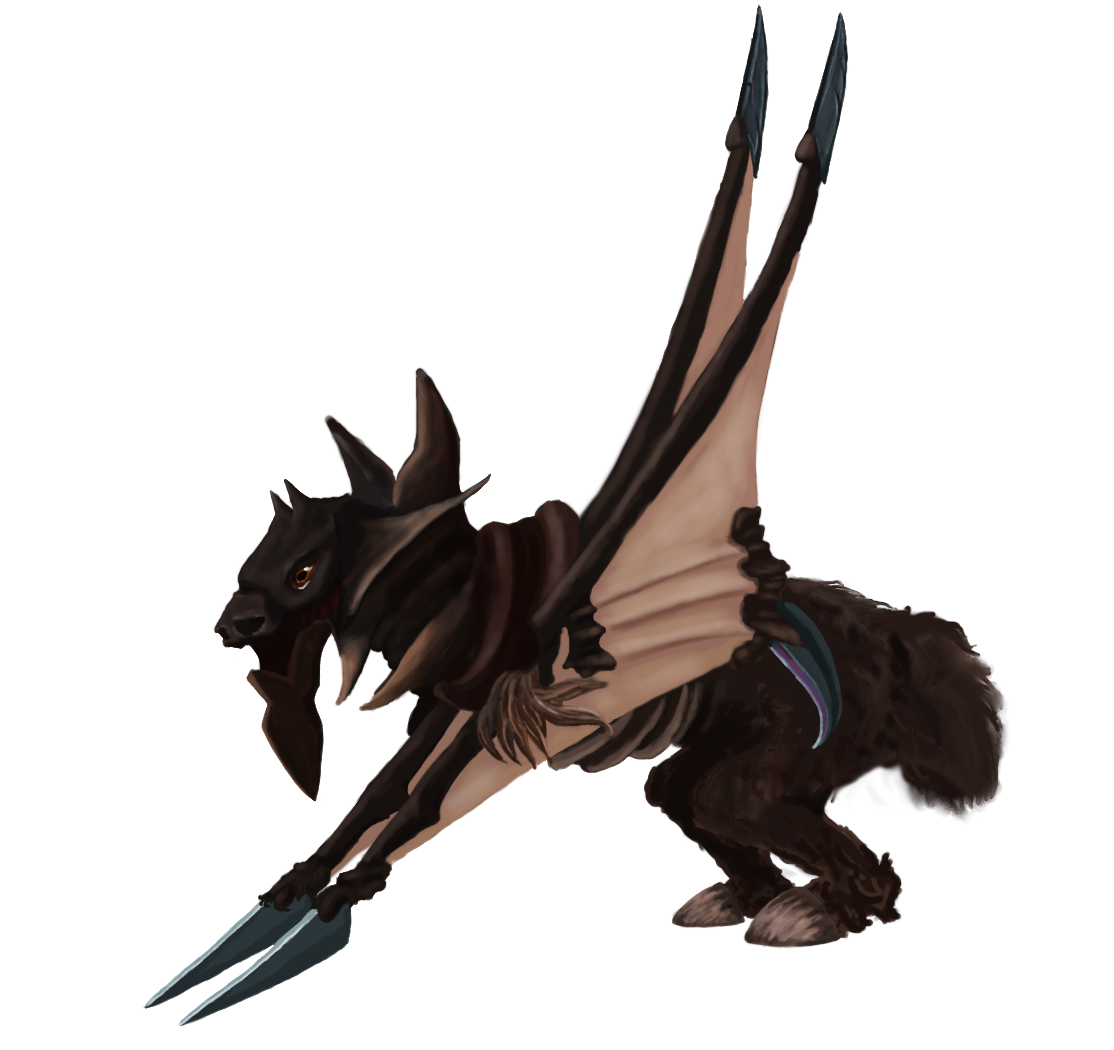
\includegraphics[width=8cm]{Pictures/Wareguard.png}
		        %\caption{Wareguard}
             \label{fig:Wareguard}
        \end{figure}
        
\section*{Artenmerkmale}

\begin{tcolorbox}[title=Artenwerte,colbacktitle=mydarkblue,tabulars={@{\extracolsep{\fill}\hspace{5mm}}cccc@{\hspace{5mm}}},boxrule=0.5pt]
    \textbf{Wunden} & \textbf{Gift} & \textbf{Psyche} & \textbf{Bewegung} \\\hline
    45 & 9 & 14 & 5 \\ \hlineB{3}
    \multicolumn{2}{ r| }{\textbf{Rasse:}} & \multicolumn{2}{ c }{Spirit} \\
    \multicolumn{2}{ r| }{\textbf{Größe:}} & \multicolumn{2}{ c }{Groß, 1.75 - 2.1 m} \\
    \multicolumn{2}{ r| }{\textbf{Gewicht:}} & \multicolumn{2}{ c }{ 90 - 140 kg} 
\end{tcolorbox}

\subsection*{Genetik der Wareguards}
\vspace*{0.75 cm}

\begin{tcolorbox}[title= Herz Genetik, colbacktitle=red, tabulars={@{\extracolsep{\fill}\hspace{5mm}}lc@{\hspace{1mm}}}, boxrule=0.5pt]
    \textbf{Rang 1:} & Aktion \verweis{sk:ausweiden} \\
    \textbf{Rang 2:} & +2 Intelligenz \\
    \textbf{Rang 3:} & +2 auf Spirit  \\
    \textbf{Rang 4:} & +2 auf Gewandtheit  \\
    \textbf{Rang 5:} & +2 Auf Geschicklichkeit \\
\end{tcolorbox}
\vspace*{0.4 cm}

\begin{tcolorbox}[title= Pik Genetik,colbacktitle=gray, tabulars={@{\extracolsep{\fill}\hspace{5mm}}lc@{\hspace{1mm}}}, boxrule=0.5pt]
    \textbf{Rang 1:} & +2 Emotionem \\
    \textbf{Rang 2:} & +6 auf Wundenmaximum \\
    \textbf{Rang 3:} & +3 auf Robustheit \\
    \textbf{Rang 4:} & Passive \verweis{sk:entziehen} \\
    \textbf{Rang 5:} & +3 auf Kraft \\
\end{tcolorbox}
\vspace*{0.4 cm}

\begin{tcolorbox}[title= Karo Genetik, colbacktitle=red, tabulars={@{\extracolsep{\fill}\hspace{5mm}}lc@{\hspace{1mm}}}, boxrule=0.5pt]
    \textbf{Rang 1:} & +1 in einem Element  \\
    \textbf{Rang 2:} & +2 auf Kreativität \\
    \textbf{Rang 3:} & +3 auf Spirit \\
    \textbf{Rang 4:} & +2 Initiative\\
    \textbf{Rang 5:} & +5 Psychemaximum \\

\end{tcolorbox}
\vspace*{0.4 cm}

\begin{tcolorbox}[title= Kreuz Genetik, colbacktitle=gray, tabulars={@{\extracolsep{\fill}\hspace{5mm}}lc@{\hspace{1mm}}}, boxrule=0.5pt]
    \textbf{Rang 1:} & +2 Spirit \\
    \textbf{Rang 2:} & Aktion \verweis{sk:aufsteigen} \\
    \textbf{Rang 3:} & +2 auf Charisma \\
    \textbf{Rang 4:} & +3 auf Willenskraft \\
    \textbf{Rang 5:} & +5 auf Giftmaximum \\
\end{tcolorbox}

\subsection*{Grundzüge}
Wareguard sind in der Lage zu jederzeit in die Lüfte aufzusteigen und zu Fliegen können jedoch durch die Abwesenheit von Greifwerkzeugen keine Waffen benutzen.\\
Dein Charakter verfügt von beginn an über die Aktionen: \verweis{sk:lebenswache} und \verweis{sk:sprungangriff}.

\subsection*{Lebenswache} \label{sk:lebenswache}
 Es ist eines Wareguards Aufgabe ihre Meister zu schützen. Hierzu sind sie bereit Dinge zu tun, die schlimmer als der Tod sind.\\
\textbf{Grundwert:} Willenskraft \\
\textbf{Anforderung:} $\Pik{}$ 10+ \\
\textbf{Reichweite:} 3 m \\
\textbf{Effekt:} Wähle eine Kreatur. Wunden die diese Kreatur erleiden würde  werden stattdessen dir zugefügt, bis zur deiner nächsten Aktionsphase.\\
\textbf{Steigerung [10]:} Effekt gilt bis zum ende der Kampfrunde, kann vorher abgebrochen werden (nur zu beginn deiner Aktionsphase).\\
\textbf{Steigerung [20]:} Du kannst 2 Kreaturen wählen.

\subsection*{Sprungangriff} \label{sk:sprungangriff}
 Es ist eines Wareguards Aufgabe ihre Meister zu schützen. Hierzu sind sie bereit Dinge zu tun, die schlimmer als der Tod sind.\\
\textbf{Grundwert:} Geschicklichkeit \\
\textbf{Kenntnisschwelle:} 2 \\
\textbf{Anforderung:} Bewegend $\Herz{}$ 15+ \\
\textbf{Reichweite:} 4 m \\
\textbf{Effekt:} \textit{Passiv.} Du springst aus mindestens 2 Metern bis zu 4 Metern auf dein Ziel und bindest es.

\begin{table}[h!]
    \centering
    \begin{tabular}{|>{\columncolor[RGB]{247, 216, 212}}l|}
    \btrule{1pt}
    \arrayrulecolor{black}
    \\
    \textbf{\large Wareguard}\\
    \\
        \begin{tabular}{c|c|c}
           \rowcolor{myred} \begin{tabular}{c}
               \rowcolor{myred}\textbf{Gefahren-}  \\
                \rowcolor{myred} \textbf{wert}\\ 
            \end{tabular} & \textbf{Fähingkeiten} & \textbf{Ausprägung}\\
            \hline
            \rowcolor{myred} 1. & -- & Wächter \\
            \rowcolor{mydarkblue} 2. & 1x Simpel &  Wächter \\
            \rowcolor{myred} 3. & 1x Erweiter & Wächter\\
            \rowcolor{mydarkblue} 4. & 1x Komplex &  Körperentw. \\
            \rowcolor{myred} 5. & (Spezifisch) &  Wächter\\
            \rowcolor{mydarkblue} 6. & -- & Charakterentw.. \\
            \rowcolor{myred} 7. & 2x Simpel &  Wächter \\
            \rowcolor{mydarkblue} 8. & 1x Erweitert & (Spezifisch)\\
            \rowcolor{myred} 9. & 1x Komplex & Wächter\\
            \rowcolor{mydarkblue} 10. & (Spezifisch) & (Spezifisch) \\
            \rowcolor{myred} 11. & -- & Körperentw.\\
            \rowcolor{mydarkblue} 12. & 1x Simpel & Wächter\\
            \rowcolor{myred} 13. & 2x Erweitert & Charakterentw..\\
            \rowcolor{mydarkblue} 14. & 1x Komplex & (Spezifisch)\\
            \rowcolor{myred} 15. & (Spezifisch) & Wächter\\
            \rowcolor{mydarkblue} 16. & -- & Körperentw.\\
            \rowcolor{myred} 17. & 1x Simpel & Charakterentw..\\
            \rowcolor{mydarkblue} 18. & 1x Erweitert & Brut \\
            \rowcolor{myred} 19. & 2x Komplex & (Spezifisch)\\
            \rowcolor{mydarkblue} 20. & (Spezifisch) & Körperentw.\\
            \rowcolor{myred} 21. & -- & Charakterentw..\\
            \rowcolor{mydarkblue} 22. & 2x Simpel & Wächter\\
            \rowcolor{myred} 23. & 2x Erweitert & Körperentw.\\
            \rowcolor{mydarkblue} 24. & 2x Komplex & Charakterentw..\\
            \rowcolor{myred} 25. & (Spezifisch) & (Spezifisch) \\
            %\rowcolor{myblue} 26. & -- & Pfad\\
            %\rowcolor{myred} 27. & 2x Simpel & \\
            %\rowcolor{myblue} 28. & 2x Erweitert& \\
            %\rowcolor{myred} 29. & 2x Komplex & \\
            %\rowcolor{myblue} 30. &  (Spezifisch) & Pfad\\
        \end{tabular}\\
        \rowcolor{myred}\\
        \btrule{1pt}
    \end{tabular}
\end{table}

\section*{Reise der Wächter}
Die wahre Bestimmung der Wareguards ist zu wachen, über was sie jetzt genau und wie sie darüber wachen ist nicht ganz klar. Sie lassen sich jedoch in vier große Kategorien unterteilen.

\subsection*{Wächter der Zeit}
Wächter der Zeit wachen über die Vergangenheit, Gegenwart und Zukunft um die Welt im zeitlichen Gleichgewicht zu halten. Dazu lernen sie die Zeit zu verstehen und zu manipulieren.
\textbf{Boni:}  +3 oder -3 auf Initiative\\
\textbf{Anfangsausrüstung:} \\
\textbf{Startfähigkeit:} \verweis{sk:beschleunigen} \\

\subsubsection*{Beschleunigen} \label{sk:beschleunigen}
Es gibt kaum ein bekanntes Wesen dass es mit dem Wissen eines Zeit Wächters über die Zeit aufnehmen kann. Das bringt dem gewieften Jäger im Kampf einige Vorteile.\\
\textbf{Effekt:} Ziehe während des Schrittes Kartenziehen eine Karte mehr. Dann lege eine Karte ab.\\
\textbf{Steigerung [15]:} Ziehe während des Schrittes Kartenziehen zwei Karte mehr. Dann lege zwei Karte ab.\\
\textbf{Steigerung [25]:} Ziehe während des Schrittes Kartenziehen drei Karte mehr. Dann lege zwei Karte ab.


\subsection*{Wächter der Welten}
Um die Unterwelt, Überwelt und heimliche Welt zu trennen, stehen die Wächter der Welten im ewigen konfilkt mit Kreaturen der Unter- und Überwelt die sich auf der heimlichen Welt niedergelassen haben.
\textbf{Boni:}  +5 auf Angriffe gegen Kreaturen der Unter- oder Überwelt.\\
\textbf{Anfangsausrüstung:} \\
\textbf{Startfähigkeit:} \verweis{sk:panzer_des_waechters} \\

\subsubsection*{Panzer des Wächters} \label{sk:panzer_des_waechters}
Die teils knochenartige, teils Fell bedeckte Oberfläche des großen Wareguardkörpers ist extrem widerstandsfest.\\
\textbf{Effekt:} Du erhältst +1 Rüstung zu Beginn des Kampfes für jeden Verbündeten in diesem Kampf.\\
\textbf{Steigerung [10]:} Du hast durch schwere Verletzungen keine Mali. Allerdings ist die fünfte schwere Verletzungen weiterhin tödlich.


\subsection*{Wächter des Spirit}
Das Spiritfeld ist älter als die Wareguards. Einie Wareguards die sehr in den Genuss des Spirits gekommen sind haben es sich zu Aufgabe gemacht diese zu schützen und zu wahren, so dass auch andere Arten in den Genuss des Spirits kommen können.
\textbf{Boni:}  +2 auf Spirit\\
\textbf{Anfangsausrüstung:} \\
\textbf{Startfähigkeit:} \verweis{sk:elementaffin} \\

\subsubsection*{Elementaffin} \label{sk:elementaffin}
Elemente sind Manifeste des Spirit, Wareguards vermögen sich auf eins zu spezialisieren. \\
\textbf{Effekt:} Wähle ein Element deiner Wahl du erhältst +3 auf jenes Element und du bist resistent gegenüber Spiritaktionen des Elements.\\
\textbf{Steigerung [10]:} +1 auf das gewählte Element.\\
\textbf{Steigerung [20]:} +2 auf das gewählte Element.\\
\textbf{Steigerung [25]:} Du bist immun gegenüber dem gewählten Element.\\


\subsection*{Wächter des Leben}
Für diese Wareguards ist das Leben von ganz großer Bedeutung. Leben ist ihnen zwar heilig, sie schützten, aber nur jenes, welches sie für Würdig halten.
\textbf{Boni:} \\
\textbf{Anfangsausrüstung:} \\
\textbf{Startfähigkeit:} \verweis{sk:heilendes_feuer} \\

\subsubsection*{Heilendes Feuer} \label{sk:heilendes_feuer}
Der Wareguard ist in der Lage die Wogen des Spirits umzufädeln und Diener der goldenen Flamme in eine Aura der heilenden Symphonie zu binden. \\
\textbf{Effekt:} Wähle zu Beginn der Kampfrunde eine Kreatur, jene wird von dem Effekt Brennend geheilt anstatt das sie Verletzungen erleidet.\\
\textbf{Steigerung [15]:} Du kannst eine weiter Kreatur wählen die den Effekt erhält.\\
\textbf{Steigerung [25]:} Alle befreundete Kreaturen erhalten den Effekt.\\